\documentclass[11pt]{article}

\usepackage{amsmath}
\usepackage{mathtools}
\usepackage{amssymb}
\usepackage{wrapfig}
\usepackage{fancyhdr}
\usepackage{tikz-qtree}
\usepackage{tikz-qtree-compat}
\usepackage[normalem]{ulem}
\usepackage{tikz}
\usepackage{graphicx}
\usepackage{lineno}
\usepackage{floatrow}
\usepackage{bm}

\DeclareMathOperator*{\argmin}{argmin}
\DeclareMathOperator*{\argmax}{argmax}

\oddsidemargin0cm
\topmargin-2cm
\textwidth16.5cm
\textheight23.5cm 

\newcommand{\question}[2] {\vspace{.25in} \hrule\vspace{0.5em}
\noindent{\bf #1: #2} \vspace{0.5em}
\hrule \vspace{.10in}}
\renewcommand{\part}[1] {\vspace{.10in} {\bf (#1)}}
\linespread{1.5}

\setlength{\parindent}{0pt}
\setlength{\parskip}{5pt plus 1pt}
 
\DeclarePairedDelimiter\abs{\lvert}{\rvert}%


\begin{document}
\medskip        

\thispagestyle{plain}
{\Large Interrogating theoretical models of neural computation with deep inference} \\
Sean R. Bittner$^{1}$, Agostina Palmigiano$^{1}$, Alex T. Piet$^{2,3,4}$, Chunyu A. Duan$^{5}$, Carlos D. Brody$^{2,3,6}$, \\
Kenneth D. Miller$^{1}$, and John P. Cunningham$^{7}$.

{\small
$^{1}$Department of Neuroscience, Columbia University, \\
$^{2}$Princeton Neuroscience Institute, \\
$^{3}$Princeton University, \\
$^{4}$Allen Institute for Brain Science, \\
$^{5}$Institute of Neuroscience, Chinese Academy of Sciences, \\
$^{6}$Howard Hughes Medical Institute, \\
$^{7}$Department of Statistics, Columbia University
}

\linenumbers
\section{Abstract}
A cornerstone of theoretical neuroscience is the circuit model: a system of equations that captures a hypothesized neural mechanism.  
Such models are valuable when they give rise to an experimentally observed phenomenon -- whether behavioral or in terms of neural activity -- and thus can offer insights into neural computation.
The operation of these circuits, like all models, critically depends on the choices of model parameters.
When analytic derivation of the relationship between model parameters and computational properties is intractable, approximate inference and simulation-based techniques are relied upon for scientific insight.
%Historically, the gold standard has been to analytically derive the relationship between model parameters and computational properties.  
%However, this enterprise quickly becomes infeasible as biologically realistic constraints are included into the model increasing its complexity, often resulting in \emph{ad hoc} approaches to understanding the relationship between model and computation.
We bring the use of deep generative models for probabilistic inference to bear on this problem, learning complex distributions of parameters that produce the specified properties of computation.
Our novel method solves the inverse problem by identifying the full space of parameters producing the emergent property.
%Importantly, the techniques we introduce offer a principled means to understand the implications of model parameter choices on computational properties of interest.  
We motivate this methodology with a worked example analyzing sensitivity in the stomatogastric ganglion.  
%We then use it to go beyond linear theory of neuron-type input-responsivity in a model of primary visual cortex, gain a mechanistic understanding of rapid task switching in superior colliculus models, and attribute error to connectivity properties in recurrent neural networks solving a simple mathematical task.
We then use it to reveal the key factors of variability in a model of primary visual cortex, gain a mechanistic understanding of rapid task switching in superior colliculus models, and scale inference of large low-rank RNN's exhibiting stable amplification.
This work illustrates how we can further leverage the power of deep learning towards solving inverse problems in theoretical neuroscience.
%More generally, this work suggests a departure from realism vs tractability considerations, towards the use of modern machine learning for sophisticated interrogation of biologically relevant models.

\section{Introduction}
The fundamental practice of theoretical neuroscience is to use a mathematical model to understand neural computation, whether that computation enables perception, action, or some intermediate processing.  
A neural computation is systematized with a set of equations -- the model -- and these equations are motivated by biophysics, neurophysiology, and other conceptual considerations \cite{kopell1988coupled,  marder1998biophysics, abbott2008theoretical, wang2010neurophysiological}.
The function of this system is governed by the choice of model \emph{parameters}, which when configured in a particular way, give rise to a measurable signature of a computation.   
The work of analyzing a model then requires solving the inverse problem: given a computation of interest, how can we reason about particular parameter configurations?  
%The inverse problem is crucial for reasoning about likely parameter values, uniquenesses and degeneracies, attractor states and phase transitions, and predictions made by the model.
The inverse problem is crucial for reasoning about likely parameter values, uniquenesses and degeneracies, and predictions made by the model \cite{gutenkunst2007universally, o2014cell}.

Consider the idealized practice: one carefully designs a model and analytically derives how computational properties determine model parameters.
Seminal examples of this gold standard (which often adopt approaches from statistical physics) include our field's understanding of memory capacity in associative neural networks \cite{hopfield1982neural}, chaos and autocorrelation timescales in random neural networks \cite{sompolinsky1988chaos}, the paradoxical effect \cite{tsodyks1997paradoxical}, and decision making \cite{wong2006recurrent}.
Unfortunately, as circuit models include more biological realism, theory via analytical derivation becomes intractable.
%This creates an unfavorable tradeoff.  On the one hand, one may tractably analyze systems of equations with unrealistic assumptions (for example symmetry or gaussianity), mathematically formalizing how parameters affect computation in a too-simple model.  
%On the other hand, one may choose a more biologically accurate, scientifically relevant model at the cost of \emph{ad hoc} approaches to analysis (such as simply examining simulated activity), potentially resulting in bad inference of parameters and thus erroneous scientific predictions or conclusions.
Alternatively, we can gain insight into these complex models by identifying the full distribution of parameters consistent with specified emergent phenomena.
By solving the inverse problem in this way, scientists can reason about the sensitivity and robustness of the model with respect to different parameter combinations \cite{foster1993significance, prinz2004similar, achard2006complex, o2014cell, alonso2019visualization}.

The preferred formalism for parameter identification in science is statistical inference, which has been used to great success in neuroscience through the stipulation of statistical generative models \cite{kass2001spike, brown1998statistical, paninski2004maximum, truccolo2005point, schneidman2006weak, druckmann2007novel, turner2007maximum, byron2009gaussian, macke2011empirical, park2011bayesian, granot2013stimulus, latimer2015single, lakshminarasimhan2018dynamic, duncker2019learning, ladenbauer2019inferring} (see review, \cite{paninski2018neural}). 
%Exact Bayesian inference is rarely tractable, so Markov chain Monte Carlo (MCMC) and variation inference (VI) techniques are used in practice.
However, most neural circuit models in theoretical neuroscience stipulate a noisy system of differential equations that can only be sampled or realized through forward simulation; they lack the explicit likelihood central to the probabilistic modeling toolkit.
Therefore, the most popular approaches to the inverse problem have been likelihood-free methods such as approximate Bayesian computation (ABC) \cite{sisson2007sequential, liepe2014framework}, in which reasonable parameters are obtained via simulation and rejection.

% now transition to deep ML...
%Of course, this same tradeoff has been confronted in many scientific fields characterized by the need to do inference in complex models.
%In response, the machine learning community has made remarkable progress in recent years, via the use of deep neural networks as a powerful inference engine: a flexible function family that can map observed phenomena (in this case the measurable signal of some computation) back to probability distributions quantifying the likely parameter configurations.  
Of course, the challenge of doing inference in complex models has arisen in many scientific fields.
In response, the machine learning community has made remarkable progress in recent years, via the use of deep neural networks as powerful inference engines: a flexible function family that can map observations back to probability distributions quantifying the likely parameter configurations. 
%One celebrated example of this approach from machine learning, of which we draw key inspiration for this work, is the variational autoencoder \cite{kingma2013auto, rezende2014stochastic}, which uses a deep neural network to induce an (approximate) posterior distribution on hidden variables in a latent variable model, given data. 
One celebrated example of this approach from machine learning, of which we draw key inspiration for this work, is the variational autoencoder (VAE) \cite{kingma2013auto, rezende2014stochastic}, which uses a deep neural network to induce an (approximate) posterior distribution on hidden variables in a latent variable model, given data. 
Indeed, these tools have been used to great success in neuroscience as well, in particular for interrogating hidden states in models of both cortical population activity \cite{gao2016linear, zhao2017recursive, barello2018sparse, pandarinath2018inferring} and animal behavior \cite{wiltschko2015mapping, johnson2016composing, batty2019behavenet}. 
These works have used deep neural networks to expand the domain of neural data sets amenable to statistical modeling \cite{paninski2018neural}.

% What's wrong with existing methodology:
Existing approaches to the inverse problem in theoretical neuroscience fall short in three key ways. 
First, theoretical models of neural computation aim to reflect a complex biological reality, and as a result, such models lack tractable likelihoods.
Without an efficient calculation of the probability of model properties given model parameters, neuroscientists resort to approximate Bayesian computation \cite{beaumont2002approximate, marjoram2003markov, sisson2007sequential}, which requires a rejection heuristic, scales poorly, and only produces sets of accepted parameters lacking probabilities.
Second, there is an undesirable trade-off between the flexibility and sampling speed of approximated posterior distributions.
Sampling-based inference approaches (e.g. ABC and Markov chain Monte Carlo (MCMC) \cite{hastings1970monte, metropolis1953equation}) confer flexible approximations, yet scale poorly in number of parameters.
While variational inference (VI) \cite{saul1998mean} often results in fast posterior sampling, existing practice relies heavily on simplified classes of distributions \cite{rezende2015variational}.  
Third, such parameter inference methods are designed to operate on experimentally collected data-sets.
Ultimately, the objects of interest in theoretical neuroscience are phenomena or features of the model rather than singular data-sets.

%However, these inference tools have not significantly influenced the study of theoretical neuroscience models, for at least three reasons.
%First, at a practical level, the nonlinearities and dynamics of many theoretical models are such that conventional inference tools typically produce a narrow set of insights into these models.
%Indeed, only in the last few years has deep learning research advanced to a point of relevance to this class of problem.
%Second, the object of interest from a theoretical model is not typically data itself, but rather a qualitative phenomenon -- inspection of model behavior, or better, a measurable signature of some computation -- an \emph{emergent property} of the model.  
%Third, because theoreticians work carefully to construct a model that has biological relevance, such a model as a result often does not fit cleanly into the framing of a statistical model.
%Technically, because many such models stipulate a noisy system of differential equations that can only be sampled or realized through forward simulation, they lack the explicit likelihood and priors central to the probabilistic modeling toolkit.

% now we've constructed the tension that theory models need this and statistical models know how to do this... now connect!
To address these three challenges, we developed an inference methodology -- `emergent property inference' -- which learns a distribution over parameter configurations in a theoretical model.  
This distribution has two critical properties: \emph{(i)} it is chosen such that draws from the distribution (parameter configurations) correspond to systems of equations that give rise to a specified emergent property (a set of constraints); and \emph{(ii)} it is chosen to have maximum entropy given those constraints, such that we identify all likely parameters and can use the distribution to reason about parametric sensitivity and degeneracies \cite{transtrum2015perspective}.  
%First, we stipulate a bijective deep neural network that induces a flexible family of probability distributions over model parameterizations with a probability density we can calculate \cite{rezende2015variational, dinh2016density, papamakarios2017masked}.
%Second, we quantify the notion of emergent properties as a set of moment constraints on datasets generated by the model.  
%Thus, an emergent property is not a single data realization, but a phenomenon or a feature of the model, which is ultimately the object of interest in theoretical neuroscience.
%Conditioning on an emergent property requires a variant of deep probabilistic inference methods, which we have previously introduced \cite{loaiza2017maximum}.
%Third,  because we cannot assume the theoretical model has explicit likelihood on data or the emergent property of interest, we use stochastic gradient techniques in the spirit of likelihood free variational inference \cite{tran2017hierarchical}.    
%Taken together, emergent property inference (EPI) provides a methodology for inferring parameter configurations consistent with a particular emergent phenomena in theoretical models.
%We use a classic example of parametric degeneracy in a biological system, the stomatogastric ganglion \cite{goldman2001global}, to motivate and clarify the technical details of EPI.
First, we use stochastic gradient techniques in the spirit of likelihood-free variational inference \cite{tran2017hierarchical} to enable inference in likelihood-free models of neural computation.
Second, we stipulate a bijective deep neural network that induces a flexible family of probability distributions over model parameterizations with a probability density we can calculate \cite{rezende2015variational, dinh2017density, papamakarios2017masked}, which confers fast sampling and sensitivity measurements.
Third, we quantify the notion of emergent properties as a set of moment constraints on datasets generated by the model.  
Thus, an emergent property is not a single data realization, but a phenomenon or a feature of the model.
Conditioning on an emergent property requires a variant of deep probabilistic inference methods, which we have previously introduced \cite{loaiza2017maximum}.
Taken together, emergent property inference (EPI) provides a methodology for inferring parameter configurations consistent with a particular emergent phenomena in theoretical models.
We use a classic example of parametric degeneracy in a biological system, the stomatogastric ganglion \cite{goldman2001global}, to motivate and clarify the technical details of EPI.

Equipped with this methodology, we then investigated three models of current importance in theoretical neuroscience.
These models were chosen to demonstrate generality through ranges of biological realism (from conductance-based biophysics to recurrent neural networks), neural system function (from pattern generation to decision making), and network scale (from four to hundreds of neurons).
%First, we use EPI to produce a set of verifiable hypotheses of input-responsivity in a four neuron-type dynamical model of primary visual cortex; we then validate these hypotheses in the model.
First, we use EPI to understand the characteristics of noise across mulitple neuron-type populations that govern variability in a model of primary visual cortex.
%Second, we demonstrated how the systematic application of EPI to levels of task performance can generate experimentally testable hypotheses regarding connectivity in superior colliculus.  
Then, we use EPI to infer multiple regimes of superior colliculus connectivity that perform rapid task switching.
The novel scientific insights offered by EPI contextualize and clarify the previous studies exploring these models \cite{litwin2016inhibitory, duan2018collicular}.
%Third, we use EPI to uncover the sources of error in a low-rank recurrent neural network executing a simple mathematical task.  
Finally, we emphasize the scalability of EPI by inferring high-dimensional distributions of RNNs exhibiting stable amplification.
These results point to the value of deep inference for the interrogation of biologically relevant models.

%-------------------

%%%%%%%%%%%%%%%%%%%%%%%%%%%%%%%%%%%
%%%%%%%%%%%%%%%%%%%%%%%%%%%%%%%%%%%

\section{Results}
\subsection{Motivating emergent property inference of theoretical models} \label{results_motivating}

%Consideration of the typical workflow of theoretical modeling clarifies the need for emergent property inference.  
Consideration of the typical workflow of theoretical modeling clarifies the need for emergent property inference.  
First, one designs or chooses an existing model that, it is hypothesized, captures the computation of interest. 
To ground this process in a well-known example, consider the stomatogastric ganglion (STG) of crustaceans, a small neural circuit which generates multiple rhythmic muscle activation patterns for digestion \cite{marder2002cellular}.
Despite full knowledge of STG connectivity and a precise characterization of its rhythmic pattern generation, biophysical models of the STG have complicated relationships between circuit parameters and neural activity \cite{goldman2001global, prinz2004similar}.
%A model of the STG \cite{gutierrez2013multiple} is shown schematically in Figure \ref{fig:STG}A, and note that the behavior of this model will be critically dependent on its parameterization -- the choices of conductance parameters $z = [g_{\text{el}}, g_{\text{synA}}]$.
A subcircuit model of the STG \cite{gutierrez2013multiple} is shown schematically in Figure \ref{fig:STG}A, and note that the behavior of this model will be critically dependent on its parameterization -- the choices of conductance parameters $\mathbf{z} = [g_{\text{el}}, g_{\text{synA}}]$.
Specifically, the two fast neurons ($f1$ and $f2$) mutually inhibit one another, and oscillate at a faster frequency than the mutually inhibiting slow neurons ($s1$ and $s2$).  
The hub neuron (hub) couples with either the fast or slow population or both.  

%Second, once the model is selected, one defines the emergent property, the measurable signal of scientific interest.  
Second, once the model is selected, one defines the emergent phenomena of scientific interest.
%To continue our running STG example, one such emergent property is the phenomenon of \emph{network syncing} -- in certain parameter regimes, the frequency of the hub neuron matches that of the fast and slow populations at an intermediate frequency.
In the STG example, we are concerned with neural spiking frequency, which emerges from the dynamics of the circuit model \ref{fig:STG}B.
%One such emergent property is the phenomenon of \emph{unified intermediacy} -- in certain parameter regimes, the frequency of all neurons match at an intermediate firing rate.
An interesting emergent property of this stochastic model is when the hub neuron fires at an intermediate frequency between the intrinsic spiking rates of the fast and slow populations.
%This emergent property is shown in Figure \ref{fig:STG}D at a frequency of 0.53Hz.
This emergent property is shown in Figure \ref{fig:STG}C at an average frequency of 0.55Hz.

%Third, qualitative parameter analysis ensues: since precise mathematical analysis is intractable in this model, a brute force sweep of parameters is done \cite{gutierrez2013multiple}.
%Subsequently, a qualitative description is formulated to describe the different parameter configurations that lead to the emergent property.  
%In this last step lies the opportunity for a precise quantification of the emergent property as a statistical feature of the model. 
% Once we have such a methodology, we can infer a probability distribution over parameter configurations that produce this emergent property.
Third, parameter analyses ensue: brute-force parameter sweeps, ABC sampling, and sensitivity analyses are all routinely used to reason about what parameter configurations lead to an emergent property.
In this last step lies the opportunity for a precise quantification of the emergent property as a statistical feature of the model.
Once we have such a methodology, we can infer a probability distribution over parameter configurations that produce this emergent property.

%A. For a choice of model (STG) and emergent property (network syncing), emergent property inference (EPI, gray box) learns a distribution of the model parameters $z = \left[g_{\text{el}}, g_{\text{synA}} \right]$ producing network syncing.  
%In the STG model, jagged connections indicate electrical coupling having electrical conductance $g_{\text{el}}$. 
%Other connections in the diagram are inhibitory synaptic projections having strength $g_{\text{synA}}$ onto the hub neuron, and $g_{\text{synB}}=5$nS for mutual inhibitory connections.  
%Network syncing traces are colored by log probability density of their generating parameters (stars) in the EPI-inferred distribution.  
%B. The EPI distribution of STG model parameters producing network syncing.  
%Samples are colored by log probability density.  
%Distribution contours of emergent property value error are shown at levels of $2.5 \times 10^{-5}$, $5 \times 10^{-5}$, $1 \times 10^{-4}$, $2 \times 10^{-4}$, and $4 \times 10^{-4}$ (dark to light gray).  
%Eigenvectors of the Hessian at the mode of the inferred distribution are indicated as $\mathbf{v}_1$ (solid) and $\mathbf{v}_2$ (dashed) with lengths scaled by the square root of the absolute value of their eigenvalues.  
%Simulated activity is shown for three samples (stars). 
%(Inset) Sensitivity of the system with respect to network syncing along all dimensions of parameter space away from the mode.  
%$v_1$ is sensitive to network syncing ($p<10^{-4}$), while $v_2$ is not ($p=0.67$) (see Section \ref{methods_STG}).  
%C. Deep probability distributions map a latent random variable $\mathbf{w}$ through a deep neural network with weights and biases $\bm{\theta}$ to parameters $\mathbf{z} = f_{\bm{\theta}}(\mathbf{w})$ distributed as $q_{\bm{\theta}}(\mathbf{z})$. 
%D. EPI optimization: To learn the EPI distribution $q_{\bm{\theta}}(\mathbf{z})$ of model parameters that produce an emergent property, the emergent property statistics $T(\mathbf{x})$ are set in expectation over model parameter samples $\mathbf{z} \sim q_{\bm{\theta}}(\mathbf{z})$ and model simulations $\mathbf{x} \sim p(\mathbf{x} \mid \mathbf{z})$ to emergent property values $\bm{\mu}$.
\begin{figure}
\begin{center}
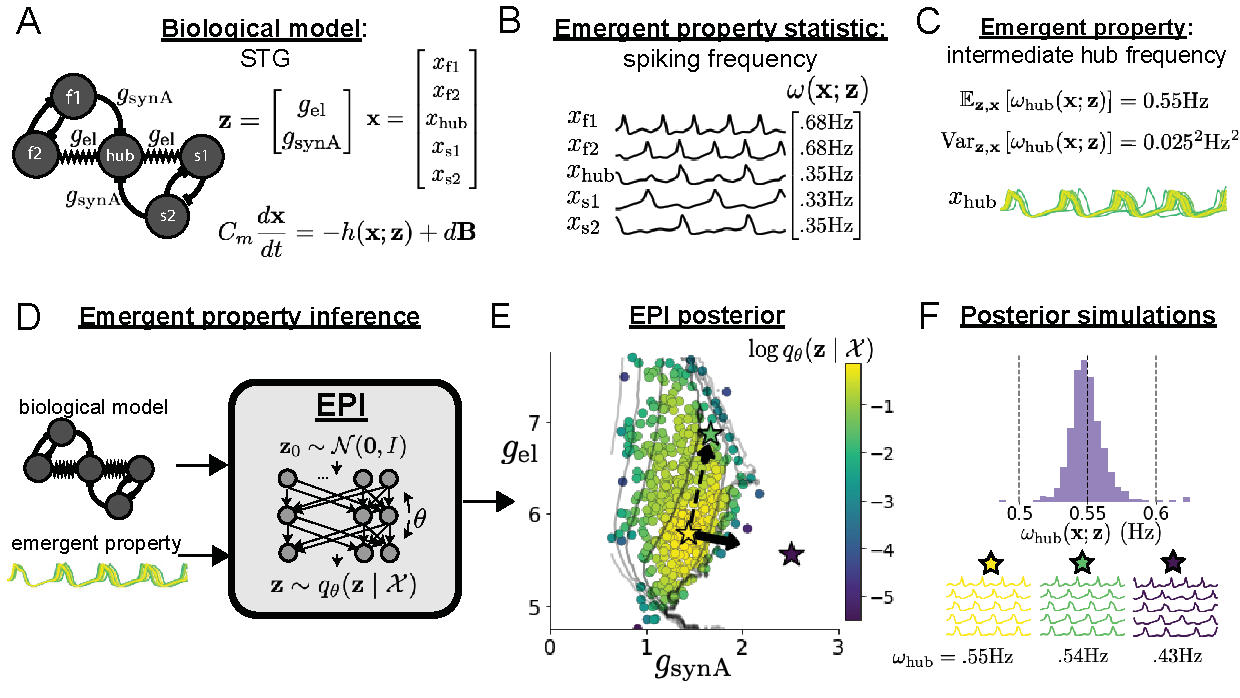
\includegraphics[scale=0.8]{figures/fig1/fig1.pdf}
\end{center}
\caption{\small Emergent property inference (EPI) in the stomatogastric ganglion.  
\textbf{A}. Conductance-based biophysical model of the STG subcircuit.
In the STG model, jagged connections indicate electrical coupling having electrical conductance $g_{\text{el}}$. 
Other connections in the diagram are inhibitory synaptic projections having strength $g_{\text{synA}}$ onto the hub neuron, and $g_{\text{synB}}=5$nS for mutual inhibitory connections.  
Parameters are represented by the vector $\mathbf{z}$ and membrane potentials by the vector $\mathbf{x}$.
The evolution of this model's activity $\mathbf{x}(t)$ is predicated by differential equations.
\textbf{B}. Spiking frequency $\omega(\mathbf{x}; \mathbf{z})$ is an emergent property statistic. 
In this example, spiking frequency is measured from simulated activity of the STG model at parameter choices of $g_{\text{el}} = 4.5$nS and $g_{\text{synA}} = 3$nS.
\textbf{C}. The emergent property of intermediate hub frequency, in which the hub neuron fires at a rate between the fast and slow frequencies.
This emergent property is defined by a mean and variance on the emergent property statistic.
Simulated activity traces are colored by log probability density of their generating parameters in the EPI-inferred distribution (Panel E).
\textbf{D}. For a choice of model and emergent property, emergent property inference (EPI) learns a deep probability distribution of parameters $\mathbf{z}$.
Deep probability distributions map a simple random variable $\mathbf{z}_0$ through a deep neural network with weights and biases $\bm{\theta}$ to parameters $\mathbf{z} = g_{\bm{\theta}}(\mathbf{z}_0)$.
In EPI optimization, stochastic gradient steps in $\bm{\theta}$ are taken such that entropy is maximized, and the emergent property $\mathcal{X}$ is produced.
The EPI posterior distribution is denoted $q_{\bm{\theta}}(\mathbf{z} \mid \mathcal{X})$. 
\textbf{E}. The EPI posterior producing intermediate hub frequency.
Samples are colored by log probability density.  
Distribution contours of average hub neuron frequency from mean of .55 Hz are shown at levels of $.525$, $.53$, ... $.575$ Hz (dark to light gray away from mean).
Eigenvectors of the Hessian at the mode of the inferred distribution are indicated as $\mathbf{v}_1$ (solid) and $\mathbf{v}_2$ (dashed) with lengths scaled by the square root of the absolute value of their eigenvalues.  
%(Inset) Sensitivity of the system with respect to network syncing along all dimensions of parameter space away from the mode.  
\textbf{F} Simulations from parameters in E.  
(Top) The predictive distribution of the posterior obeys the emergent property.
The black and gray dashed lines show the mean and two standard deviations according the emergent property, respectively.
(Bottom) Simulations at the starred parameter values.
 }
 \label{fig:STG}
\end{figure}


%Before presenting technical details (in the following section), let us understand emergent property inference schematically:  EPI (Fig. \ref{fig:STG}A gray box) takes, as input, the model and the specified emergent property, and as its output, produces the parameter distribution shown in Figure \ref{fig:STG}B.
Before presenting technical details (in the following section), let us understand emergent property inference schematically:  EPI (Fig. \ref{fig:STG}D) takes, as input, the model and the specified emergent property, and as its output, produces the parameter distribution  EPI (Fig. \ref{fig:STG}E).  
This distribution -- represented for clarity as samples from the distribution -- is then a scientifically meaningful and mathematically tractable object.  
In the STG model, this distribution can be specifically queried to reveal the prototypical parameter configuration for network syncing (the mode; Figure \ref{fig:STG}E yellow star), and how network syncing decays based on changes away from the mode.
The eigenvectors (of the Hessian of the distribution at the mode) quantitatively formalize the robustness of intermediate hub frequency (Fig. \ref{fig:STG}E solid ($v_1$) and dashed  ($v_2$) black arrows).
Indeed, samples equidistant from the mode along these EPI-identified dimensions of sensitivity ($v_1$) and degeneracy ($v_2$) agree with error contours (Fig. \ref{fig:STG}E contours) and have diminished or preserved hub frequency, respectively (Fig. \ref{fig:STG}F activity traces) (see Section \ref{methods_STG}).

\subsection{A deep generative modeling approach to emergent property inference} \label{results_dgm}
Emergent property inference (EPI) systematizes the three-step procedure of the previous section.
%First, we consider the model as a coupled set of differential (and potentially stochastic) equations \cite{gutierrez2013multiple}.  
First, we consider the model as a coupled set of differential equations \cite{gutierrez2013multiple}.  
In the running STG example, the model activity $\mathbf{x} = \left[ x_{\text{f1}}, x_{\text{f2}}, x_{\text{hub}}, x_{\text{s1}}, x_{\text{s2}} \right]$ is the membrane potential for each neuron, which evolves according to the biophysical conductance-based equation:
\begin{equation} 
\begin{split}
C_m \frac{d\mathbf{x}(t)}{dt} = -h(\mathbf{x}(t); \mathbf{z}) + d\mathbf{B}
 \end{split}
\end{equation} 
where $C_m$=1nF, and $\mathbf{h}$ is a sum of the leak, calcium, potassium, hyperpolarization, electrical, and synaptic currents, all of which have their own complicated dependence on $\mathbf{x}$ and $\mathbf{z} = [g_{\text{el}}, g_{\text{synA}}]$, and $d\mathbf{B}$ is white gaussian noise (see Section \ref{methods_STG}).

%Second, we define the emergent property, which as above is network syncing: oscillation of the entire population at an intermediate frequency of our choosing (Figure \ref{fig:STG}A bottom).
Second, we define the emergent property, which as above is ``intermediate hub  frequency" (Figure \ref{fig:STG}C).
%Quantifying this phenomenon is straightforward: we define network syncing to be that each neuron's spiking frequency -- denoted $\omega_{\text{f1}}(\mathbf{x})$, $\omega_{\text{f2}}(\mathbf{x})$, etc. -- is close to an intermediate frequency of 0.53Hz.  
%Mathematically, we achieve this via constraints on the mean and variance of $\omega_\alpha(\mathbf{x})$ for each neuron $\alpha \in \{ \text{f1}, \text{f2}, \text{hub}, \text{s1}, \text{s2} \}$:
Quantifying this phenomenon is straightforward: we stipulate that the hub neuron's spiking frequency -- denoted $\omega_{\text{hub}}(\mathbf{x})$ is close to an intermediate frequency of 0.55Hz.  
Mathematically, we achieve this via constraints on the mean and variance of the hub neuron spiking frequency.

%\begin{equation}\label{eq:EP}
 %\mathbb{E}\left[T(x) \right] ~~\triangleq~~ \mathbb{E}\begin{bmatrix} \omega_{\text{f1}}(x) \\ \vdots \\ (\omega_{\text{f1}}(x) - 0.53)^2 \\ \vdots \end{bmatrix} ~~=~~  
 %\begin{bmatrix} 0.53 \\ \vdots \\ 0.025^2 \\ \vdots \end{bmatrix} ~~\triangleq~~ \mu,
 %\end{equation}
\begin{equation}\label{eq:EP_STG}
\begin{split}
\mathcal{X} ~~:~~ \mathbb{E}_{\mathbf{z},\mathbf{x}}\left[f(\mathbf{x}; \mathbf{z})\right] &~~\triangleq~~  \mathbb{E}_{\mathbf{z},\mathbf{x}}\begin{bmatrix} \omega_{\text{hub}}(\mathbf{x}; \mathbf{z}) \end{bmatrix}  ~~=~~  \begin{bmatrix} 0.55 \end{bmatrix} ~~\triangleq~~ \bm{\mu}  \\ 
 \text{Var}_{\mathbf{z},\mathbf{x}}\left[f(\mathbf{x}; \mathbf{z})\right] &~~\triangleq~~ \text{Var}_{\mathbf{z},\mathbf{x}}\begin{bmatrix} \omega_{\text{hub}}(\mathbf{x}; \mathbf{z}) \end{bmatrix}  ~~=~~  \begin{bmatrix} 0.025^2 \end{bmatrix} ~~\triangleq~~ \bm{\sigma}^2 .
\end{split}
\end{equation}

%which completes the quantification of the emergent property.
The emergent property statistic $f(\mathbf{x}; \mathbf{z}) = \omega_{\text{hub}}(\mathbf{x}; \mathbf{z})$ along with its constrained mean $\bm{\mu}$ and variance $\bm{\sigma}^2$ define the emergent property denoted $\mathcal{X}$.

Third, we perform emergent property inference: we find a distribution over parameter configurations $\mathbf{z}$, and insist that samples from this distribution produce the emergent property; in other words, they obey the constraints introduced in Equation \ref{eq:EP_STG}.  
This distribution will be chosen from a family of probability distributions $\mathcal{Q} = \left\{ q_{\bm{\theta}}(\mathbf{z}) : \bm{\theta} \in \Theta \right\}$, defined by a deep generative distribution of the normalizing flow class \cite{rezende2015variational, dinh2017density, papamakarios2017masked} -- neural networks which transform a simple distribution into a suitably complicated distribution (as is needed here).  
This deep distribution is represented in Figure \ref{fig:STG}C (see Section \ref{methods_EPI}).  
Then, mathematically, we must solve the following optimization program: 
%\begin{equation} \label{eq:EPI}
%\begin{split}
%&\argmax_{q_{\bm{\theta}} \in \mathcal{Q}} H(q_{\bm{\theta}}(\mathbf{z})) \\
%&\text{  s.t.  } \mathbb{E}_{\mathbf{z} \sim q_{\bm{\theta}}}\left[ \mathbb{E}_{\mathbf{x} \sim p(\mathbf{x} \mid \mathbf{z})}\left[T(\mathbf{x})\right] \right] = \bm{\mu}, \\
%\end{split}
%\end{equation}
\begin{equation} \label{eq:EPI}
\begin{split}
q_{\bm{\theta}}(\mathbf{z} \mid \mathcal{X}) ~~=~~ &\argmax_{q_{\bm{\theta}} \in \mathcal{Q}} H(q_{\bm{\theta}}(\mathbf{z})) \\
&\text{  s.t.  } ~\mathcal{X}:~~ \mathbb{E}_{\mathbf{z},\mathbf{x}}\left[f(\mathbf{x}; \mathbf{z})\right] = \bm{\mu}, \text{Var}_{\mathbf{z},\mathbf{x}}\left[f(\mathbf{x}; \mathbf{z})\right] = \bm{\sigma}^2 \\
\end{split}
\end{equation}
%where $T(\mathbf{x}), \bm{\mu}$ are defined as in Equation \ref{eq:EP}, and $p(\mathbf{x} | \mathbf{z})$ is the intractable distribution of data from the model, $\mathbf{x}$, given that model's parameters $\mathbf{z}$ (we access samples from this distribution by running the model forward).
where $f(\mathbf{x}, \mathbf{z}), \bm{\mu}$, and $\bm{\sigma}$ are defined as in Equation \ref{eq:EP}.
According to the emergent property of interest, $f(\mathbf{x}, \mathbf{z})$ may contain multiple statistics, in which case the mean and variance vectors $\bm{\mu}$ and $\bm{\sigma}^2$ match this dimension.
%The purpose of each element in this program is detailed in Figure \ref{fig:STG}D.
Finally, we recognize that many distributions in $\mathcal{Q}$ will respect the emergent property constraints, so we select that which has maximum entropy.
This principle, captured in Equation \ref{eq:EPI} by the primal objective $H$, identifies parameter distributions with minimal assumptions beyond some chosen structure \cite{jaynes1957information, elsayed2017structure, loaiza2017maximum, savin2017maximum}.
Such a normative principle of maximum entropy, which is also that of Bayesian inference, naturally fits with our scientific objective of reasoning about parametric sensitivity and robustness. 
The recovered distribution of EPI is as variable as possible along each parametric manifold such that it produces the emergent property.

EPI optimizes the weights and biases $\bm{\theta}$ of the deep network (which induces the probability distribution) by iteratively solving Equation \ref{eq:EPI}. 
The optimization is complete when the sampled models with parameters $\mathbf{z} \sim q_{\bm{\theta}}(z \mid \mathcal{X})$ produce activity consistent with the specified emergent property (Fig. S4).
%Such convergence is evaluated with a hypothesis test that the mean of each emergent property statistic is not different than its emergent property value (see Section \ref{methods_AL_opt}). 
Such convergence is evaluated with a hypothesis test that the means and variances of each emergent property statistic are not different than their constrained values (see Section \ref{methods_AL_opt}). 
Further validation of EPI is available in the supplementary materials, where we analyze a simpler model for which ground-truth statements can be made (Section \ref{methods_2DLDS}).

In relation to broader methodology, inspection of the EPI objective reveals a natural relationship to posterior inference.
%Specifically, EPI executes variational inference in an exponential family model, the sufficient statistics and mean parameter of which are defined by the emergent property statistics and values, respectively (see Section \ref{methods_VI}).
%Specifically, EPI executes variational inference in an exponential family model, the sufficient statistics and mean parameter of which are defined by $f(\mathbf{x})$, $\bm{\mu}$ and $\bm{\sigma}$ (see Section \ref{methods_VI}).
Specifically, EPI executes a novel variant of  Bayesian inference with a uniform prior and a gaussian likelihood on the emergent property statistic (see Section \ref{methods_ME_EF}).
A key advantage of EPI over established Bayesian inference is that the predictions made by the inferred distribution are constrained to produce the specified emergent property.
%Equipped with this method, we may examine structure in such inferred distributions or make comparisons between inferred distributions at graded values of emergent property statistics.
Equipped with this method, we may examine structure in posterior distributions or make comparisons between posteriors conditioned at different levels of the same emergent property statistic.
In Sections \ref{results_V1} and \ref{results_SC}, we prove out the value of EPI by using it to investigate and produce novel insights into two prominent models in neuroscience. 
Subsequently in Section \ref{results_LRRNN}, we show EPI's superiority in parameter scalability and fidelity of the posterior predictive distribution by conditioning on stable amplification in low-rank RNNs.

%%%%%%%%%%%%%%%%%%%%%%%%%%%%
\subsection{EPI reveals how neuron-type specific noise governs variability in the stochastic stabilized supralinear network} \label{results_V1}

\begin{figure}
\vspace{-1cm}
\begin{center}
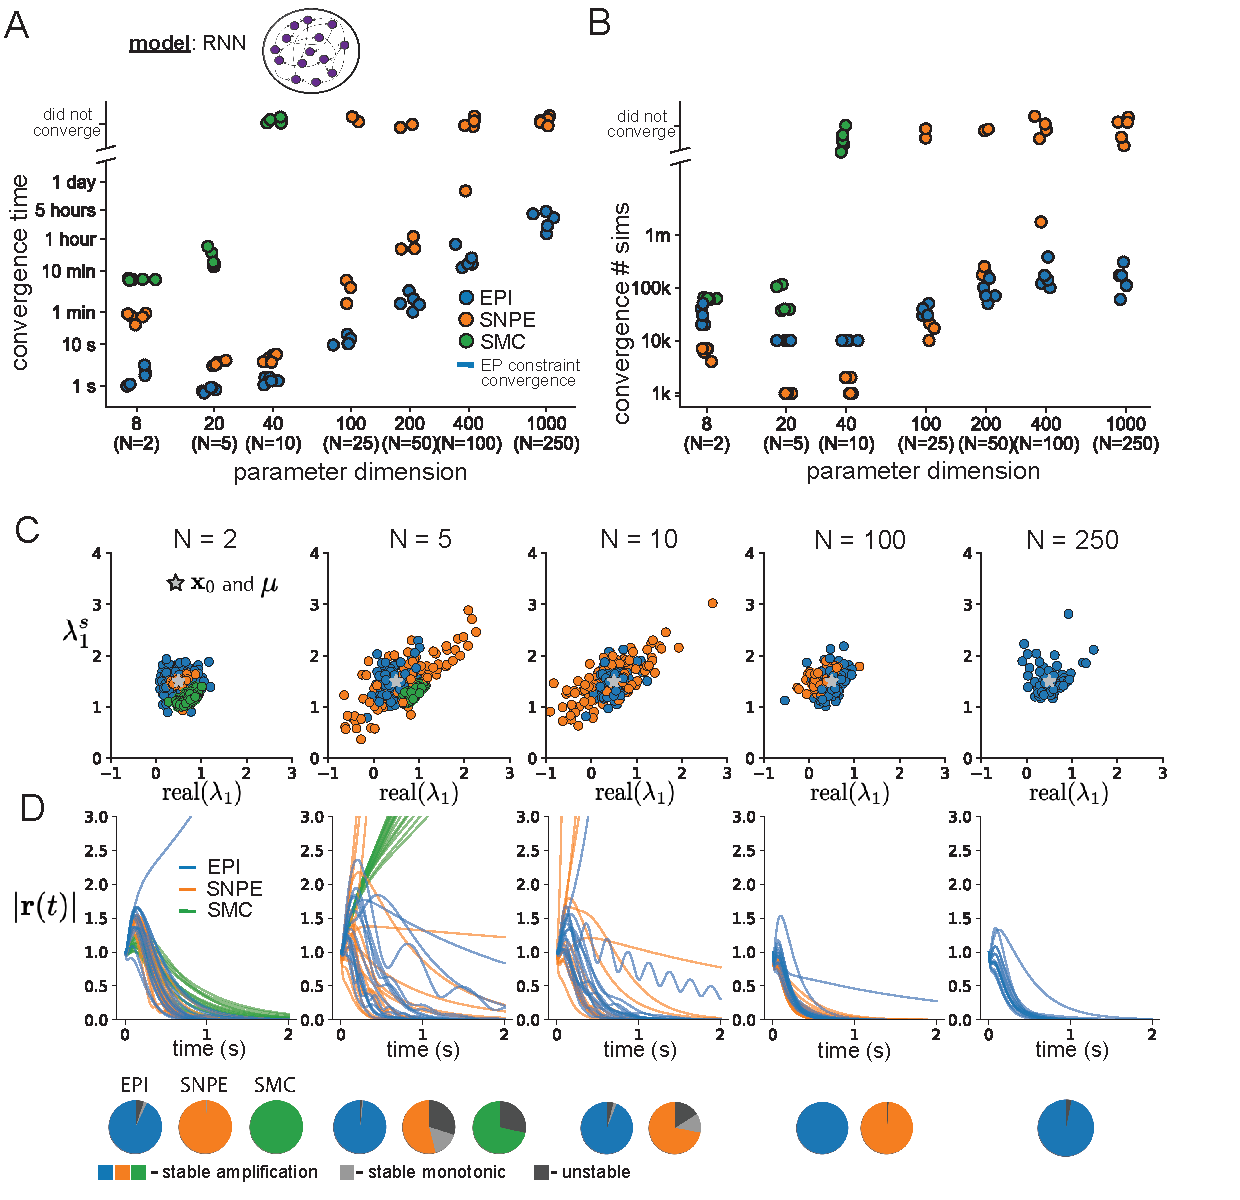
\includegraphics[scale=0.8]{figures/fig2/fig2.pdf}
\end{center}
\vspace{-1cm}
\caption{\small Emergent property inference in the stochastic stabilized supralinear network (SSSN)
\textbf{A}.  Four-population model of primary visual cortex with excitatory (black), parvalbumin (blue), somatostatin (red), and VIP (green) neurons (excitatory and inhibitory projections filled and unfilled, respectively).   
Some neuron-types largely do not form synaptic projections to others ($|W_{\alpha_1, \alpha_2})| < 0.025$).
Each neural population receives a baseline input $\mathbf{h}_b$, and the E- and P-populations also receive a contrast-dependent input $\mathbf{h}_c$.
Additionally, each neural population receives a slow noisy input $\bm{\epsilon}$.
\textbf{B}. Steady-state responses of the SSN model (deterministic, $\bm{\sigma}=\bm{0}$) to varying contrasts.  The response at 50\% contrast (dots) is the focus of our analysis.
\textbf{C}. Transient network responses of the SSSN model at 50 \% contrast. (Left) Traces are independent trials with varying initialization $\mathbf{x}(0)$ and noise realization. (Right) Mean (solid line) and standard deviation (shading) of responses.
\textbf{D}. EPI posterior of noise parameters $\mathbf{z}$ conditioned on E-population variability.
The posterior predictive distribution of $s_E(\mathbf{x}; \mathbf{z})$ is show on the bottom-left.
\textbf{E}. (Top) Enlarged visualization of the $\sigma_E$-$\sigma_P$ marginal distribution of the posteriors $q_{\bm{\theta}}(\mathbf{z} \mid \mathcal{X}(5\text{ Hz})$ and $q_{\bm{\theta}}(\mathbf{z} \mid \mathcal{X}(10\text{ Hz})$.
Each black dot shows the mode at each $\sigma_P$.
The arrows show the most sensitive dimensions of the Hessian evaluated at these modes.
\textbf{F}. The predictive distributions of $\sigma_E^2 + \sigma_P^2$ of each posterior $q_{\bm{\theta}}(\mathbf{z} \mid \mathcal{X}(5\text{ Hz})$ and $q_{\bm{\theta}}(\mathbf{z} \mid \mathcal{X}(10\text{ Hz})$.
}
 \label{fig:V1}
\end{figure}

Dynamical models of excitatory (E) and inhibitory (I) populations with supralinear input-output function have succeeded in explaining a host of experimentally documented phenomena.
In a regime characterized by inhibitory stabilization of strong recurrent excitation, these models give rise to paradoxical responses \cite{tsodyks1997paradoxical}, selective amplification  \cite{goldman2009memory, murphy2009balanced}, surround suppression \cite{ozeki2009inhibitory} and normalization \cite{rubin2015stabilized}. 
Despite their strong predictive power, E-I circuit models rely on the assumption that inhibition can be studied as an indivisible unit. 
However, experimental evidence shows that inhibition is composed of distinct elements -- parvalbumin (P), somatostatin (S), VIP (V) --
composing 80\% of GABAergic interneurons in V1 \cite{markram2004interneurons, rudy2011three, tremblay2016}, and that these inhibitory cell types follow specific connectivity patterns (Fig. \ref{fig:V1}A) \cite{pfeffer2013inhibition}.
Recent theoretical advances \cite{litwin2016inhibitory, GarciaDelMolino2017, Chen2019},  have only started to address the consequences of this multiplicity in the dynamics of V1, strongly relying on linear theoretical tools. 
Here, we use EPI to analyze V1 models of greater complexity in order to characterize properties of slow noise governing circuit variability.

We considered the response properties of a nonlinear dynamical V1 circuit model (Fig. \ref{fig:V1}A) with a state comprised of each neuron-type population's rate $\mathbf{x} = \left[x_E, x_P , x_S, x_V \right]^\top$.
Each population receives recurrent input $W \mathbf{x}$ from synaptic projections of effective connectivity $W$ and an external input $\mathbf{h}$, which determine the population rate via supralinear nonlinearity $\phi = \left[\right]^2_+$.
The input is also comprised of a slow noise component $\bm{\epsilon} \sim OU\left(\tau_{\text{noise}}, \Sigma \right)$ of time scale $\tau_{\text{noise}} > \tau$ and covariance $\Sigma = \text{diag}\left(\bm{\sigma^2}\right)$ (see Section \ref{methods_V1})
\begin{equation}
    \tau \frac{d\mathbf{x}}{dt} = -\mathbf{x} +\phi(W\mathbf{x} + \mathbf{h} + \bm{\epsilon}).
\end{equation}
This model is the stochastic stabilized supralinear network (SSSN) \cite{hennequin2018dynamical} generalized to have inhibitory multiplicity, and introduces stochasticity to previous four neuron-type models of V1 \cite{litwin2016inhibitory}.
Both modeling advancements introduce substantial complexity to mathematical derivations (see Section \ref{methods_V1_complexity}) motivating the treatment of this model with EPI.
Here, we consider fixed weights $W$ and input $\mathbf{h}$ according to a fit of the deterministic model to contrast responses \cite{palmigiano2020structure} (Fig. \ref{fig:V1}B), and study the effect of noise parameterization $\mathbf{z} = [\sigma_E, \sigma_P, \sigma_S, \sigma_V]^\top$ on fluctuations at 50\% contrast. 

For this SSSN, we are interested in how noise variability across neural populations governs stochastic fluctuations in the E-population.
Here, we quantify different levels $y$ of E-population variability with the emergent property
\begin{equation}\label{eq:EP_V1}
\begin{split}
\mathcal{X}(y) ~~:~~  \mathbb{E}_{\mathbf{z}}\begin{bmatrix} s_E(\mathbf{x}; \mathbf{z}) \end{bmatrix}  &~~=~~ y \\ 
 \text{Var}_{\mathbf{z}}\begin{bmatrix} s_E(\mathbf{x}; \mathbf{z}) \end{bmatrix}  &~~=~~  1 \text{Hz}^2,
\end{split}
\end{equation}
where $s_E(\mathbf{x}; \mathbf{z})$ is the standard deviation of the stochastic $E$-population response about its steady state (Fig. \ref{fig:V1}C).

We ran EPI to obtain a posterior distribution $q_{\bm{\theta}}(\mathbf{z} \mid \mathcal{X}(5\text{ Hz})$ producing E-population variability around 5 Hz (Fig. \ref{fig:V1}D).
From the marginal distribution of $\sigma_E$ and $\sigma_P$ (Fig. \ref{fig:V1}D, top-left), we can see that $s_E(\mathbf{x}; \mathbf{z})$ is sensitive to various combinations of $\sigma_E$ and $\sigma_P$.
Alternatively, both $\sigma_S$ and $\sigma_V$ are degenerate with respect to $s_E(\mathbf{x}; \mathbf{z})$ evidenced by the high variability in those dimensions of the posterior (Fig. \ref{fig:V1}D, bottom-right).
Together, these observations imply a parametric manifold of degeneracy with respect to $s_E(\mathbf{x}; \mathbf{z})$ of 5 Hz, which is indicated by the modes along $\sigma_P$ in the $\sigma_E$-$\sigma_P$ marginal (Fig. \ref{fig:V1}E).
The dimensions of sensitivity conferred by EPI and this plain visual structure suggest a quadratic relationship in the emergent property statistic $s_E(\mathbf{x}; \mathbf{z})$ and parameters $\mathbf{z}$, which is preserved at a greater level of variability $\mathcal{X}(10\text{ Hz})$ (Fig. \ref{fig:V1}E).
Indeed, the sum of squares of $\sigma_E$ and $\sigma_P$ is larger in $q_{\bm{\theta}}(\mathbf{z} \mid \mathcal{X}(10\text{ Hz})$ than $q_{\bm{\theta}}(\mathbf{z} \mid \mathcal{X}(5\text{ Hz})$ (Fig \ref{fig:V1}F, $p=0$), while the sum of squares of $\sigma_S$ and $\sigma_V$ are not significantly different in the two posteriors (Fig. \ref{fig:V1_3}, $p=.402$).

While a quadratic relationship in $s_E(\mathbf{x}; \mathbf{z})$ and $\mathbf{z}$ is potentially derivable by extending the derivation in Section \ref{methods_V1} to the case of $\tau \neq \tau_{\text{noise}}$, the coefficients in front of each quadratic term would be unruly, and likely escape comprehensible analysis.
This makes EPI an attractive tool for revealing the characteristics of noise governing variability and for answering other questions in this complex model.
Intriguingly, this circuit exhibited a paradoxical effect in the P-population, and no other inhibitory types at 50\% contrast (Fig. \ref{fig:V1_3}) implying that the E-population is P-stabilized.
Future work motivated by our analysis here, may uncover a relationship between the neuron-type mediating stability and the factors governing circuit variability.


%%%%%%%%%%%%%%%%%%%%%%%%
\subsection{EPI identifies multiple regimes of rapid task switching} \label{results_SC}
%In a rapid task switching experiment \cite{duan2015requirement}, rats were explicitly cued on each trial to either orient towards a visual stimulus in the Pro (P) task or orient away from a visual stimulus in the Anti (A) task (Fig. \ref{fig:SC}a). 
%Neural recordings in the midbrain superior colliculus (SC) exhibited two populations of neurons that simultaneously represented both task context (Pro or Anti) and motor response (contralateral or ipsilateral to the recorded side): the Pro/Contra and Anti/Ipsi neurons \cite{duan2018collicular}.
%Duan et al. proposed a model of SC that, like the V1 model analyzed in the previous section, is a four-population dynamical system.  
%We analyzed this model, where the neuron-type populations are functionally-defined as the Pro- and Anti-populations in each hemisphere (left (L) and right (R)), their connectivity is parameterized geometrically  (Fig. \ref{fig:SC}B).
%The input-output function of this model is chosen such that the population responses $x = [x_{LP}, x_{LA}, x_{RP}, x_{RA}]^\top$ are bounded from 0 to 1 giving rise to high (1) or low (0) responses at the end of the trial:
%\begin{equation}
%x_\alpha =\left(\frac{1}{2}\tanh\left(\frac{u_\alpha - \epsilon}{\zeta}\right)+ \frac{1}{2} \right)
%\end{equation}
%where $\epsilon = 0.05$ and $\zeta = 0.5$.  
%The dynamics evolve with timescale $\tau=0.09$ via an internal variable $u$ governed by connectivity weights $W$
%\begin{equation}
%\tau \frac{du}{dt} = -u + Wx + h + \sigma dB
%\end{equation}
%with gaussian noise of variance $\sigma^2$ = 1.
%The input $h$ is comprised of a cue-dependent input to the Pro or Anti populations, a stimulus orientation input to either the Left or Right populations, and a choice-period input to the entire network (see Section \ref{methods_SC}).
%Here, we use EPI to determine the changes in network connectivity $z = [ sW_P, sW_A, vW_{PA}, vW_{AP}, dW_{PA}, dW_{AP}, hW_P, hW_A]$ resulting in greater levels of rapid task switching accuracy.
%
%\begin{figure}
%\begin{center}
%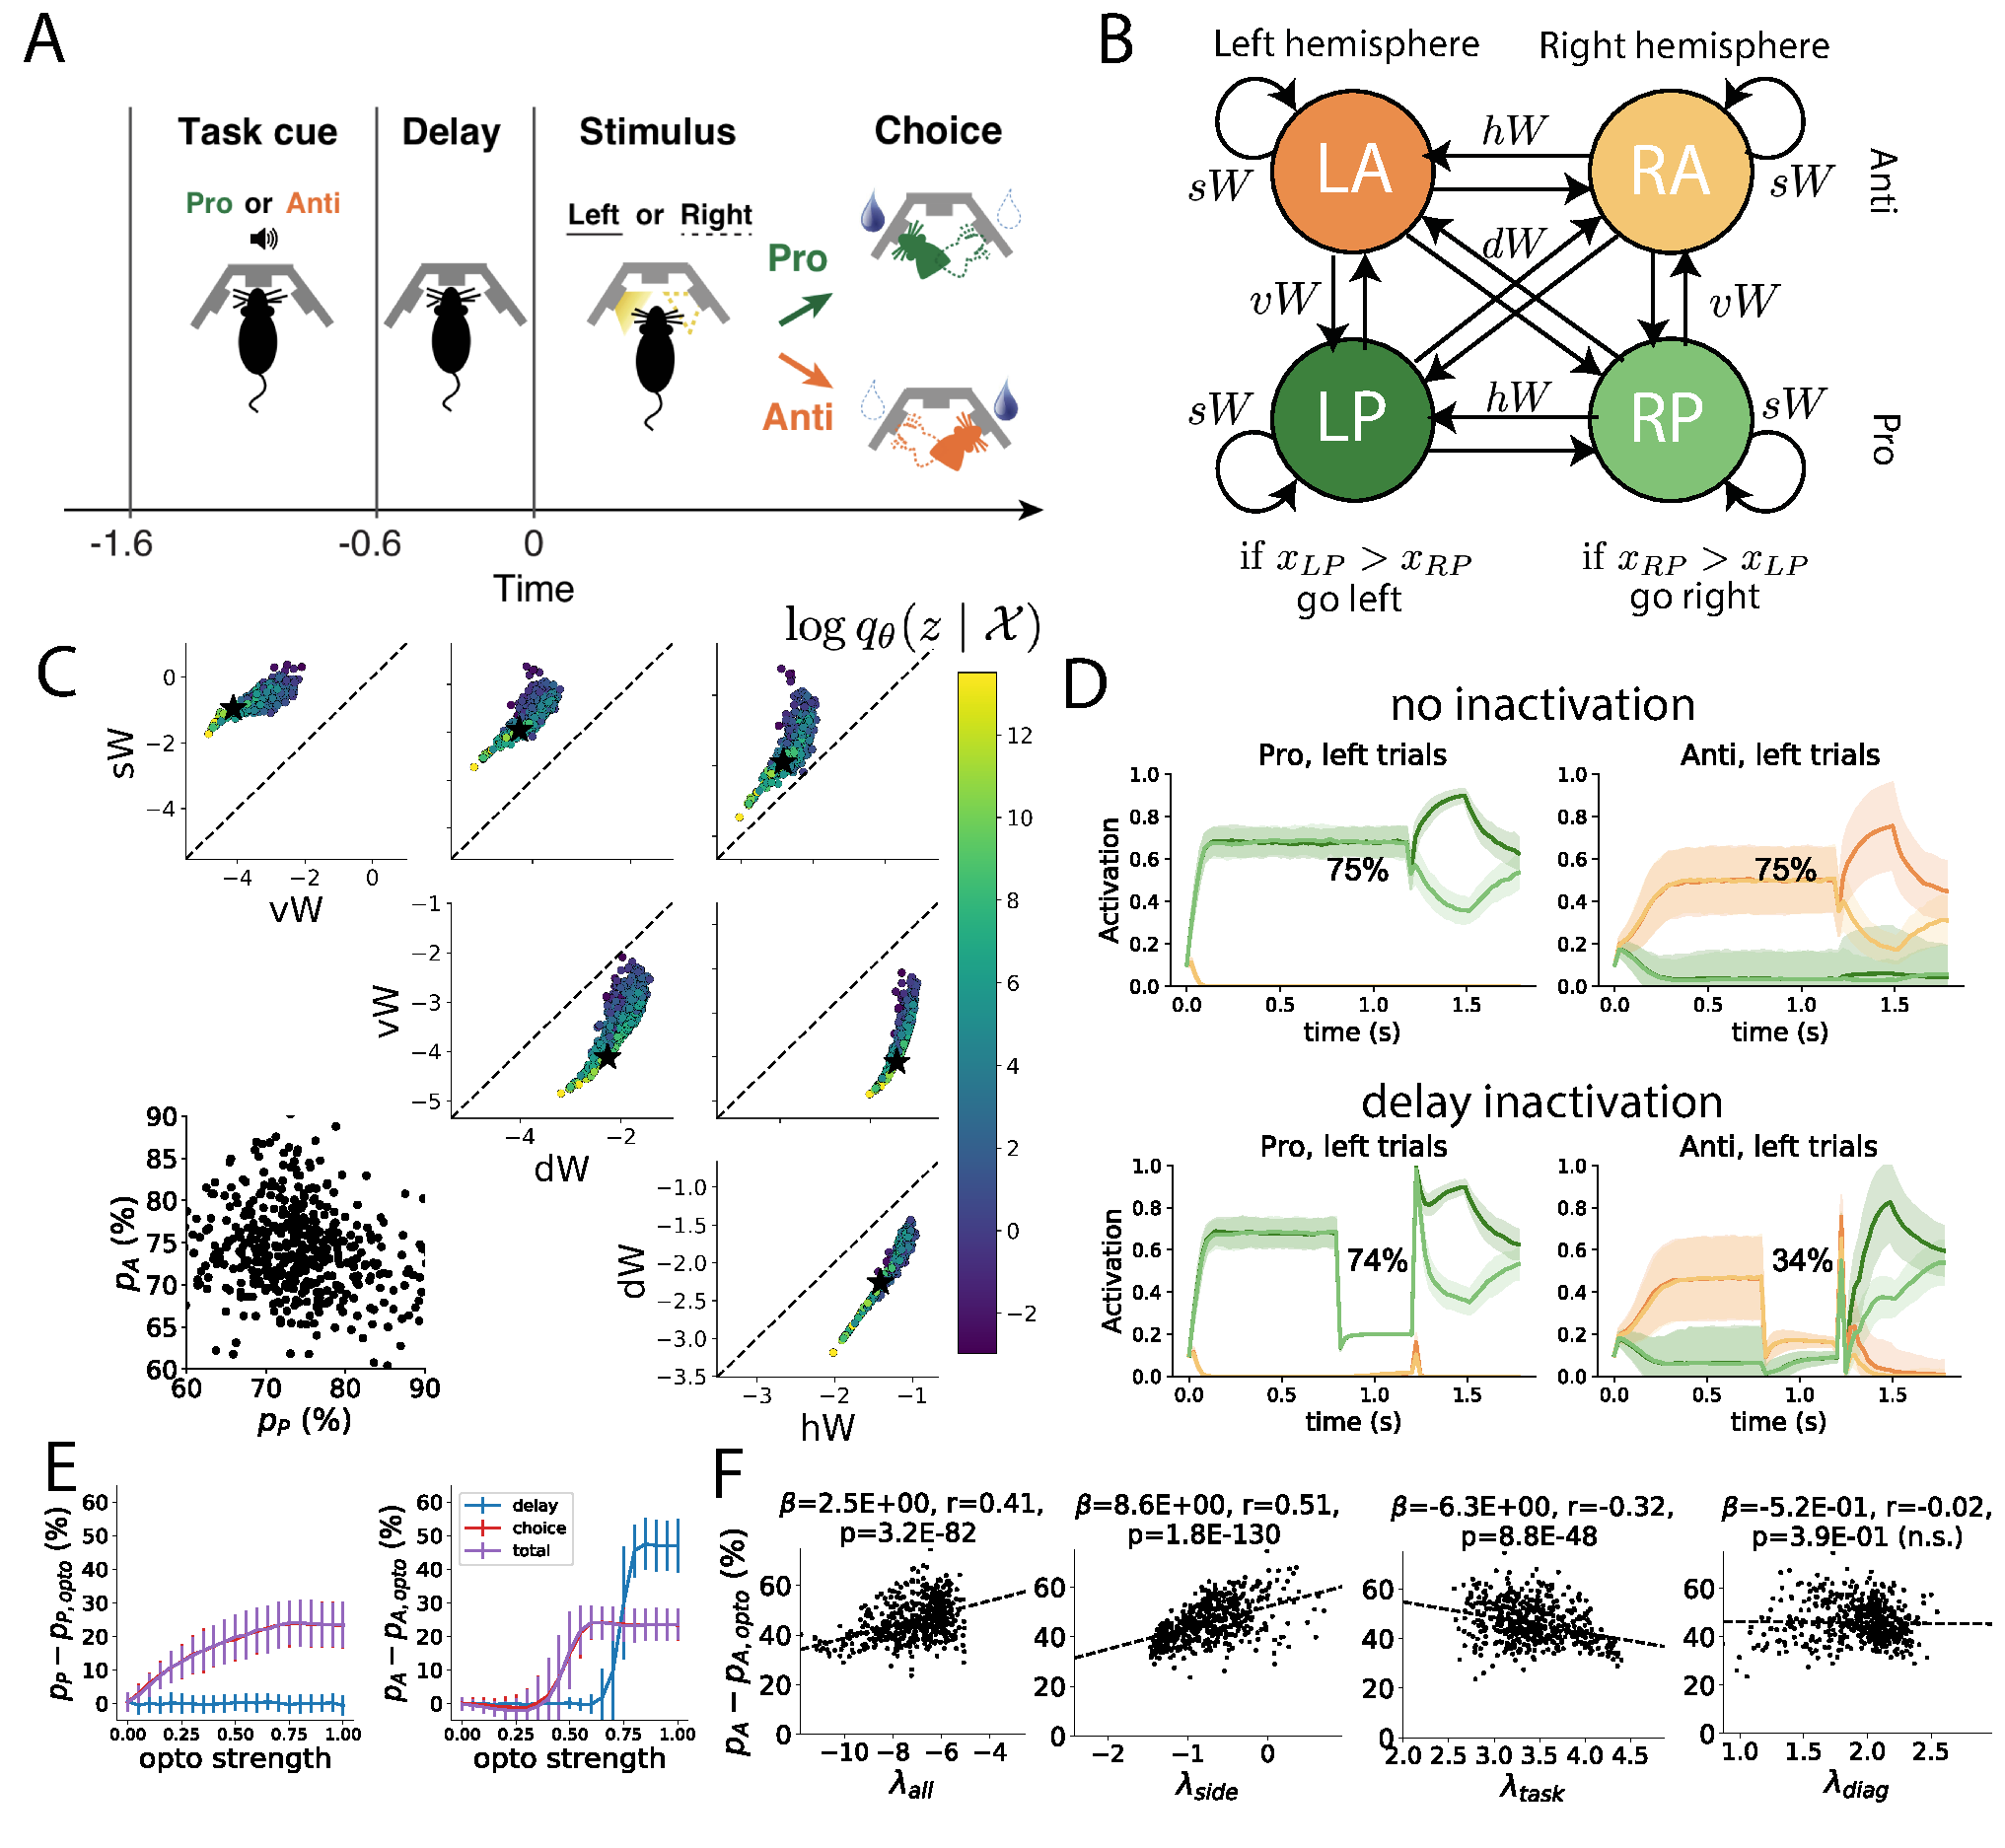
\includegraphics[scale=0.5]{figures/fig4/fig4.pdf}
%\end{center}
%\caption{\small EPI reveals changes in SC \cite{duan2018collicular} connectivity that control task accuracy.  
%A. Rapid task switching behavioral paradigm (see text). 
%B. Model of superior colliculus (SC). Neurons: LP - left pro, RP - right pro, LA - left anti, RA - right anti. 
%Parameters: $sW$ - self, $hW$ - horizontal, $vW$ -vertical, $dW$ - diagonal weights.  
%Subscripts $P$ and $A$ of connectivity weights indicate Pro or Anti populations, and e.g. $vW_{PA}$ is a vertical weight from an Anti to a Pro population.  
%C. The Schur decomposition of the weight matrix $W = V\Lambda V^{-1}$ is a unique decomposition with orthogonal $V$ and upper triangular $\Lambda$. Schur modes: $v_{\text{all}}$, $v_{\text{task}}$, $v_{\text{side}}$, and $v_{\text{diag}}$.  
%D. The marginal EPI distributions of the Schur eigenvalues at each level of task accuracy.
%E. The correlation of Schur eigenvalue with task performance in each learned EPI distribution.}
%\label{fig:SC}
%\end{figure}
%
%To quantify the emergent property of rapid task switching at various levels of accuracy, we considered the requirements of this model in this behavioral paradigm.
%At the end of successful trials, the response of the Pro population in the hemisphere of the correct choice must have a value near 1, while the Pro population in the opposite hemisphere must have a value near 0.
%Constraining a population response $x_\alpha \in \left[0,1\right]$ to be either 0 or 1 can be achieved by requiring that it has Bernoulli variance (see Section \ref{methods_SC}).
%Thus, we can formulate rapid task switching at a level of accuracy $p \in \left[0, 1\right]$ in both tasks in terms of the average steady response of the Pro population $\hat{p}$ of the correct choice,  the error in Bernoulli variance of that Pro neuron $\sigma^2_{\text{err}}$, and the average difference in Pro neuron responses $d$ in both Pro and Anti trials:
%\begin{equation}
%\mathcal{B}(p) ~~\triangleq~~ \mathbb{E}\begin{bmatrix} \hat{p}_P \\ \hat{p}_A \\ (\hat{p}_P-p)^2 \\ (\hat{p}_A - p)^2 \\ \sigma^2_{P,err} \\ \sigma^2_{A,err} \\ d_P \\ d_A \end{bmatrix} = \begin{bmatrix} p \\ p \\ 0.15^2 \\ 0.15^2 \\ 0 \\ 0 \\ 1 \\ 1 \end{bmatrix}.
%\end{equation}
%Thus, $\mathcal{B}(p)$ denotes Bernoulli, winner-take-all responses between Pro neurons in a model executing rapid task switching near accuracy level $p$.
%
%We used EPI to learn distributions of the SC weight matrix parameters $z$ conditioned on of various levels of rapid task switching accuracy $\mathcal{B}(p)$ for $p \in \{50\%, 60\%, 70\%, 80\%, 90\%\}$.
%To make sense of these inferred distributions, we followed the approach of Duan et al. by decomposing the connectivity matrix $W = V\Lambda V^{-1}$ in such a way (the Schur decomposition) that the basis vectors $v_i$ are the same for all $W$ (Fig. \ref{fig:SC}C). 
%These basis vectors have intuitive roles in processing for this task, and are accordingly named the \textit{all} mode - all neurons co-fluctuate, \textit{side} mode - one side dominates the other, \textit{task} mode - the Pro or Anti populations dominate the other, and \textit{diag} mode - Pro- and Anti-populations of opposite hemispheres dominate the opposite pair. 
%The corresponding eigenvalues (e.g. $\lambda_{\text{task}}$, which change according to $W$) indicate the degree to which activity along that mode is increased or decreased by $W$. 
%
%We found that for greater task accuracies, the task mode eigenvalue increases, indicating the importance of $W$ to the task representation (Fig. \ref{fig:SC}D, purple; adjacent distributions from 60\% to 90\% have  $p<10^{-4}$, Mann-Whitney test with 50 estimates and 100 samples).
%Stepping from random chance (50\%) networks to marginally task-performing (60\%) networks, there is a marked decrease of the side mode eigenvalues (Fig. \ref{fig:SC}D, orange; $p<10^{-4}$).  
%Such side mode suppression relative to $50\%$ remains in the models achieving greater accuracy, revealing its importance towards task performance.
%There were no interesting trends with task accuracy in the all or diag mode (hence not shown in Fig. \ref{fig:SC}). 
%Importantly, we can conclude from our methodology that side mode suppression in $W$ allows rapid task switching, and that greater task-mode representations in $W$ increase accuracy.  
%These hypotheses are confirmed by forward simulation of the SC model (Fig. \ref{fig:SC}E, see Section \ref{methods_SC}) suggesting experimentally testable predictions: increase in rapid task switching performance should be correlated with changes in effective connectivity corresponding to an increase in task mode and decrease in side mode eigenvalues.

In a rapid task switching experiment \cite{duan2015requirement}, rats were explicitly cued on each trial to either orient towards a visual stimulus in the Pro (P) task or orient away from a visual stimulus in the Anti (A) task (Fig. \ref{fig:SC}A). 
Neural recordings in the midbrain superior colliculus (SC) exhibited two populations of neurons that simultaneously represented both task context (Pro or Anti) and motor response (contralateral or ipsilateral to the recorded side): the Pro/Contra and Anti/Ipsi neurons \cite{duan2018collicular}.
Duan et al. proposed a model of SC that, like the V1 model analyzed in the previous section, is a four-population dynamical system.  
We analyzed this model, where the neuron-type populations are functionally-defined as the Pro- and Anti-populations in each hemisphere (left (L) and right (R)), their connectivity is parameterized geometrically  (Fig. \ref{fig:SC}B).
The input-output function of this model is chosen such that the population responses $\mathbf{x} = [x_{LP}, x_{LA}, x_{RP}, x_{RA}]^\top$ are bounded from 0 to 1 as a function $\phi$ of a dynamically evolving internal variable $\mathbf{u}$.
The model responds to the side with greater Pro neuron activation; e.g. the response is left if $x_{LP} > x_{RP}$ at the end of the trial.
The dynamics evolve with timescale $\tau= 90\text{ms}$ governed by connectivity weights $W$
\begin{equation}
\begin{split}
\tau \frac{d\mathbf{u}}{dt} &= -\mathbf{u} + W\mathbf{x} + \mathbf{h} + d\mathbf{B} \\
\mathbf{x} &= \phi(\mathbf{u})
\end{split}
\end{equation}
with white noise of variance $0.2^2$.
The input $\mathbf{h}$ is comprised of a cue-dependent input to the Pro or Anti populations, a stimulus orientation input to either the Left or Right populations, and a choice-period input to the entire network (see Section \ref{methods_SC}).
Here, we use EPI to determine the changes in network connectivity $\mathbf{z} = [sW, vW, dW, hW]^{\top}$ resulting in execution of rapid task switching behavior.

\begin{figure}
\begin{center}
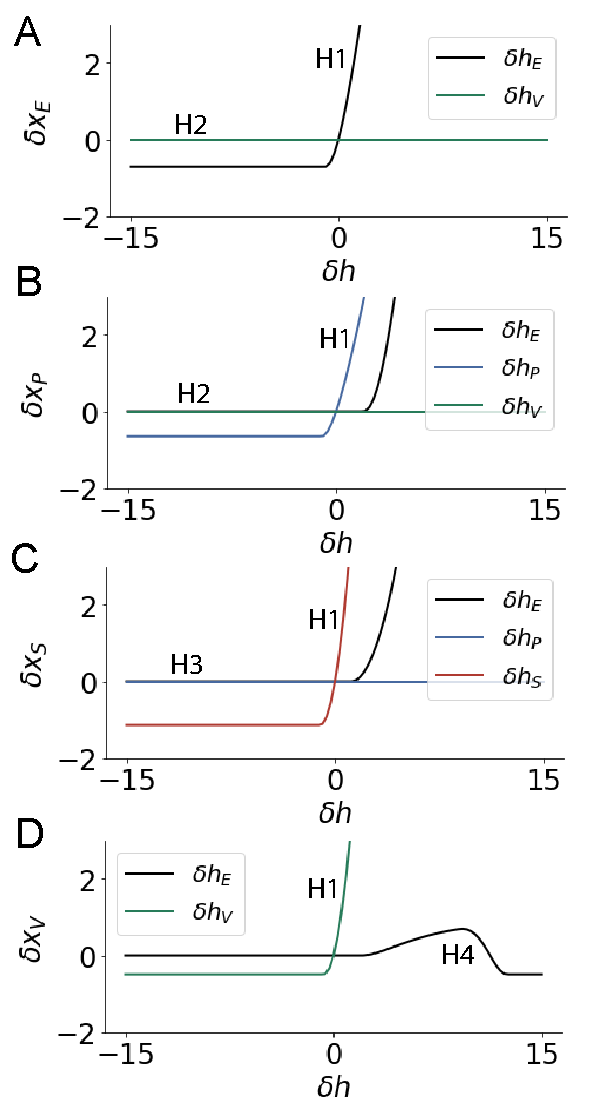
\includegraphics[scale=0.8]{figures/fig3/fig3.pdf}
\end{center}
\caption{\footnotesize 
\textbf{A}. Rapid task switching behavioral paradigm (see text). 
\textbf{B}. Model of superior colliculus (SC). Neurons: LP - left pro, RP - right pro, LA - left anti, RA - right anti. 
Parameters: $sW$ - self, $hW$ - horizontal, $vW$ -vertical, $dW$ - diagonal weights.  
\textbf{C}. The EPI posterior distribution of rapid task switching networks.  
Red and purple stars ($\mathbf{z}_1$ and $\mathbf{z}_2$) indicate different connectivity regimes with different sensitivity vectors $\mathbf{v}_1$ and $\mathbf{v}_2$.
(Middle-left) Posterior predictive distribution of task accuracies.
(Bottom-left) Task accuracy along dimensions of sensitivity in each connectivity regime.
\textbf{D}. Means (solid) and standard deviations (shaded) of each population across random simulated trials.
Top plots show Pro (top) and Anti (bottom) responses for connectivity $\mathbf{z}_1$.
Bottom rows show the same $\mathbf{z}_2$.
\textbf{E}. The EPI posterior predicts experimental results (left) showing no change in the Pro task, but larger error in the Anti task (right).
\textbf{F}. Accuracy in the Anti task during delay period optogenetic inactivation $p_{A,\text{opto}}$ is strongly anticorrelated with accuracy in the Pro task.
\textbf{G}. Accuracy with delay period inactivation along each connectivity regime's dimension of sensitivity.
}
\label{fig:SC}
\end{figure}

We define rapid task switching behavior as accurate execution of each task.  Inferred models should not exhibit fully random responses (50\%), or perfect performance (100\%), since perfection is never attained by even the best trained rats.
We formulate rapid task switching as an emergent property by stipulating that the average accuracy in the Pro task $p_P(\mathbf{x}; \mathbf{z})$ and Anti task $p_A(\mathbf{x}; \mathbf{z})$ be $75\%$ with variance $7.5\%^2$.
\begin{equation}\label{eq:SC_EP}
\begin{split}
\mathcal{X} ~~:~~ \mathbb{E}_{\mathbf{z}}\begin{bmatrix} p_P(\mathbf{x}; \mathbf{z}) \\ p_A(\mathbf{x}; \mathbf{z}) \end{bmatrix}  &~~=~~  \begin{bmatrix} 75\% \\ 75\% \end{bmatrix}  \\ 
 \text{Var}_{\mathbf{z}}\begin{bmatrix} p_P(\mathbf{x}; \mathbf{z}) \\ p_A(\mathbf{x}; \mathbf{z}) \end{bmatrix}  &~~=~~  \begin{bmatrix} 7.5\%^2 \\ 7.5\%^2  \end{bmatrix}
\end{split}
\end{equation}
A variance of $7.5\%^2$  in each task will confer a posterior producing performances ranging from about $60\%-90\%$, allowing us to examine the properties of connectivity that yield better performance in each task.
Notably, this is our first example using EPI to condition on multiple emergent property statistics ($|f(\mathbf{x}; \mathbf{z})| = 2$).

We ran EPI to obtain the posterior connectivities $\mathbf{z}$ producing rapid task switching (Fig. \ref{fig:SC}C).
The inferred parameters generate a distribution of task accuracies (Fig. \ref{fig:SC}C, middle-left) according to our mathematical definition of rapid task switching (Equation \ref{eq:SC_EP}).
The nonlinear patterns of connectivity that govern each task accuracy (Fig. \ref{fig:SC1}A-B) are not fully captured by linear prediction (Fig. \ref{fig:SC1}C).
For example, the patterns in connectivity increasing Pro accuracy change dramatically after crossing a threshold of $sW$ (Fig. \ref{fig:SC1}A $sW$-$hW$ marginal).
Not only has EPI captured this complex nonlinear posterior, it offers probabilistic tools for understanding the different regimes of model behavior.

To establish these two regimes of connectivity, we took gradient steps along $q_{\bm{\theta}}(\mathbf{z} \mid \mathcal{X})$to produce modes $\mathbf{z}_1$ and $\mathbf{z}_2$  (Fig. \ref{fig:SC}C red and purple stars, Section \ref{methods_SC}).
Simulations from these two regimes reveal different responses in each task (Fig. \ref{fig:SC}D).
We charcaterized these regimes by identifying the dimensions of connectivity that rapid task switching is most sensitive to.
The sensitivity dimensions $\mathbf{v}_1$ and  $\mathbf{v}_2$ (Fig. \ref{fig:SC}C, red and purple arrows) point in different directions, resulting in different changes to task accuracy (Fig. \ref{fig:SC}D, bottom-left, \ref{fig:SC2}).
In regime 1, Anti accuracy diminishes in either direction of sensitivity away from the mode, while in regime 2, Anti accuracy tracks monotonic increases in Pro accuracy.
These responses make intuitive sense, recognizing that $\mathbf{v}_1$ (unlike $\mathbf{v}_2$) points strongly in the direction of connectivity eigenvalue $\lambda_{\text{diag}}$, which is strongly anticorrelated with $p_A$ (Fig. \ref{fig:SC3}, \ref{fig:SC4}, see Section \ref{methods_SC}).

In agreement with experimental results from Duan et al., we found optogenetic inactivation during the delay period consistently decreased performance in the Anti task, but had no effect on the Pro task (Fig. \ref{fig:SC}E)).
This difference in resiliency across tasks to delay perturbation is a prediction made by the inferred EPI distribution, rather than an emergent property that was conditioned upon.
Similarities across Pro and Anti trials in choice period responses following delay period inactivation (Fig. \ref{fig:SC5}A) suggested that connectivity patterns inducing greater Pro task accuracy increase error in delay period inactivated Anti trials (Fig. \ref{fig:SC}F).
The strong anticorrelation between $p_P$ and $p_{A, opto}$ across posterior connectivities led to the following hypothesis about each connectivity regime: the sensitivity dimension of each regime decreases $p_{A,opto}$ irrespective of its effect $p_A$, since both $\mathbf{v}_1$ and $\mathbf{v}_2$ increase $p_P$.
Indeed, in regimes 1 and 2 whose sensitivity dimension elicits very different responses in $p_A$, $p_{A,opto}$ decreases since the connectivity changes enhancing $p_P$ exacerbate Anti trial error (Fig. \ref{fig:SC}F).

In summary, we used EPI to obtain the full distribution of connectivities that execute rapid task switching.
This posterior revealed multiple regimes of rapid task switching, which we characterized using the probabilistic toolkit EPI seemlessly affords.
EPI allowed us to conclude that since \textit{all} parameters of this model producing rapid task switching make an experimentally verified prediction, we have a well-chosen model in that regard.
Finally, we used our knowledge about how $\mathbf{z}$ governs $p_{A,opto}$ to make accurate predictions about each identified regime of connectivity.

\subsection{EPI scales well to high-dimensional parameter spaces} \label{results_LRRNN}
Here, we study the scalability of EPI in number of parameters $|\mathbf{z}|$ by inferring the connectivities of recurrent neural networks (RNNs, Fig. \ref{fig:LRRNN}A). 
 We consider a rank-2 RNN with N neurons of connectivity
\begin{equation}
 W = UV^\top + g\chi
 \end{equation}
 and dynamics
 \begin{equation}
 \tau \dot{\mathbf{x}} = -\mathbf{x} + W\mathbf{x}
 \end{equation}
where $U = \begin{bmatrix} \mathbf{u}_1 & \mathbf{u}_2 \end{bmatrix}$, $V = \begin{bmatrix} \mathbf{v}_1 & \mathbf{v}_2 \end{bmatrix}$, $\mathbf{u}_1, \mathbf{u}_2, \mathbf{v}_1, \mathbf{v}_2 \in \left[-1, 1 \right]^N$, and $g=0.01$.  We  infer connectivity distributions $\mathbf{z} = \left[\mathbf{u}_1^\top, \mathbf{u}_2^\top, \mathbf{v}_1^\top, \mathbf{v}_2^\top \right]^\top$   producing stable amplification.
RNN's exhibiting stable amplification amplify responses to input along some dimensions, and are stable across all dimensions.
Two conditions are both necessary and sufficient for RNNs to exhibit stable amplification \cite{bondanelli2020coding}:  $\text{real}(\lambda_1) < 1$ and
$\lambda^s_1 > 1$, where $\lambda_1$ is the eigenvalue of $W$ with greatest real part and $\lambda^s$ is the maximum eigenvalue of $W^s = \frac{W + W\top}{2}$.

In our analysis, we seek to condition rank-2 networks of increasing size on a regime of stable amplification.  
Networks with $\text{real}(\lambda_1) = 0.5 \pm 0.5$ and $\lambda_1^s = 1.5 \pm 0.5$ will yield moderate amplification.
 EPI can naturally condition on this emergent property
\begin{equation}\label{eq:EP_LRRNN}
\begin{split}
\mathcal{X} ~~:~~ \mathbb{E}_{\mathbf{z}, \mathbf{x}} \begin{bmatrix} \text{real}(\lambda_1) \\ \lambda^s_1 \end{bmatrix} &= \begin{bmatrix} 0.5 \\ 1.5 \end{bmatrix} \\
\text{Var}_{\mathbf{z}, \mathbf{x}} \begin{bmatrix} \text{real}(\lambda_1) \\ \lambda^s_1 \end{bmatrix} &= \begin{bmatrix} 0.25^2 \\ 0.25^2 \end{bmatrix} .
\end{split}
\end{equation}

For comparison, we infer rank-2 RNN connectivites with alternative approaches to likelihood free inference.
ABC methods define a distance tolerance $\epsilon$ observed data $x_0$ for which we keep sampled parameters.
To make this ABC approach as similar as possible to the EPI program defined by Equation \ref{eq:EP_LRRNN}, we chose $\epsilon = 0.5$, an $l$-$2$ distance metric, and 
\begin{equation}\label{eq:SNPE_stab_amp_x0}
x_0 = \begin{bmatrix} \text{real}(\lambda_1) \\ \lambda^s_1 \end{bmatrix} = \begin{bmatrix} 0.5 \\ 1.5 \end{bmatrix}
\end{equation}
located at the mean of our desired emergent property.
We use sequential Monte Carlo ABC (SMC-ABC), to compare efficiency, since it is considered the state-of-the-art ABC approach.
SNPE \cite{gonccalves2019training} is another deep likelihood-free inference method that emerged along with this work.
In contrast to EPI, SNPE cannot condition on the variance of the posterior predictive distribution. 
Also, there is no tolerance parameter for SNPE like $\epsilon$ in ABC, so the comparative SNPE approach simply conditions on observation $x_0$.

As we scale the number of neurons $N$ in the RNN, and thus the dimensionality of the parameter space $\mathbf{z} \in [-1, 1]^{4N}$, we see that EPI has superior scaling properties (Fig. \ref{fig:LRRNN}B).
SMC-ABC and SNPE become intractable around 25 and 90 dimensions respectively, while EPI can infer 1000-dimensional distributions in about 1 day.
No matter the number of neurons, EPI always produces the same distribution of emergent property statistics $\text{real}(\lambda_1)$ and $\lambda_1^s$ (Fig. \ref{fig:LRRNN}C, blue), and high variation in response profiles \ref{fig:LRRNN}D, red).
For the dimensionalities in which SMC-ABC is tractable, the inferred parameters always exhibit stable amplification, are less varied \ref{fig:LRRNN}C, red) and largely produce similar responses \ref{fig:LRRNN}D, red).
When using SNPE the inferred parameters are widely varied \ref{fig:LRRNN}C, orange), but often produce non amplified or unstable responses \ref{fig:LRRNN}D, orange).
In conclusion, we found that deep likelihood-free inference techniques are capable of scaling to higher dimensional inference than SMC-ABC.
However, only EPI can scale to high dimensions while reproducing the emergent property.


\begin{figure}
\begin{center}
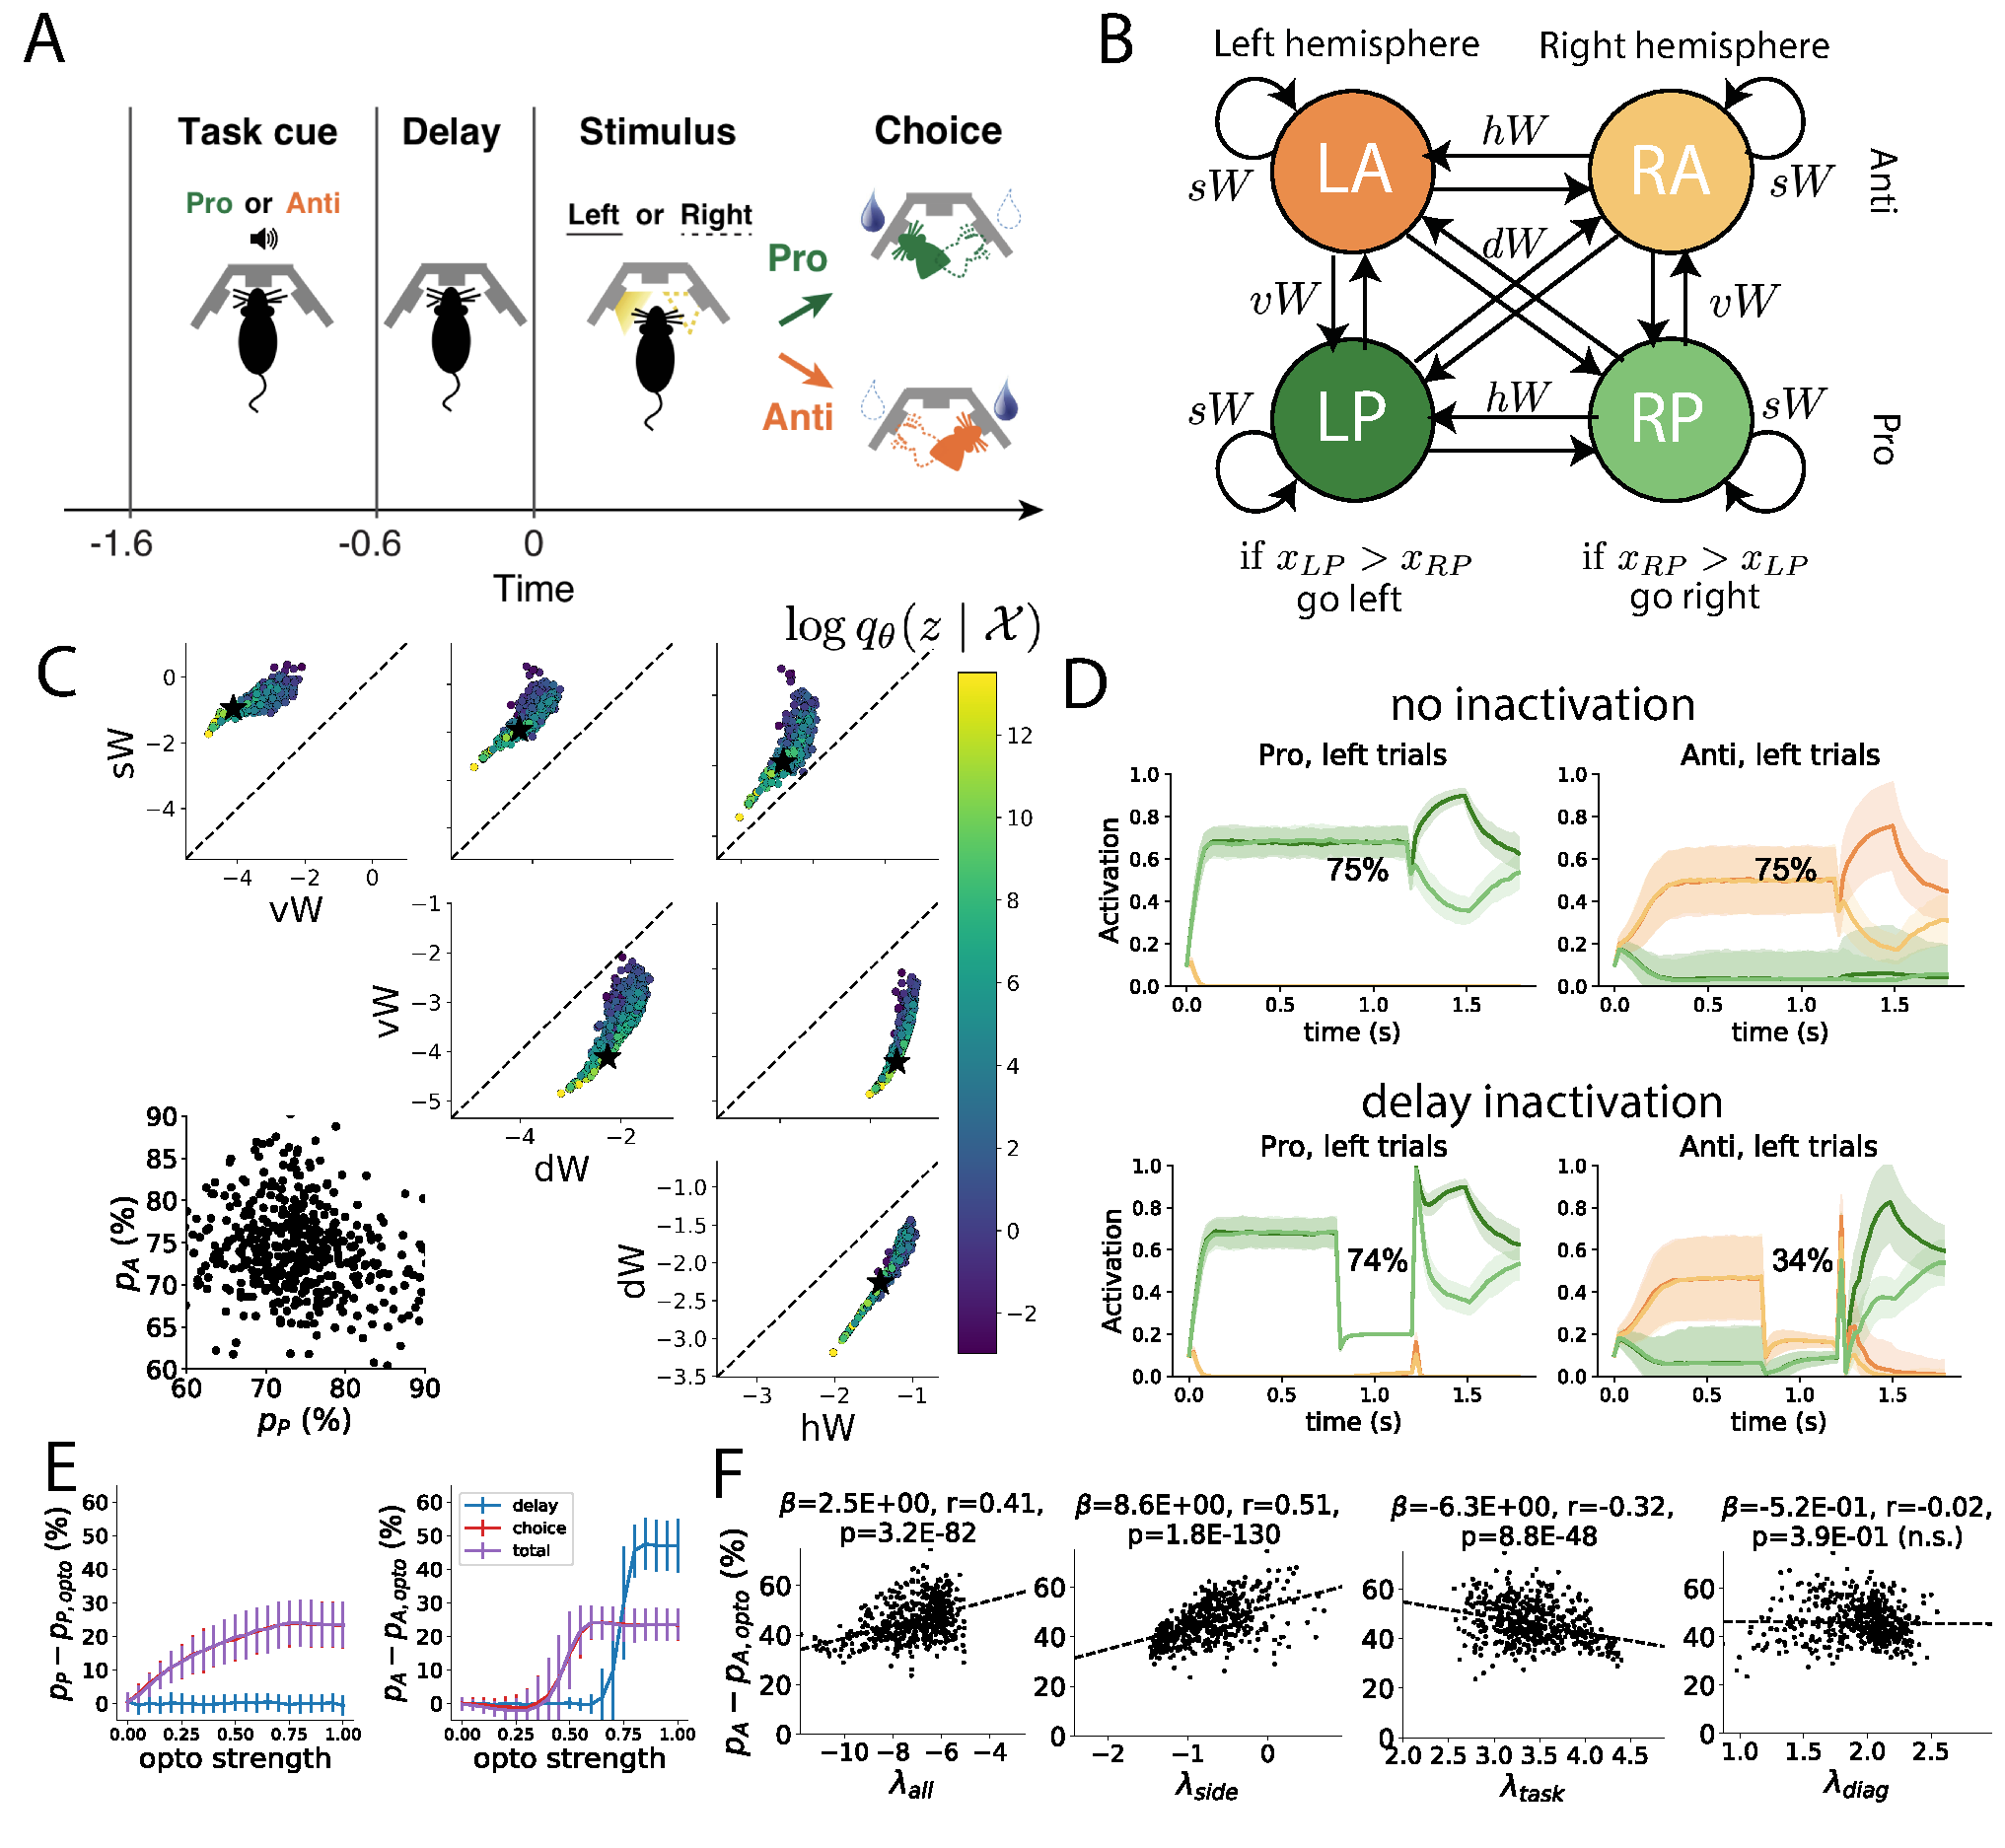
\includegraphics[scale=.8]{figures/fig4/fig4.pdf}
\end{center}
\caption{\small 
\textbf{A}. Recurrent neural network.
\textbf{B}. EPI scales with $z$ to high dimensions. 
Convergence definitions: 
EPI (blue) - satisfies all moment constraints, 
SNPE (orange)- produces at least 2/$n_{\text{train}}$ parameter samples are in the bounds of emergent property (mean +- 0.5), 
and SMC-ABC (red) - 100 particles with $\epsilon < 0.5$ are produced.
\textbf{C}. Posterior predictive distributions of EPI (blue), SNPE (orange), and SMC-ABC (red). 
Gray star indicates emergent property mean, and gray dashed lines indicate two standard deviations corresponding to the variance constraint.
For $N <= 6$ where SMC-ABC converges, samples are not diverse (path degeneracies).  
For $N >= 25$, SNPE does not produce a posterior approximation yielding parameters with simulations near $x_0$. 
\textbf{D}. Simulations of network parameters resulting from each method ($\tau=100ms$).  Each trace corresponds to simulation of one $z$.  
\textbf{E}. Ratio of obtained samples producing stable amplification.
}
\label{fig:LRRNN}
\end{figure}

%%%%%%%%%%%%%%%%%%%%%%%%
%\subsection{Linking RNN connectivity to error} \label{results_RNN}
%So far, each model we have studied was designed from fundamental biophysical principles, genetically- or functionally-defined neuron types.  
%At a more abstract level of modeling, recurrent neural networks (RNNs) are high-dimensional dynamical models of computation that are becoming increasingly popular in neuroscience research \cite{barak2017recurrent}. 
%In theoretical neuroscience, RNN dynamics usually follow the equation
%\begin{equation}
%\frac{dx}{dt} = -x + W \phi(x) + h,
%\end{equation}
%where $x$ is the network activity, $W$ is the network connectivity, $\phi(\cdot) = \tanh(\cdot)$, and $h$ is the input to the system.
%Such RNNs are trained to do a task from a systems neuroscience experiment, and then the unit activations of the trained RNN are compared to recorded neural activity.
%Fully-connected RNNs with tens of thousands of parameters are challenging to characterize \cite{sussillo2013opening}, especially making statistical inferences about their parameterization.
%Alternatively, we considered a rank-1, $N$-neuron RNN with connectivity consisting of the sum of a random and a structured component:
%\begin{equation}
%W = g\chi + \frac{1}{N}mn^\top.
%\end{equation}
%The random component $g \chi$ has strength $g$, and random component weights are Gaussian distributed $\chi_{i,j} \sim \mathcal{N}(0, \frac{1}{N})$.  
%The structured component $\frac{1}{N}m n\top$ has entries of $m$ and $n$ drawn from Gaussian distributions $m_i \sim \mathcal{N}(M_m, 1)$ and $n_i \sim \mathcal{N}(M_n, 1)$.
%Recent theoretical work derives the low-dimensional response properties of low-rank networks from statistical parameterizations of their connectivity, such as $z = [g, M_m, M_n]$ \cite{mastrogiuseppe2018linking}.
%We used EPI to infer the parameterizations of rank-1 RNNs solving an example task, enabling discovery of properties of connectivity that result in different types of error in the computation.
%
%\begin{figure}
%\begin{center}
%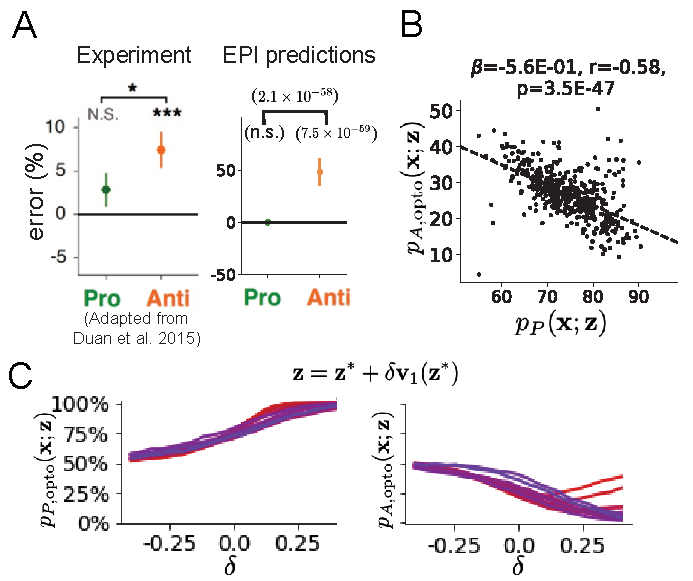
\includegraphics[scale=0.75]{figures/fig5/fig5.pdf}
%\end{center}
%\caption{\small Sources of error in an RNN solving a simple task.  A. (left) A rank-1 RNN executing a Gaussian posterior conditioning computation on $\mu_y$. 
%(right) Error in this computation can come from over- or under-estimating the posterior mean or variance. 
%B. EPI distribution of rank-1 RNNs executing Gaussian posterior conditioning.  Samples are colored by (left) posterior mean $\mu_{\text{post}}=\kappa_r$ and (right) posterior variance $\sigma^2_{\text{post}}=\Delta_T$  
%C.  Finite-size network simulations of 2,000 neurons with parameters $z_1$ and $z_2$ sampled from the inferred distribution.  
%Activity along readout $\kappa_r$ (cyan) is stable despite chaotic fluctuations.  
%D. The posterior mean computed by RNNs parameterized by $z_1$ and $z_2$ perturbed in the dimension of the product of $M_m$ and $M_n$.  
%Means and standard errors are shown across 10 realizations of 2,000-neuron networks.}
%\label{fig:RNN}
%\end{figure}
%
%The task we consider is Gaussian posterior conditioning: calculate the parameters of a posterior distribution induced by a prior $p(\mu_y) = \mathcal{N}(\mu_0=4, \sigma_0^2=1)$ and a likelihood $p(y | \mu_y) = \mathcal{N}(\mu_y,\sigma^2_y = 1)$, given a single observation $y$.  
%Conjugacy offers the result analytically; $p(\mu_y | y ) = \mathcal{N}\left(\mu_{post},\sigma_{post}^2\right)$, where:   
%\begin{equation}
%\mu_{\text{post}} = \frac{\frac{\mu_0}{\sigma_0^2} + \frac{y}{\sigma_y^2}}{\frac{1}{\sigma_0^2} + \frac{1}{\sigma_y^2}}
%~~~~~~~~~~
% \sigma^2_{\text{post}} = \frac{1}{\frac{1}{\sigma_0^2} + \frac{1}{\sigma_y^2}}.
%\end{equation} 
%To solve this Gaussian posterior conditioning task, the RNN response to a constant input $h = y r + (n-M_n)$ must equal the posterior mean along readout vector $r$ , where
%\begin{equation}
%\kappa_r =  \frac{1}{N} \sum_{j=1}^N r_j \phi(x_j).
%\end{equation}
%Additionally, the amount of chaotic variance $\Delta_T$ must equal the posterior variance.
%Theory for low-rank RNNs allows us to express $\kappa_r$ and $\Delta_T$ in terms of each other through a solvable system of nonlinear equations  (see Section \ref{methods_LRRNN}) \cite{mastrogiuseppe2018linking}.
%This theory facilitates the mathematical formalization of task execution into an emergent property, where the emergent property statistics of the RNN activity are $\kappa_r$ and $\Delta_T$, and the emergent property values are the ground truth posterior mean $\mu_{\text{post}}$ and variance $\sigma^2_{\text{post}}$:
%\begin{equation}
%\mathbb{E} \begin{bmatrix} \kappa_r \\ \Delta_T \\ (\kappa_r-\mu_{\text{post}})^2 \\ (\Delta_T^2-\sigma^2_{\text{post}})^2 \end{bmatrix} ~~=~~ \begin{bmatrix} \mu_{\text{post}} \\ \sigma^2_{\text{post}} \\ 0.1 \\ 0.1 \end{bmatrix}.
%\end{equation}
%We chose a substantial amount of variance in these emergent property statistics, so that the inferred distribution resulted in RNNs with a variety of errors in their solutions to the gaussian posterior conditioning problem. 
%
%EPI was used to learn distributions of RNN connectivity properties $z = [g, M_m, M_n]$ executing Gaussian posterior conditioning given an input of $y=2$, where the true posterior is $\mu_{\text{post}}=3$ and $\sigma_{\text{post}} = 0.5$ (Fig. \ref{fig:RNN}A). 
%We examined the nature of the over- and under-estimation of the posterior means (Fig. \ref{fig:RNN}B left) and variances (Fig. \ref{fig:RNN}B right) in the inferred distributions (300 samples).  
%The symmetry in the $M_m$-$M_n$ plane, suggests a degeneracy in the product of $M_m$ and $M_n$ (Fig. \ref{fig:RNN}B).  
%Indeed, $M_m M_n$ strongly determines the posterior mean ($r=0.62$,  $p<10^{-4}$). 
%Furthermore, the random strength $g$ strongly determines the chaotic variance ($r=0.56$,  $p<10^{-4}$).
%Neither of these observations were obvious from what mathematical analysis is available in networks of this type (see Section \ref{methods_LRRNN}).  
%While the link between random strength $g$ and chaotic variance $\Delta_T$ (and resultingly posterior variance in this problem) is well-known \cite{sompolinsky1988chaos}, the distribution admits a novel hypothesis: the estimation of the posterior mean by the RNN increases with $M_m M_n$.
%
%We tested this prediction by taking parameters $z_1$ and $z_2$ as representative samples from the positive and negative $M_m$-$M_n$ quadrants, respectively.
%Instead of using the theoretical predictions shown in Figure \ref{fig:RNN}B, we simulated finite-size realizations of these networks with 2,000 neurons (e.g. Fig. \ref{fig:RNN}C).  
%We perturbed these parameter choices by $M_m M_n$ clarifying that the posterior mean can be directly controlled in this way (Fig. \ref{fig:RNN}D; $p<10^{-4}$), see Section \ref{methods_LRRNN}).
%Thus, EPI confers a clear picture of error in this computation: the product of the low rank vector means $M_m$ and $M_n$ modulates the estimated posterior mean while the random strength $g$ modulates the estimated posterior variance.
%This novel procedure of inference on reduced parameterizations of RNNs conditioned on the emergent property of task execution is generalizable to other settings modeled in \cite{mastrogiuseppe2018linking} like noisy integration and context-dependent decision making (Fig. S5).
%
%\section{Discussion}
%\subsection{EPI is a general tool for theoretical neuroscience} 
%Biologically realistic models of neural circuits are comprised of complex nonlinear differential equations, making traditional theoretical analysis and statistical inference intractable. 
%We advance the capabilities of statistical inference in theoretical neuroscience by presenting EPI, a deep inference methodology for learning parameter distributions of theoretical models performing neural computation.
%We have demonstrated the utility of EPI on biological models (STG), intermediate-level models of interacting genetically- and functionally-defined neuron-types (V1, SC), and the most abstract of models (RNNs).  
%We are able to condition both deterministic and stochastic models on low-level emergent properties like spiking frequency of membrane potentials, as well as high-level cognitive function like posterior conditioning.
%Technically, EPI is tractable when the emergent property statistics are continuously differentiable with respect to the model parameters, which is very often the case; this emphasizes the general applicability of EPI.
%
%In this study, we have focused on applying EPI to low dimensional parameter spaces of models with low dimensional dynamical states.
%These choices were made to present the reader with a series of  interpretable conclusions, which is more challenging in high dimensional spaces.
%In fact, EPI should scale reasonably to high dimensional parameter spaces, as the underlying technology has produced state-of-the-art performance on high-dimensional tasks such as texture generation \cite{loaiza2017maximum}.
%Of course, increasing the dimensionality of the dynamical state of the model makes optimization more expensive, and there is a practical limit there as with any machine learning approach.
%Although, theoretical approaches (e.g. \cite{mastrogiuseppe2018linking}) can be used to reason about the wholistic activity of such high dimensional systems by introducing some degree of additional structure into the model.

%\subsection{Novel hypotheses from EPI} 
\section{Discussion} 
NOTE: \textbf{This is the old discussion section.  I will rewrite this based on our discussion of the rest of the draft.}

In neuroscience, machine learning has primarily been used to reveal structure in neural datasets \cite{kass2001spike, brown1998statistical, paninski2004maximum, truccolo2005point, druckmann2007novel, byron2009gaussian, park2011bayesian, latimer2015single, lakshminarasimhan2018dynamic, duncker2019learning, ladenbauer2019inferring} (see review, \cite{paninski2018neural}). 
 Such careful inference procedures are developed for these statistical models allowing precise, quantitative reasoning, which clarifies the way data informs beliefs about the model parameters.  
 However, these statistical models lack resemblance to the underlying biology, making it unclear how to go from the structure revealed by these methods, to the neural mechanisms giving rise to it. 
In contrast, theoretical neuroscience has focused on careful mechanistic modeling and the production of emergent properties of computation.  
The careful steps of \emph{i}.) model design and \emph{ii}.) emergent property definition, are followed by \emph{iii}.) practical inference methods resulting in an opaque characterization of the way model parameters govern computation.  
In this work, we replaced this opaque procedure of parameter identification in theoretical neuroscience with emergent property inference, opening the door to careful inference in careful models of neural computation.

Biologically realistic models of neural circuits often prove formidable to analyze.
Two main factors contribute to the difficulty of this endeavor.
First, in most neural circuit models, the number of parameters scales quadratically with the number of neurons, limiting analysis of its parameter space. 
Second, even in low dimensional circuits, the structure of the parametric regimes governing emergent properties is intricate.  
For example, these circuit models can support more than one steady state \cite{kraynyukova2018stabilized} and non-trivial dynamics on strange attractors \cite{morrison2016diversity}.

In Section \ref{results_V1}, we advanced the tractability of low-dimensional neural circuit models by showing that EPI offers insights about cell-type specific input-responsivity that cannot be afforded through the available linear analytical methods  \cite{litwin2016inhibitory, GarciaDelMolino2017, Chen2019}. 
By flexibly conditioning this V1 model on different emergent properties, we performed an exploratory analysis of a \emph{model} rather than a dataset, generating a set of testable hypotheses, which were proved out. 
Furthermore, exploratory analyses can be directed towards formulating hypotheses of a specific form. 
For example, model parameter dependencies on behavioral performance can be assessed by using EPI to condition on various levels of task accuracy (See Section \ref{results_SC}). 
This analysis identified experimentally testable predictions (proved out \textit{in-silico}) of patterns of effective connectivity in SC that should be correlated with increased performance.

In our final analysis, we presented a novel procedure for doing statistical inference on interpretable parameterizations of RNNs executing simple tasks. 
Specifically, we analyzed RNNs solving a posterior conditioning problem in the spirit of \cite{pitkow2017inference, echeveste2019cortical}. 
This methodology relies on recently extended theory of responses in random neural networks with low-rank structure \cite{mastrogiuseppe2018linking}. 
While we focused on rank-1 RNNs, which were sufficient for solving this task, this inference procedure generalizes to RNNs of greater rank necessary for more complex tasks.
The ability to apply the probabilistic model selection toolkit to RNNs should prove invaluable as their use in neuroscience increases.

EPI leverages deep learning technology for neuroscientific inquiry in a categorically different way than approaches focused on training neural networks to execute behavioral tasks \cite{richards2019deep}. 
These works focus on examining optimized deep neural networks while considering the objective function, learning rule, and architecture used.
This endeavor efficiently obtains sets of parameters that can be reasoned about with respect to such considerations, but lacks the careful probabilistic treatment of parameter inference in EPI.
These approaches can be used complementarily to enhance the practice of theoretical neuroscience.

\textbf{TODO} *merge this point in*

While much research in computational neuroscience has focused on optimizing neural architectures to process information and accomplish tasks \cite{richards2019deep}, structure in parameter space of the set of optimized solutions is rarely discussed and lacks a probabilistic treatment.  Talk about Wyktor's work here \cite{mlynarski2020statistical}.
 

\textbf{Acknowledgements}: \\
This work was funded by NSF Graduate Research Fellowship,  DGE-1644869, McKnight Endowment Fund, NIH NINDS 5R01NS100066, Simons Foundation 542963, NSF NeuroNex Award, DBI-1707398, The Gatsby Charitable Foundation, Simons Collaboration on the Global Brain Postdoctoral Fellowship, Chinese Postdoctoral Science Foundation, and International Exchange Program Fellowship. 
Helpful conversations were had with Francesca Mastrogiuseppe, Srdjan Ostojic, James Fitzgerald, Stephen Baccus, Dhruva Raman, Liam Paninski, and Larry Abbott.

\textbf{Data availability statement}: \\
The datasets generated during and/or analyzed during the current study are available from the corresponding author upon reasonable request.

\textbf{Code availability statement}: \\
The software written for the current study is available from the corresponding author upon reasonable request.

\bibliography{eLife2020}
\bibliographystyle{unsrt}

\newpage 

\section{Methods}

\subsection{Emergent property inference (EPI)}\label{methods_EPI}
%Consider model parameterization $\mathbf{z}$ and data $\mathbf{x}$ which has an intractable likelihood $p(\mathbf{x} \mid \mathbf{z})$ defined by a model simulator of which samples are available $\mathbf{x} \sim p(\mathbf{x} \mid \mathbf{z})$.  
%EPI optimizes a distribution $q_{\bm{\theta}}(\mathbf{z})$ (itself parameterized by $\bm{\theta}$) of model parameters $\mathbf{z}$ to produce an emergent property of interest $\mathcal{X}$ defined by the means and variances of emergent property statistics $f(\mathbf{x}; \mathbf{z})$
% \begin{equation}
%\mathcal{X}: \mathbb{E}_{\mathbf{z},\mathbf{x}}\left[f(\mathbf{x}; \mathbf{z})\right] = \bm{\mu}, \text{Var}_{\mathbf{z},\mathbf{x}}\left[f(\mathbf{x}; \mathbf{z})\right] = \bm{\sigma}^2.
%\end{equation}
%Precisely, the emergent property statistics $f(\mathbf{x})$ must have means $\bm{\mu}$ and variances $\bm{\sigma}^2$  over the EPI distribution of parameters $q_{\bm{\theta}}(\mathbf{z})$ and stochasticity of the data given the parameters defined by the model $p(\mathbf{x} \mid \mathbf{z})$.  
%This is a viable way to represent emergent properties in theoretical models, as we have demonstrated in the main text, and enables the EPI optimization.
%
%
%With EPI, we use deep probability distributions to learn flexible approximations to model parameter distributions $q_{\bm{\theta}}(\mathbf{z})$.
% In deep probability distributions, a simple random variable $\mathbf{z}_0 \sim q_0(\mathbf{z}_0)$ is mapped deterministically via a sequence of deep neural network layers ($g_1$, .. $g_l$) parameterized by weights and biases $\bm{\theta}$ to the support of the distribution of interest:
%\begin{equation}
%\mathbf{z} = g_{\bm{\theta}}(\mathbf{z}_0) = g_l(..g_1(\mathbf{z}_0)) \sim q_{\bm{\theta}}(\mathbf{z}).
%\end{equation}
%Given a simulator defined by a theoretical model $\mathbf{x} \sim p(\mathbf{x} \mid \mathbf{z})$ and some emergent property of interest $\mathcal{X}$, $q_{\bm{\theta}}(\mathbf{z})$ is optimized via the neural network parameters $\bm{\theta}$ to find a maximally entropic distribution $q_{\bm{\theta}}^*$ within the deep variational family $\mathcal{Q}$ producing the emergent property:
%\begin{equation} \label{eq:opt}
%\begin{split}
%q_{\bm{\theta}}^*(\mathbf{z}) &= \argmax_{q_{\bm{\theta}} \in Q} H(q_{\bm{\theta}}(\mathbf{z})) \\
% &  \text{s.t.  } \mathbb{E}_{\mathbf{z},\mathbf{x}}\left[f(\mathbf{x}; \mathbf{z})\right] = \bm{\mu}, \text{Var}_{\mathbf{z},\mathbf{x}}\left[f(\mathbf{x}; \mathbf{z})\right] = \bm{\sigma}^2. \\
% \end{split}
%\end{equation} 
%Since we are optimizing parameters $\bm{\theta}$ of our deep probability distribution with respect to the entropy $H(q_{\bm{\theta}}(\mathbf{z}))$, we must take gradients with respect to the log probability density of samples from the deep probability distribution.  
%Entropy of $q_{\bm{\theta}}(\mathbf{z})$ can be expressed as an expectation of the negative log density of parameter samples $\mathbf{z}$ over the randomness in the parameterless initial distribution $q_0$:
%\begin{equation}
%H(q_{\bm{\theta}}(\mathbf{z})) = \int - q_{\bm{\theta}}(\mathbf{z}) \log(q_{\bm{\theta}}(\mathbf{z})) d\mathbf{z} = \mathbb{E}_{\mathbf{z} \sim q_{\bm{\theta}}}\left[-\log(q_{\bm{\theta}}(\mathbf{z})) \right] = \mathbb{E}_{\mathbf{z}_0 \sim q_0}\left[-\log(q_{\bm{\theta}}(g_{\bm{\theta}}(\mathbf{z}_0))) \right].
%\end{equation}
%Thus, the gradient of the entropy of the deep probability distribution can be estimated as an average of gradients of the log density of samples $\mathbf{z}$:
%\begin{equation}
%\nabla_{\bm{\theta}} H(q_{\bm{\theta}}(\mathbf{z})) = \mathbb{E}_{\mathbf{z}_0 \sim q_0}\left[- \nabla_{\bm{\theta}} \log(q_{\bm{\theta}}(g_{\bm{\theta}}(\mathbf{z}_0))) \right].
%\end{equation}
%In EPI, MEFNs are purposed towards variational learning of model parameter distributions.


Determining the combinations of model parameters that can produce observed data or a desired output is a key part of scientific practice.
Solving inverse problems is especially important in neuroscience, since we require complex models to describe the complex phenomena of neural computations.
While much machine learning research has focused on how to find latent structure in large-scale neural datasets, less has focused on inverting theoretical circuit models conditioned upon the emergent phenomena they produce.
Here, we introduce a novel method for statistical inference, which finds distributions of parameter solutions that only produce the desired emergent property.
This method seamlessly handles neural circuit models with stochastic nonlinear dynamical generative processes, which are predominant in theoretical neuroscience.

 
Consider model parameterization $\mathbf{z}$, which is a collection of scientifically interesting variables that govern the complex simulation of data $\mathbf{x}$.
For example (see Section \ref{results_motivating}), $\mathbf{z}$ may be the electrical conductance parameters of an STG subcircuit, and $\mathbf{x}$ the evolving membrane potentials of the five neurons.
In terms of statistical modeling, this circuit model has an intractable likelihood $p(\mathbf{x} \mid \mathbf{z})$, which is predicated by the stochastic differential equations that define the model.
Even so, we do not scientifically reason about how $\mathbf{z}$ governs all of $\mathbf{x}$, but rather specific phenomena that are a function of the data $f(\mathbf{x}; \mathbf{z})$.
In the STG example, $f(\mathbf{x}; \mathbf{z})$ measures hub neuron frequency from the evolution of $\mathbf{x}$ governed by $\mathbf{z}$.
With EPI, we learn distributions of $\mathbf{z}$ that results in an average and variance of $f(\mathbf{x}; \mathbf{z})$, denoted $\bm{\mu}$ and $\bm{\sigma}^2$.
We refer to the collection of these statistical moments as an emergent property.
Such emergent properties $\mathcal{X}$ are defined through choice of $f(\mathbf{x}; \mathbf{z})$ (which may be one or multiple statistics), $\bm{\mu}$, and $\bm{\sigma}^2$
 \begin{equation}
\mathcal{X}: \mathbb{E}_{\mathbf{z},\mathbf{x}}\left[f(\mathbf{x}; \mathbf{z})\right] = \bm{\mu}, \text{Var}_{\mathbf{z},\mathbf{x}}\left[f(\mathbf{x}; \mathbf{z})\right] = \bm{\sigma}^2.
\end{equation}
Precisely, the emergent property statistics $f(\mathbf{x}; \mathbf{z})$ must have means $\bm{\mu}$ and variances $\bm{\sigma}^2$  over the EPI distribution of parameters and stochasticity of the data given the parameters.  

In EPI, deep probability distributions are used as posterior approximations $q_{\bm{\theta}}(\mathbf{z} \mid \mathcal{X})$.
 In deep probability distributions, a simple random variable $\mathbf{z}_0 \sim q_0(\mathbf{z}_0)$ is mapped deterministically via a sequence of deep neural network layers ($g_1$, .. $g_l$) parameterized by weights and biases $\bm{\theta}$ to the support of the distribution of interest:
\begin{equation} \label{eq:deep_transform}
\mathbf{z} = g_{\bm{\theta}}(\mathbf{z}_0) = g_l(..g_1(\mathbf{z}_0)) \sim q_{\bm{\theta}}(\mathbf{z}).
\end{equation}
Such deep probability distributions embed the posterior distribution in a deep network.
Once optimized, this deep network representation has remarkably useful properties: immediate posterior sampling, and immediate probability, gradient, and Hessian evaluation at any parameter choice.

Given a choice of model $p(\mathbf{x} \mid \mathbf{z})$ and emergent property of interest $\mathcal{X}$, $q_{\bm{\theta}}(\mathbf{z})$ is optimized via the neural network parameters $\bm{\theta}$ to find a maximally entropic distribution $q_{\bm{\theta}}^*$ within the deep variational family $\mathcal{Q}$ producing the emergent property $\mathcal{X}$:
\begin{equation} \label{eq:opt}
\begin{split}
q_{\bm{\theta}}(\mathbf{z} \mid \mathcal{X}) = q_{\bm{\theta}}^*(\mathbf{z}) &= \argmax_{q_{\bm{\theta}} \in Q} H(q_{\bm{\theta}}(\mathbf{z})) \\
 &  \text{s.t.  } \mathcal{X} ~~:~~ \mathbb{E}_{\mathbf{z},\mathbf{x}}\left[f(\mathbf{x}; \mathbf{z})\right] = \bm{\mu}, \text{Var}_{\mathbf{z},\mathbf{x}}\left[f(\mathbf{x}; \mathbf{z})\right] = \bm{\sigma}^2. \\
 \end{split}
\end{equation} 
Entropy is chosen as the normative selection principle, since we want the posterior to only contain structure predicated by the emergent property \cite{jaynes1957information, elsayed2017structure}.
This choice of selection principle is also that of standard Bayesian inference, and we derive an exact relation between EPI and variational inference (see Section \ref{methods_ME_EF}).
However, a key difference is that variational inference and other Bayesian methods do not constrain the predictions of their inferred posteriors.
This optimization is executed using the algorithm of Maximum Entropy Flow Networks (MEFNs) \cite{loaiza2017maximum}.

In the remainder of Section \ref{methods_EPI}, we will explain the finer details and motivation of the EPI method. 
First, we explain related approaches and what EPI introduces to this domain (Section \ref{methods_related}).
Second, we describe the special class of deep probability distributions used in EPI called normalizing flows (Section \ref{methods_NF}).  
Next, we explain the constrained optimization technique used to solve Equation \ref{eq:opt} (Section \ref{methods_AL_opt}).
Then, we demonstrate the details of this optimization in a toy example (Section \ref{methods_2DLDS}).
Finally, we establish the known relationship between maximum entropy distributions and exponential families (Section \ref{methods_ME_EF}), which is used to explain the relation between EPI and variational inference (Section \ref{methods_VI}).

 \subsubsection{Related approaches}\label{methods_related}
 When Bayesian inference problems lack conjugacy, scientists use approximate inference methods like variational inference (VI) \cite{saul1998mean} and Markov chain Monte Carlo (MCMC) \cite{metropolis1953equation, hastings1970monte}. 
After optimization, variational methods return a parameterized posterior distribution, which we can analyze.
Also, the variational approximating distribution class is often chosen such that it permits fast sampling.
In contrast MCMC methods only produce samples from the approximated posterior distribution.
No parameterized distribution is estimated, and additional samples are always generated with the same sampling complexity.
Inference in models defined by systems of differential has been demonstrated with MCMC \cite{girolami2011riemann}, although this approach requires tractable likelihoods.
Advancements have leveraged structure in stochastic differential equation models to improve likelihood approximations, thus expanding the domain of applicable models \cite{golightly2011bayesian}.
 
Likelihood-free (or ``simulation-based") inference (LFI) \cite{cranmer2020frontier} is model parameter inference in the absence of a tractable likelihood function.
The most prevalent approach to LFI is approximate Bayesian computation \cite{beaumont2002approximate}, in which satisfactory parameter samples are kept from random prior sampling according to a rejection heuristic.
The obtained set of parameters do not have a probabilities, and further insight about the model must be gained from examination of the parameter set and their generated activity.
Methodological advances to ABC methods have come through the use of Markov chain Monte Carlo (MCMC-ABC) \cite{marjoram2003markov} and sequential Monte Carlo (SMC-ABC) \cite{sisson2007sequential} sampling techniques.
SMC-ABC is considered state-of-the-art ABC, yet this approach still struggles to scale in dimensionality (cf. Fig. \ref{fig:LRRNN}).
Furthermore, once a parameter set has been obtained by SMC-ABC from a finite set of particles, the SMC-ABC algorithm must be run again with a new population of initialized particles to obtain additional samples.

For scientific model analysis, we seek a posterior distribution exhibiting the properties of a well-chosen variational approximation: a parametric form conferring analytic calculations, and trivial sampling time.
For this reason, ABC and MCMC techniques are unattractive, since they only produce a set of parameter samples and have unchanging sampling rate.
EPI executes likelihood-free inference using the MEFN \cite{loaiza2017maximum} algorithm using a deep variational posterior approximation.
The deep neural network of EPI defines the parametric form of the posterior approximation.
Furthermore, the EPI distribution is constrained to produce an emergent property.
In other words, the summary statistics of the posterior predictive distribution are fixed to have certain first and second moments.
EPI optimization is enabled using stochastic gradient techniques in the spirit of likelihood-free variational inference \cite{tran2017hierarchical}.
The analytic relationship between EPI and variational inference is explained in Secton \ref{methods_VI}.

 We note that, during our preparation and early presentation of this work \cite{bittner2019degenerate, bittner2019examining}, another work has arisen with broadly similar goals: bringing statistical inference to mechanistic models of neural circuits (\cite{nonnenmacher2018sbi, desitler2019statistical, gonccalves2019training}).%, preprint posted simultaneously with this preprint).
We are encouraged by this general problem being recognized by others in the community, and we emphasize that these works offer complementary neuroscientific contributions (different theoretical models of focus) and use different technical methodologies (ours is built on our prior work \cite{loaiza2017maximum}, theirs similarly \cite{LueckmannGoncalves_17}).

The method EPI differs from SNPE in some key ways.
SNPE belongs to a ``sequential" class of recently developed LFI methods in which two neural networks are used for posterior inference.
This first neural network is a normalizing flow used to estimate the posterior $p(\mathbf{z} \mid \mathbf{x})$ (SNPE) or the likelihood  $p(\mathbf{x} \mid \mathbf{z})$ (sequential neural likelihood (SNL \cite{papamakarios2019sequential})).
A recent advance uses an unconstrained neural network to estimate the likelihood ratio (sequential neural ratio estimation (SNRE \cite{hermans2020likelihood}).
In SNL and SNRE, MCMC sampling techniques are used to obtain samples from the approximated posterior.
This contrasts with EPI and SNPE, which afford a normalizing flow approximation to the posterior, which facilitates immediate measurements of sample probability, gradient, or Hessian for system analysis.
The second neural network in this sequential class of methods is the amortizer.  This network maps data $\mathbf{x}$ (or statistics $f(\mathbf{x}; \mathbf{z})$ or model parameters $\mathbf{z}$ to the weights and biases of the first neural network.
These methods are optimized on a conditional density (or ratio) estimation objective on a sequentially adapting finite sample-based approximation to the posterior.

The approximating fidelity of the first neural network in sequential approaches is optimized to generalize across the entire distribution it is conditioned upon.
This optimization towards generalization of sequential methods can reduce the accuracy at the singular posterior of interest.
Whereas in EPI, the entire expressivity of the normalizing flow is dedicated to learning a single distribution as well as possible.
While amortization is not possible in EPI parameterized by the mean parameter $\mu$ (due to the inverse mapping problem \cite{wainwright2008graphical}), we have shown this two-network amortization approach to be effective in exponential family distributions defined by their natural parameterization \cite{bittner2019approximating}.




Structural identifiability analysis involves the measurement of sensitivity and unidentifiabilities in natural models.
Around a point, one can measure the Jacobian. One approach that scales well is EAR \cite{karlsson2012efficient}.
A popular efficient approach for systems of ODEs has been neural ODE adjoint \cite{chen2018neural} and its stochastic adaptation \cite{li2020scalable}.
Casting identifiability as a statistical estimation problem, the profile likelihood can assess via iterated optimization while holding parameters fixed \cite{raue2009structural}.
An exciting recent method is capable of recovering the functional form of such unidentifiabilities away from a point by following degenerate dimensions of the fisher information matrix \cite{raman2017delineating}.
Global structural non-identifiabilities can be found for models with polynomial or rational dynamics equations using DAISY \cite{saccomani2003parameter}.
With EPI, we have all the benefits given by a statistical inference method plus the ability to query the gradient or Hessian of the inferred distribution at any chosen parameter value.

%\cite{dhruva/goldman papers}

%A closely related methodology, variational inference, uses optimization to approximate posterior distributions \cite{blei2017variational}.
%Standard methods like stochastic gradient variational Bayes \cite{kingma2013auto} or black box variational inference \cite{ranganath2014black} simply do not work for inference in theoretical models of neural circuits, since they require tractable likelihoods $p(\mathbf{x} \mid \mathbf{z})$.
%Work on likelihood-free variational inference (LFVI) \cite{tran2017hierarchical}, which like EPI seeks to do inference in models with intractable likelihoods, employs an additional deep neural network as a ratio estimator, enabling an estimation of the optimization objective for variational inference.
%Like LFVI, EPI can be framed as variational inference (see Section \ref{methods_VI}).
%But, unlike LFVI, EPI uses a single deep network to learn a distribution and is optimized to produce an emergent property, rather than condition on data points.  
%Optimizing the EPI objective is a technological challenge, the details of which we elaborate in Section \ref{methods_AL_opt}.  
%Before going through those details, we ground this optimization in a toy example.
% We note that, during our preparation and early presentation of this work \cite{bittner2019degenerate, bittner2019examining}, another work has arisen with broadly similar goals: bringing statistical inference to mechanistic models of neural circuits (\cite{nonnenmacher2018sbi, desitler2019statistical, gonccalves2019training}, preprint posted simultaneously with this preprint).
%We are encouraged by this general problem being recognized by others in the community, and we emphasize that these works offer complementary neuroscientific contributions (different theoretical models of focus) and use different technical methodologies (ours is built on our prior work \cite{loaiza2017maximum}, theirs similarly \cite{LueckmannGoncalves_17}).
%These distinct methodologies and scientific investigations emphasize the increased importance and timeliness of both works. 

\subsubsection{Normalizing flows}\label{methods_NF}
%Deep probability models typically consist of several layers of fully connected neural networks.  
Deep probability distributions are comprised of multiple layers of fully connected neural networks (Equation \label{eq:deep_transform}).
%When each neural network layer is restricted to be a bijective function, the sample density can be calculated using the change of variables formula at each layer of the network.  For $\mathbf{z}' = g(\mathbf{z})$,
When each neural network layer is restricted to be a bijective function, the sample density can be calculated using the change of variables formula at each layer of the network.  For $\mathbf{z}_i = g_i(\mathbf{z_{i-1}})$,
%\begin{equation}
%q(\mathbf{z}') = q(f^{-1}(\mathbf{z}')) \left| \det \frac{\partial f^{-1}(\mathbf{z}')}{\partial \mathbf{z}'} \right| = q(\mathbf{z}) \left| \det \frac{\partial f(\mathbf{z})}{\partial \mathbf{z}} \right|^{-1}.
%\end{equation}
\begin{equation}
p(\mathbf{z}_i) = p(g_i^{-1}(\mathbf{z}_i)) \left| \det \frac{\partial g_i^{-1}(\mathbf{z}_i)}{\partial \mathbf{z}_i} \right| = p(\mathbf{z}_{i-1}) \left| \det \frac{\partial g_i(\mathbf{z}_{i-1})}{\partial \mathbf{z}_{i-1}} \right|^{-1}.
\end{equation}

However, this computation has cubic complexity in dimensionality for fully connected layers.  
By restricting our layers to normalizing flows \cite{rezende2015variational, papamakarios2019normalizing} -- bijective functions with fast log determinant Jacobian computations, which confer a fast calculation of the sample log probability.
Fast log probability calculation confers efficient optimization of the maximum entropy objective (see Section \ref{methods_AL_opt}).
%Most of our analyses use either a planar flow \cite{rezende2015variational} or real NVP \cite{dinh2017density}, which have proven effective in our architecture searches.  
%Planar flow architectures are specified by the number of planar bijection layers used, while real NVP architectures are specified by the number of masks, neural network layers per mask, units per layer, and batch normalization momentum parameter.
We use the Real NVP \cite{dinh2017density} normalizing flow class, because its coupling architecture confers both fast sampling (forward) and fast log probability evaluation (backward).
Fast probability evaluation in turn facilitates fast gradient and Hessian evaluation of log probability throughout parameter space.
Glow permutations were used in between coupling stages \cite{kingma2018glow}.
This is in contrast to autoregressive architectures \cite{papamakarios2017masked, kingma2016improved}, in which only forward or backward passes are efficient.
In this work, normalizing flows are used as flexible posterior approximations $q_{\bm{\theta}}(\mathbf{z})$ having weights and biases $\bm{\theta}$. 
We specify the architecture used in each application by the number of Real-NVP affine coupling stages, and the number of neural network layers and units per layer of the conditioning functions.

\subsubsection{Augmented Lagrangian optimization}\label{methods_AL_opt}
To optimize $q_{\bm{\theta}}(\mathbf{z})$ in Equation \ref{eq:opt}, the constrained maximum entropy optimization is executed using the augmented Lagrangian method.  
The following objective is minimized:
\begin{equation} \label{eq:AL}
L(\bm{\theta}; \bm{\eta}_{\text{opt}}, c) = -H(q_{\bm{\theta}}) + \bm{\eta}_{\text{opt}}^\top R(\bm{\theta}) + \frac{c}{2}||R(\bm{\theta})||^2
\end{equation}
where average constraint violations $R(\bm{\theta}) = \mathbb{E}_{\mathbf{z} \sim q_{\bm{\theta}}}\left[ \mathbb{E}_{\mathbf{x}\sim p(\mathbf{x} \mid \mathbf{z})}\left[T(\mathbf{x}; \mathbf{z}) - \bm{\mu}_{\text{opt}} \right] \right]$, $\bm{\eta}_{\text{opt}} \in \mathbb{R}^m$ are the Lagrange multipliers where $m = |\bm{\mu}_{\text{opt}}| = |T(\mathbf{x}; \mathbf{z})| = 2|f(\mathbf{x}; \mathbf{z})|$,  and $c$ is the penalty coefficient. 
The sufficient statistics $T(\mathbf{x}; \mathbf{z})$ and mean parameter $\bm{\mu}_{\text{opt}}$ are determined by the means $\bm{\mu}$ and variances $\bm{\sigma}^2$ of emergent property statistics $f(\mathbf{x}; \mathbf{z})$ defined in Equation \ref{eq:opt}.
Specifically, $T(\mathbf{x}; \mathbf{z})$ is a concatenation of the first and second moments, $\bm{\mu}_{\text{opt}}$ is a concatenation of $\bm{\mu}$ and $\bm{\sigma}^2$ (see section \ref{methods_ME_EF}), and the Lagrange multipliers are closely related to the natural parameters $\bm{\eta}$ of exponential families (see Section \ref{methods_VI}).
Weights and biases $\bm{\theta}$ of the deep probability distribution are optimized according to Equation \ref{eq:AL} using the Adam optimizer with learning rate $10^{-3}$ \cite{kingma2014adam}.

To take gradients with respect to the entropy $H(q_{\bm{\theta}}(\mathbf{z}))$, it can be expressed using the reparameterization trick as an expectation of the negative log density of parameter samples $\mathbf{z}$ over the randomness in the parameterless initial distribution $q_0(\mathbf{z}_0$):
\begin{equation}
H(q_{\bm{\theta}}(\mathbf{z})) = \int - q_{\bm{\theta}}(\mathbf{z}) \log(q_{\bm{\theta}}(\mathbf{z})) d\mathbf{z} = \mathbb{E}_{\mathbf{z} \sim q_{\bm{\theta}}}\left[-\log(q_{\bm{\theta}}(\mathbf{z})) \right] = \mathbb{E}_{\mathbf{z}_0 \sim q_0}\left[-\log(q_{\bm{\theta}}(g_{\bm{\theta}}(\mathbf{z}_0))) \right].
\end{equation}
Thus, the gradient of the entropy of the deep probability distribution can be estimated as an average with respect to the base distribution $\mathbf{z}_0$:
\begin{equation}
\nabla_{\bm{\theta}} H(q_{\bm{\theta}}(\mathbf{z})) = \mathbb{E}_{\mathbf{z}_0 \sim q_0}\left[- \nabla_{\bm{\theta}} \log(q_{\bm{\theta}}(g_{\bm{\theta}}(\mathbf{z}_0))) \right].
\end{equation}

The lagrangian parameters $\bm{\eta}_{\text{opt}}$ are initialized to zero and adapted following each augmented Lagrangian epoch, which is a period of optimization with fixed ($\bm{\eta}_{\text{opt}}$, $c$) for a given number of stochastic optimization iterations. 
A low value of $c$ is used initially, and conditionally increased after each epoch based on constraint error reduction.
The penalty coefficient is updated based on the result of a hypothesis test regarding the reduction in constraint violation.  
The p-value of $\mathbb{E}[||R(\bm{\theta}_{k+1})||] > \gamma \mathbb{E} \left[||R(\bm{\theta}_{k})|| \right]$ is computed, and $c_{k+1}$ is updated  to $\beta c_k$ with probability $1-p$.  
The other update rule is $\bm{\eta}_{\text{opt},k+1} = \bm{\eta}_{\text{opt},k} + c_k \frac{1}{n} \sum_{i=1}^n (T(\mathbf{x}^{(i)}) - \bm{\mu}_{\text{opt}})$ given a batch size $n$.
Throughout the study, $\gamma = 0.25$, while $\beta$ was chosen to be either 2 or 4.  The batch size of EPI also varied according to application.

The intention is that $c$ and $\bm{\eta}_{\text{opt}}$ start at values encouraging entropic growth early in optimization.  
With each training epoch in which the update rule for $c$ is invoked by unsatisfactory constraint error reduction, the constraint satisfaction terms are increasingly weighted, resulting in a decreased entropy.
This encourages the discovery of suitable regions of parameter space, and the subsequent refinement of the distribution to produce the emergent property (see example in Section \ref{methods_2DLDS}).
The momentum parameters of the Adam optimizer are reset at the end of each augmented Lagrangian epoch.

Rather than starting optimization from some $\bm{\theta}$ drawn from a randomized distribution, we found that initializing $q_{\bm{\theta}}(\mathbf{z})$ to approximate an isotropic Gaussian distribution conferred more stable, consistent optimization.  
The parameters of the Gaussian initialization were chosen on an application-specific basis.  
Throughout the study, we chose isotropic Gaussian initializations with mean $\bm{\mu}_{\text{init}}$ at the center of the distribution support and some standard deviation $\bm{\sigma}_{\text{init}}$, except for one case, where an initialization informed by random search was used (see Section \ref{methods_STG}).

To assess whether the EPI distribution $q_{\bm{\theta}}(\mathbf{z})$ produces the emergent property, we assess whether each individual constraint on the means and variances of $f(\mathbf{x}; \mathbf{z})$ is satisfied.
We consider the EPI to have converged when a null hypothesis test of constraint violations $R(\bm{\theta})_i$ being zero is accepted for all constraints $i \in \{1, ..., m\}$ at a significance threshold $\alpha=0.05$. 
This significance threshold is adjusted through Bonferroni correction according to the number of constraints $m$.  
The p-values for each constraint are calculated according to a two-tailed nonparametric test, where 200 estimations of the sample mean $R(\bm{\theta})^i$ are made using $N_{\text{test}}$ samples of $\mathbf{z} \sim q_{\bm{\theta}}(\mathbf{z})$ at the end of the augmented Lagrangian epoch.

When assessing the suitability of EPI for a particular modeling question, there are some important technical considerations. 
First and foremost, as in any optimization problem, the defined emergent property should always be appropriately conditioned (constraints should not have wildly different units).  
Furthermore, if the program is underconstrained (not enough constraints), the distribution grows (in entropy) unstably unless mapped to a finite support.  
If overconstrained, there is no parameter set producing the emergent property, and EPI optimization will fail (appropriately).
Next, one should consider the computational cost of the gradient calculations. 
In the best circumstance, there is a simple, closed form expression (e.g. Section \ref{methods_RNN}) for the emergent property statistic given the model parameters.  
On the other end of the spectrum, many forward simulation iterations may be required before a high quality measurement of the emergent property statistic is available  (e.g. Section \ref{methods_STG}).  
In such cases, backpropagating gradients through the SDE evolution will be expensive.

\subsubsection{Example: 2D LDS}\label{methods_2DLDS}
To gain intuition for EPI, consider a two-dimensional linear dynamical system (2D LDS) model (Fig. S1A):
\begin{equation} 
\tau \frac{d\mathbf{x}}{dt} = A\mathbf{x}
\end{equation}
with
\begin{equation}
A = \begin{bmatrix} a_1 & a_2 \\ a_3 & a_4 \end{bmatrix}.
\end{equation}
To run EPI with the dynamics matrix elements as the free parameters $\mathbf{z} = [ a_1, a_2, a_3, a_4]$ (fixing $\tau=1$), the emergent property statistics $T(\mathbf{x})$ were chosen to contain the first and second moments of the oscillatory frequency, $\frac{\text{imag}(\lambda_1)}{2 \pi}$, and the growth/decay factor, $\text{real}(\lambda_1)$, of the oscillating system. 
 $\lambda_1$ is the eigenvalue of greatest real part when the imaginary component is zero, and alternatively of positive imaginary component when the eigenvalues are complex conjugate pairs.  
To learn the distribution of real entries of $A$ that produce a band of oscillating systems around 1Hz, we formalized this emergent property as $\text{real}(\lambda_1)$ having mean zero with variance $0.25^2$, and the oscillation frequency $2 \pi \text{imag}(\lambda_1)$ having mean $\omega = 1$ Hz with variance (0.1Hz)$^2$:
\begin{equation}
 \mathbb{E}\left[T(\mathbf{x}) \right] ~~ \triangleq ~~ \mathbb{E} \begin{bmatrix} \text{real}(\lambda_1) \\ \text{imag}(\lambda_1) \\ (\text{real}(\lambda_1)-0)^2  \\ (\text{imag}(\lambda_1)-2 \pi \omega)^2 \end{bmatrix} = \begin{bmatrix} 0.0 \\ 2 \pi \omega \\ 0.25^2 \\ (2 \pi 0.1)^2 \end{bmatrix} ~~ \triangleq ~~ \bm{\mu}.
 \end{equation} 
\begin{figure}
\begin{center}
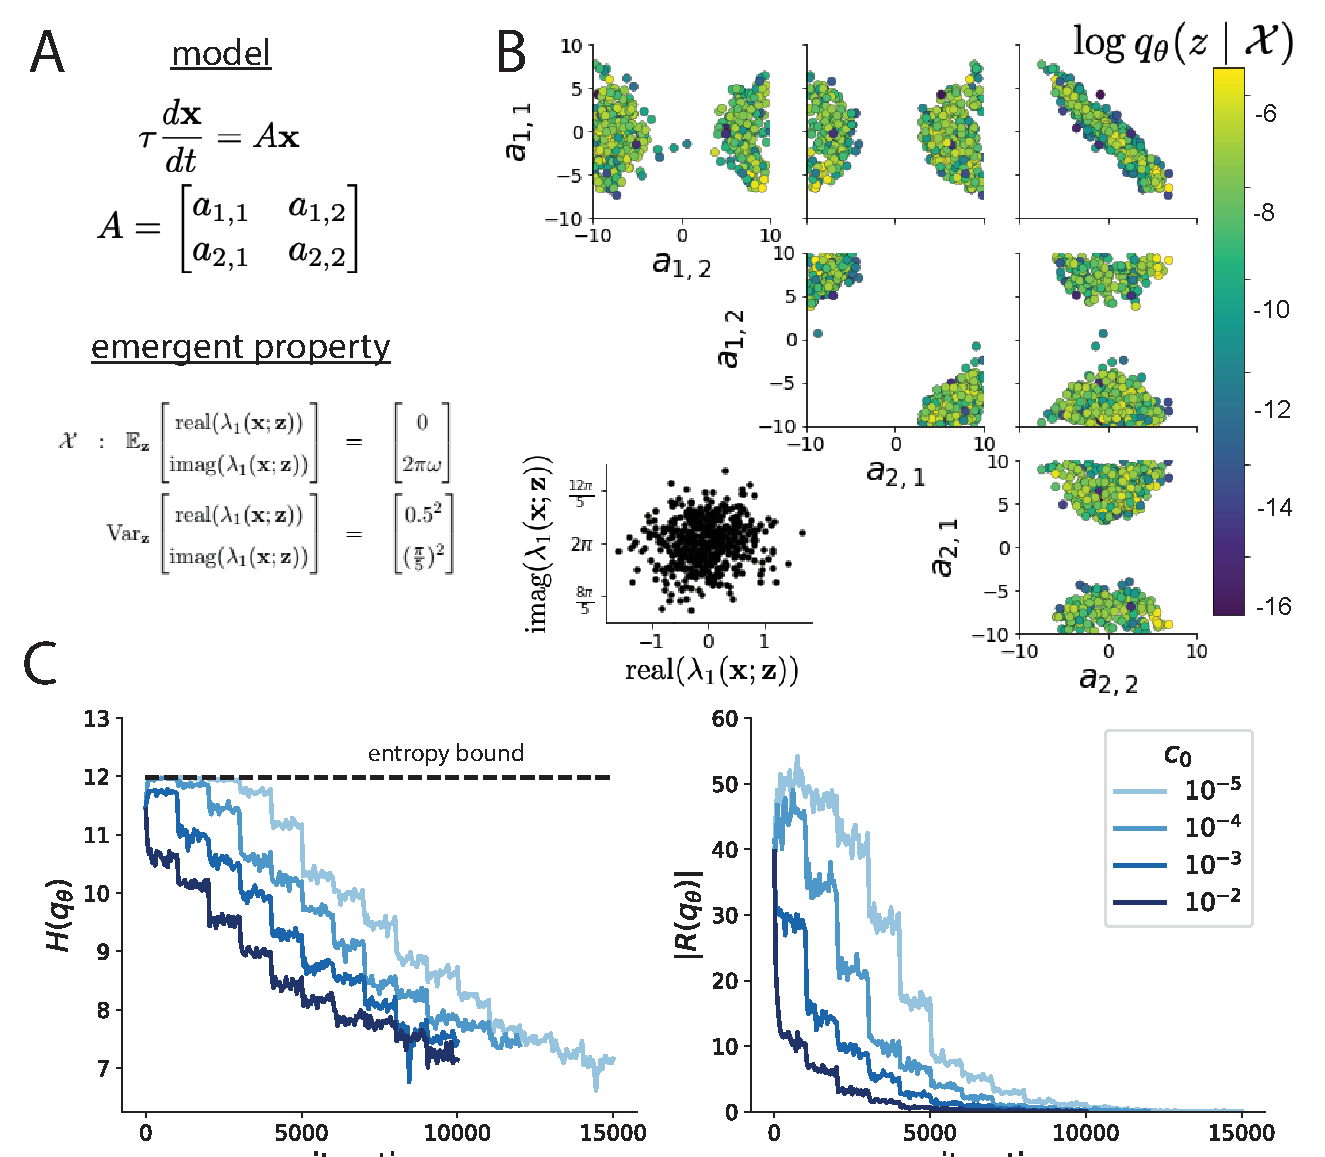
\includegraphics[scale=0.8]{figures/figLDS1/figLDS1.pdf}
\end{center}
\begin{flushleft}
\caption{\small (LDS1): A. Two-dimensional linear dynamical system model, where real entries of the dynamics matrix $A$ are the parameters.  
B. The EPI distribution for a two-dimensional linear dynamical system with $\tau=1$ that produces an average of 1Hz oscillations with some small amount of variance.  Dashed lines indicate the parameter axes. 
C. Entropy throughout the optimization.  
At the beginning of each augmented Lagrangian epoch (2,000 iterations), the entropy dipped due to the shifted optimization manifold where emergent property constraint satisfaction is increasingly weighted.  
D. Emergent property moments throughout optimization.  
At the beginning of each augmented Lagrangian epoch, the emergent property moments adjust closer to their constraints.}
\end{flushleft}
\label{fig:LDS1}
\end{figure}

Unlike the models we presented in the main text, this model admits an analytical form for the mean emergent property statistics given parameter $\mathbf{z}$, since the eigenvalues can be calculated using the quadratic formula: 
\begin{equation}
\lambda = \frac{(\frac{a_1 + a_4}{\tau}) \pm \sqrt{(\frac{a_1+a_4}{\tau})^2 + 4(\frac{a_2 a_3 - a_1 a_4}{\tau})}}{2}.
\end{equation}

Importantly, even though $\mathbb{E}_{\mathbf{x}\sim p(\mathbf{x} \mid \mathbf{z})}\left[T(\mathbf{x})\right]$ is calculable directly via a closed form function and does not require simulation, we cannot derive the distribution $q^*_{\bm{\theta}}$ directly.  
This fact is due to the formally hard problem of the backward mapping: finding the natural parameters $\eta$ from the mean parameters $\bm{\mu}$ of an exponential family distribution \cite{wainwright2008graphical}.  
Instead, we used EPI to approximate this distribution (Fig. S1B). We used a real-NVP normalizing flow architecture with four masks, two neural network layers of 15 units per mask, with batch normalization momentum 0.99, mapped onto a support of $z_i \in \left[-10, 10 \right]$. (see Section \ref{methods_NF}).

Even this relatively simple system has nontrivial (though intuitively sensible) structure in the parameter distribution.  
To validate our method, we analytically derived the contours of the probability density from the emergent property statistics and values.
In the $a_1$-$a_4$ plane, the black line at $\text{real}(\lambda_1) = \frac{a_1 + a_4}{2} = 0$, dotted black line at
the standard deviation $\text{real}(\lambda_1) = \frac{a_1 + a_4}{2} \pm 0.25$, and the dotted gray line at twice the standard deviation
$\text{real}(\lambda_1) = \frac{a_1 + a_4}{2} \pm 0.5$ follow the contour of probability density of the samples (Fig. S2A). 
The distribution precisely reflects the desired statistical constraints and model degeneracy in the sum of $a_1$ and $a_4$.
Intuitively, the parameters equivalent with respect to emergent property statistic $\text{real}(\lambda_1)$ have similar log densities.

\begin{figure}
\begin{center}
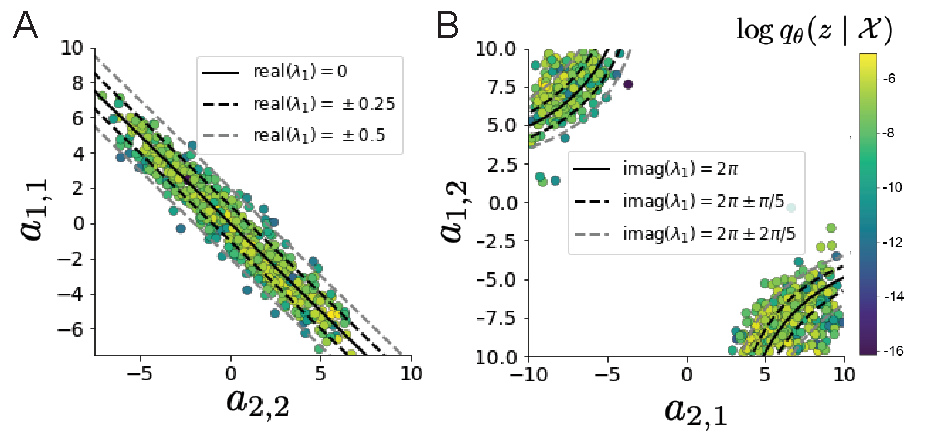
\includegraphics[scale=0.8]{figures/figLDS2/figLDS2.pdf}
\end{center}
\begin{flushleft}
\caption{\small (LDS2): A. Probability contours in the $a_1$-$a_4$ plane were derived from the relationship to emergent property statistic of growth/decay factor $\text{real}(\lambda_1)$. 
B. Probability contours in the $a_2$-$a_3$ plane were derived from the emergent property statistic of oscillation frequency $2\pi \text{imag}(\lambda_1)$.}
\end{flushleft}
\label{fig:LDS2}
\end{figure}

To explain the bimodality of the EPI distribution, we examined the imaginary component of $\lambda_1$.  When $\text{real}(\lambda_1) = \frac{a_1 + a_4}{2} = 0$, we have
\begin{equation}
\text{imag}(\lambda_1) = \begin{cases}
                             \sqrt{\frac{a_1 a_4 - a_2 a_3}{\tau}},  & \text{if } a_1 a_4 < a_2 a_3 \\
                             0 & \text{otherwise } \\
                         \end{cases}.
\end{equation}

When $\tau=1$ and $a_1 a_4 > a_2 a_3$ (center of distribution above), we have the following equation for the other two dimensions:
\begin{equation}
\text{imag}(\lambda_1)^2 = a_1 a_4 - a_2 a_3
\end{equation}
Since we constrained $\mathbb{E}_{\mathbf{z} \sim q_{\bm{\theta}}}\left[\text{imag}(\lambda)\right] = 2 \pi$ (with $\omega=1$), we can plot contours of the equation $\text{imag}(\lambda_1)^2 = a_1 a_4 - a_2 a_3 = (2 \pi)^2$ for various $a_1 a_4$ (Fig. S2B). 
With $\sigma_{1,4} = \mathbb{E}_{\mathbf{z} \sim q_{\bm{\theta}}}(|a_1 a_4 - E_{q_{\bm{\theta}}}[a_1 a_4]|)$, we show the contours as $a_1 a_4 = 0$ (black), $a_1 a_4 = -\sigma_{1,4}$ (black dotted), and $a_1 a_4 = -2\sigma_{1,4}$ (grey dotted). 
This validates the curved structure of the inferred distribution learned through EPI.  
We took steps in negative standard deviation of $a_1 a_4$ (dotted and gray lines), since there are few positive values $a_1 a_4$ in the learned distribution.  
Subtler combinations of model and emergent property will have more complexity, further motivating the use of EPI for understanding these systems.  
As we expect, the distribution results in samples of two-dimensional linear systems oscillating near 1Hz (Fig. S3).

\begin{figure}
\begin{center}
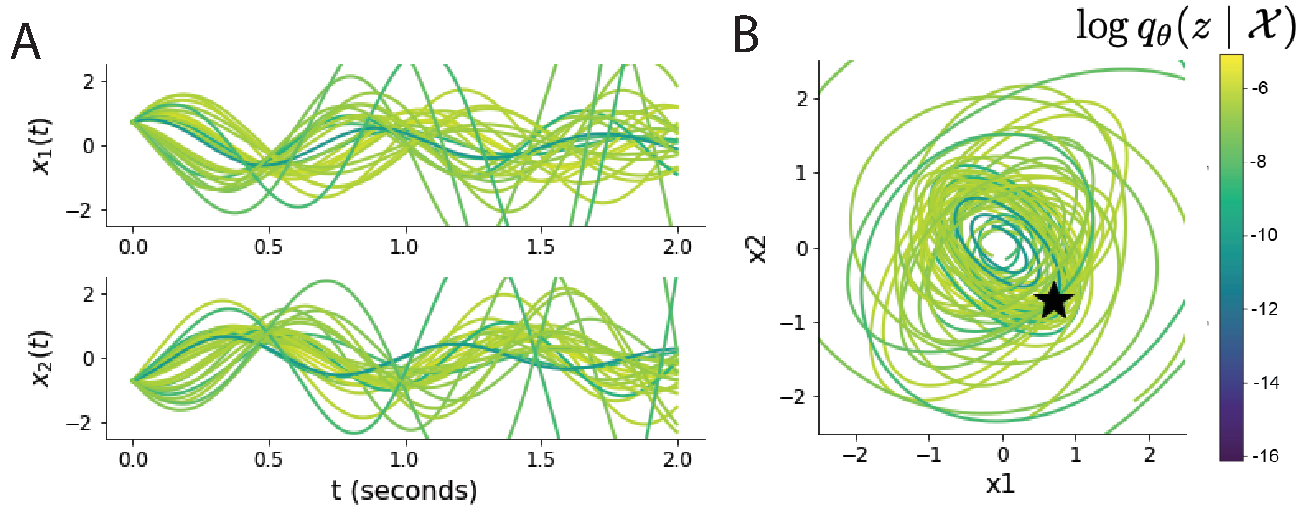
\includegraphics[scale=0.8]{figures/figLDS3/figLDS3.pdf}
\end{center}
\begin{flushleft}
\caption{\small (LDS3): Sampled dynamical systems $\mathbf{z} \sim q_{\bm{\theta}}(\mathbf{z})$ and their simulated activity from $\mathbf{x}(0) = [\frac{\sqrt{2}}{2}, -\frac{\sqrt{2}}{2}]$ colored by log probability. A. Each dimension of the simulated trajectories throughout time.  
B  The simulated trajectories in phase space.}
\end{flushleft}
\label{fig:LDS3}
\end{figure}


\subsubsection{Maximum entropy distributions and exponential families}\label{methods_ME_EF}
%As we compare EPI to variational inference, it is important to consider that EPI is a maximum entropy method, and that maximum entropy methods have a fundamental relationship with exponential family distributions. 
%A maximum entropy distribution of form:
%\begin{equation} \label{eq:max_ent}
%\begin{split}
%p^*(\mathbf{z}) &= \argmax_{p \in \mathcal{P}} H(p(\mathbf{z})) \\
% &  \text{s.t.  } \mathbb{E}_{\mathbf{z} \sim p}\left[T(\mathbf{z})\right] = \bm{\mu}. \\
% \end{split}
%\end{equation} 
%will have probability density in the exponential family:
%\begin{equation}
%p^*(\mathbf{z}) \propto \exp(\bm{\eta}^\top T(\textbf{z})).
%\end{equation}
%The mappings between the mean parameterization $\bm{\mu}$ and the natural parameterization $\bm{\eta}$ are formally hard to identify \cite{wainwright2008graphical}.
Maximum entropy distributions have a fundamental link to exponential family distributions. 
A maximum entropy distribution of form:
\begin{equation} \label{eq:max_ent}
\begin{split}
p^*(\mathbf{z}) &= \argmax_{p \in \mathcal{P}} H(p(\mathbf{z})) \\
 &  \text{s.t.  } \mathbb{E}_{\mathbf{z} \sim p}\left[T(\mathbf{z})\right] = \bm{\mu}_{\text{opt}}. \\
 \end{split}
\end{equation} 
will have probability density in the exponential family:
\begin{equation}
p^*(\mathbf{z}) \propto \exp(\bm{\eta}^\top T(\textbf{z})).
\end{equation}
The mappings between the mean parameterization $\bm{\mu}_{\text{opt}}$ and the natural parameterization $\bm{\eta}$ are formally hard to identify \cite{wainwright2008graphical}.

In EPI, emergent properties are defined as statistics having a fixed mean and variance as in Equation \ref{eq:EP_STG}
 \begin{equation}
\mathbb{E}_{\mathbf{z},\mathbf{x}}\left[f(\mathbf{x}; \mathbf{z})\right] = \bm{\mu}, \text{Var}_{\mathbf{z},\mathbf{x}}\left[f(\mathbf{x}; \mathbf{z})\right] = \bm{\sigma}^2.
\end{equation}
The variance constraint is a second moment constraint on $f(\mathbf{x}; \mathbf{z})$
 \begin{equation}
\text{Var}_{\mathbf{z},\mathbf{x}}\left[f(\mathbf{x}; \mathbf{z})\right] = \mathbb{E}_{\mathbf{z},\mathbf{x}}\left[\left( f(\mathbf{x}; \mathbf{z}) - \bm{\mu}\right) ^2\right]
\end{equation}
As a general maximum entropy distribution (Equation \ref{eq:max_ent}), the sufficient statistics vector contains both first and second order moments of $f(\mathbf{x}; \mathbf{z})$
\begin{equation} \label{eq:moments}
T(\mathbf{x}; \mathbf{z}) = \begin{bmatrix} f(\mathbf{x}; \mathbf{z}) \\ \left( f(\mathbf{x}; \mathbf{z}) - \bm{\mu} \right)^2 \end{bmatrix},
\end{equation}
which are constrained to the chosen means and variances
\begin{equation} \label{eq:mu_opt}
\bm{\mu}_{\text{opt}} = \begin{bmatrix} \bm{\mu} \\ \bm{\sigma}^2 \end{bmatrix}.
\end{equation}


\subsubsection{EPI as variational inference}\label{methods_VI}
%Now that we have fully described the EPI method, we  consider its broader contextualization as a statistical method and its relation to Bayesian inference. 
In Bayesian inference a prior belief about model parameters $\mathbf{z}$ is stated in a prior distribution $p(\mathbf{z})$, and the statistical model capturing the effect of $\mathbf{z}$ on observed data points $\mathbf{x}$ is formalized in the likelihood distribution $p(\mathbf{x} \mid \mathbf{z})$.
In Bayesian inference, we obtain a posterior distribution $p(z \mid \mathbf{x})$, which captures how the data inform our knowledge of model parameters using Bayes' rule:
\begin{equation}
p(\mathbf{z} \mid \mathbf{x}) = \frac{p(\mathbf{x} \mid \mathbf{z}) p(\mathbf{z})}{p(\mathbf{x})}.
\end{equation}
The posterior distribution is analytically available when the prior is conjugate with the likelihood.
However, conjugacy is rare in practice, and alternative methods, such as variational inference \cite{blei2017variational}, are utilized.

%Now, consider the goal of doing variational inference with an exponential family posterior distribution $p(z \mid \mathbf{x})$.  
%We use the following abbreviated notation to collect the base measure $b(z)$ and sufficient statistics $T(z)$ into $\tilde{T}(z)$ and likewise concatenate a 1 onto the end of the natural parameter $\tilde{\eta}(\mathbf{x})$.  
%The log normalizing constant $A(\eta(\mathbf{x}))$ remains unchanged:
%\begin{equation}
%\begin{split}
%p(z \mid \mathbf{x}) = b(z) \exp{\left( \eta(\mathbf{x})^\top T(z) - A(\eta(\mathbf{x})) \right)} = \exp{\left( \begin{bmatrix} \eta(\mathbf{x}) \\ 1 \end{bmatrix}^\top \begin{bmatrix} T(z) \\ b(z) \end{bmatrix} - A(\eta(\mathbf{x})) \right)} \\= \exp{\left(\tilde{\eta(\mathbf{x})}^\top \tilde{T}(z) - A(\eta(\mathbf{x})) \right)} 
%\end{split}.
%\end{equation}
%Variational inference with an exponential family posterior distribution uses optimization to minimize the following divergence \cite{blei2017variational}:
%\begin{equation}
%q_{\bm{\theta}}^* = \argmin_{q_{\bm{\theta}} \in Q} KL(q_{\bm{\theta}} \mid \mid p(z \mid \mathbf{x})).
%\end{equation}
%$q_{\bm{\theta}}(z)$ is the variational approximation to the posterior with variational parameters $\bm{\theta}$.  
%We can write this KL divergence in terms of entropy of the variational approximation:
%\begin{equation}
%KL(q_{\bm{\theta}} \mid \mid p(z \mid \mathbf{x})) = \mathbb{E}_{z \sim q_{\bm{\theta}}} \left[ \log (q_{\bm{\theta}}(z)) \right] - \mathbb{E}_{z \sim q_{\bm{\theta}}} \left[ \log (p(z \mid \mathbf{x})) \right]
%\end{equation}
%\begin{equation}
% = -H(q_{\bm{\theta}}) - \mathbb{E}_{z \sim q_{\bm{\theta}}} \left[ \tilde{\eta}(\mathbf{x})^\top  \tilde{T}(z) - A(\eta(\mathbf{x})) \right].
%\end{equation}
%As far as the variational optimization is concerned, the log normalizing constant is independent of $q_{\bm{\theta}}(z)$, so it can be dropped
%\begin{equation}
%\argmin_{q_{\bm{\theta}} \in Q} KL(q_{\bm{\theta}} \mid \mid p(z \mid \mathbf{x})) =  \argmin_{q_{\bm{\theta}} \in Q} -H(q_{\bm{\theta}}) - \mathbb{E}_{z \sim q_{\bm{\theta}}} \left[ \tilde{\eta}(\mathbf{x})^\top  \tilde{T}(z) \right].
%\end{equation}
% Further, we can write the objective in terms of the first moment of the sufficient statistics $\bm{\mu} = \mathbb{E}_{z \sim p(z \mid \mathbf{x})}\left[T(z) \right]$:
% \begin{equation}
%=  \argmin_{q_{\bm{\theta}} \in Q} -H(q_{\bm{\theta}}) - \mathbb{E}_{z \sim q_{\bm{\theta}}} \left[ \tilde{\eta}(\mathbf{x})^\top \left(  \tilde{T}(z) -\bm{\mu} \right) \right] + \tilde{\eta}(\mathbf{x})^\top \bm{\mu},
% \end{equation}
%which simplifies to
%  \begin{equation}
%=  \argmin_{q_{\bm{\theta}} \in Q} -H(q_{\bm{\theta}}) - \mathbb{E}_{z \sim q_{\bm{\theta}}} \left[ \tilde{\eta}(\mathbf{x})^\top \left(  \tilde{T}(z) -\bm{\mu} \right) \right].
% \end{equation}.
%
%In comparison, in emergent property inference (EPI), we solve the following problem:
%\begin{equation}
%q_{\bm{\theta}}^*(z) = \argmax_{q_{\bm{\theta}} \in Q} H(q_{\bm{\theta}}(z)),   \text{  s.t.  } \mathbb{E}_{z \sim q_{\bm{\theta}}}\left[ \mathbb{E}_{\mathbf{x}\sim p(\mathbf{x} \mid z)}\left[T(\mathbf{x})\right] \right] = \bm{\mu}.
%\end{equation}
%The Lagrangian objective (without augmentation) is
%\begin{equation}
%q_{\bm{\theta}}^* = \argmin_{q_{\bm{\theta}} \in Q} - H(q_{\bm{\theta}}) + \eta_{\text{opt}}^\top \left(\mathbb{E}_{z \sim q_{\bm{\theta}}} \left[\tilde{T}(z) \right] - \bm{\mu} \right).
%\end{equation}
%Thus, as the optimization proceeds, $\eta_{\text{opt}}^\top$ should converge to the natural parameter $\tilde{\eta}(\mathbf{x})$ through its adaptations in each epoch (see Section \ref{methods_AL_opt}). 
%
%We have shown that there is indeed a clear relationship between Bayesian inference and EPI.
%Specifically, EPI is executing variational inference in an exponential family posterior,  whose sufficient statistics are the emergent property statistics and mean parameterization are the emergent property values.
%However, in EPI we  have not specified a prior distribution, or collected data, which can inform us about model parameters.
%Instead we have a mathematical specification of an emergent property, which the model must produce, and a maximum entropy selection principle.
%Accordingly, we replace the notation of $p(\mathbf{z} \mid \mathbf{x})$ with $p(\mathbf{z} \mid \mathcal{B})$ conceptualizing an inferred distribution that obeys emergent property $\mathcal{B}$ (see Section \ref{methods_EPI}). 

In variational inference, a posterior approximation $q_{\bm{\theta}}^*$ is chosen from within some variational family $\mathcal{Q}$
\begin{equation}
q_{\bm{\theta}}^*(\mathbf{z}) = \argmin_{q_{\bm{\theta}} \in Q} KL(q_{\bm{\theta}}(\mathbf{z}) \mid \mid p(\mathbf{z} \mid \mathbf{x})).
\end{equation}
The KL divergence can be written in terms of entropy of the variational approximation:
\begin{equation}
KL(q_{\bm{\theta}}(\mathbf{z})  \mid \mid p(\mathbf{z} \mid \mathbf{x})) = \mathbb{E}_{\mathbf{z} \sim q_{\bm{\theta}}} \left[ \log (q_{\bm{\theta}}(\mathbf{z})) \right] - \mathbb{E}_{\mathbf{z} \sim q_{\bm{\theta}}} \left[ \log (p(\mathbf{z} \mid \mathbf{x})) \right]
\end{equation}
\begin{equation}
= -H(q_{\bm{\theta}}) - \mathbb{E}_{\mathbf{z} \sim q_{\bm{\theta}}} \left[ \log (p(\mathbf{x} \mid \mathbf{z}))  + \log(p(\mathbf{z})) - \log(p(\mathbf{x}))\right]
\end{equation}
Since the marginal distribution of the data $p(\mathbf{x})$ (or ``evidence") is independent of $\bm{\theta}$, variational inference is executed by optimizing the remaining expression.
This is usually framed as maximizing the evidence lower bound (ELBO)
\begin{equation}
\argmin_{q_{\bm{\theta}} \in Q} KL(q_{\bm{\theta}} \mid \mid p(\mathbf{z} \mid \mathbf{x})) = \argmax_{q_{\bm{\theta}} \in Q} H(q_{\bm{\theta}}) + \mathbb{E}_{\mathbf{z} \sim q_{\bm{\theta}}} \left[ \log (p(\mathbf{x} \mid \mathbf{z}))  + \log(p(\mathbf{z}))\right].
\end{equation}

Now, consider the setting where we have chosen a uniform prior, and stipulate a mean-field gaussian likelihood on a chosen statistic of the data $f(\mathbf{x}; \mathbf{z})$
\begin{equation}
p(\mathbf{x} \mid \mathbf{z}) = \mathcal{N}(f(\mathbf{x}; \mathbf{z}) \mid \bm{\mu}_f, \Sigma_f),
\end{equation}
where $\Sigma_f = \text{diag}(\bm{\sigma}_f^2)$.
The log likelihood is then proportional to a dot product of the natural parameter of this mean-field gaussian distribution and the first and second moment statistics.
\begin{equation}
\log p(\mathbf{x} \mid \mathbf{z}) \propto \bm{\eta}_f^\top T(\mathbf{x}, \mathbf{z}),
\end{equation}
where
\begin{equation}
\bm{\eta}_{f} = \begin{bmatrix} \frac{\bm{\mu}_f}{\bm{\sigma}_f^2} \\ \frac{-1}{2\bm{\sigma}_f^2} \end{bmatrix}, \text{ and}
\end{equation}
\begin{equation}
T(\mathbf{x}; \mathbf{z}) = \begin{bmatrix} f(\mathbf{x}; \mathbf{z}) \\ \left( f(\mathbf{x}; \mathbf{z}) - \bm{\mu}_f \right)^2 \end{bmatrix}.
\end{equation}
The variational objective is then
\begin{equation}
\argmax_{q_{\bm{\theta}} \in Q} H(q_{\bm{\theta}}) + \bm{\eta}_f^\top \mathbb{E}_{\mathbf{z} \sim q_{\bm{\theta}}}\left[ T(\mathbf{x}; \mathbf{z}) \right]
\end{equation}

Comparing this to the Lagrangian objective (without augmentation) of EPI, we see they are the same
\begin{equation}
\begin{split}
q_{\bm{\theta}}^*(\mathbf{z}) &= \argmin_{q_{\bm{\theta}} \in Q} - H(q_{\bm{\theta}}) + \bm{\eta}_{\text{opt}}^\top \left(\mathbb{E}_{\mathbf{z}, \mathbf{x}} \left[T(\mathbf{x}; \mathbf{z}) \right] - \bm{\mu}_{\text{opt}} \right) \\
 &= \argmin_{q_{\bm{\theta}} \in Q} - H(q_{\bm{\theta}}) + \bm{\eta}_{\text{opt}}^\top \mathbb{E}_{\mathbf{z}, \mathbf{x}} \left[T(\mathbf{x}; \mathbf{z}) \right].
\end{split}
\end{equation}
where $T(\mathbf{x}; \mathbf{z})$ consists of the first and second moments of the emergent property statistic $f(\mathbf{x}; \mathbf{z})$ (Equation \ref{eq:moments}).
Thus, EPI is implicitly executing variational inference with a uniform prior and a mean-field gaussian likelihood on the emergent property statistics.
The data $\mathbf{x}$ used by this implicit variational inference program would be that generated by the adapting variational approximation $\mathbf{x} \sim p(\mathbf{x} \mid \mathbf{z}) q_{\bm{\theta}}(\mathbf{z})$, and the likelihood parameters $\bm{\eta}_{f}$ of EPI optimization epoch $k$ are predicated by $\bm{\eta}_{\text{opt},k}$ .
However, in EPI we  have not specified a prior distribution, or collected data, which can inform us about model parameters.
Instead we have a mathematical specification of an emergent property, which the model must produce, and a maximum entropy selection principle.
Accordingly, we replace the notation of $p(\mathbf{z} \mid \mathbf{x})$ with $p(\mathbf{z} \mid \mathcal{X})$ conceptualizing an inferred distribution that obeys emergent property $\mathcal{X}$ (see Section \ref{methods_EPI}). 

\subsection{Theoretical models}\label{methods_theoretical_models}
In this study, we used emergent property inference to examine several models relevant to theoretical neuroscience.  
Here, we provide the details of each model  and the related analyses.

\subsubsection{Stomatogastric ganglion}\label{methods_STG}
%We analyze how the parameters $\mathbf{z} = [ g_{\text{el}}, g_{\text{synA}}]$ govern the emergent phenomena of network syncing in a model of the stomatogastric ganglion (STG) \cite{gutierrez2013multiple} shown in Figure \ref{fig:STG}A with activity $\mathbf{x} = \left[ x_{\text{f1}}, x_{\text{f2}}, x_{\text{hub}}, x_{\text{s1}}, x_{\text{s2}} \right]$, using the same hyperparameter choices as Gutierrez et al.
%Each neuron's membrane potential $x_\alpha(t)$ for $\alpha \in \{ \text{f1}, \text{f2}, \text{hub}, \text{s1}, \text{s2} \}$ is the solution of the following differential equation:
%\begin{equation} C_m \frac{dx_\alpha}{dt} = - \left[ h_{leak}(\mathbf{x}; \mathbf{z}) + h_{Ca}(\mathbf{x}; \mathbf{z}) + h_K(\mathbf{x}; \mathbf{z}) + h_{hyp}(\mathbf{x}; \mathbf{z}) + h_{elec}(\mathbf{x}; \mathbf{z}) + h_{syn}(\mathbf{x}; \mathbf{z})\right].
%\end{equation} 
%The membrane potential of each neuron is affected by the leak, calcium, potassium, hyperpolarization, electrical and synaptic currents, respectively, which are functions of  all membrane potentials and the conductance parameters $\mathbf{z}$.  
%The capacitance of the cell membrane was set to $C_m = 1nF$. Specifically, the currents are the difference in the neuron's membrane potential and that current type's reversal potential multiplied by a conductance:
%\begin{equation}  h_{leak}(\mathbf{x}; \mathbf{z}) = g_{leak} (x_\alpha - V_{leak}) 
%\end{equation} 
%\begin{equation}  h_{elec}(\mathbf{x}; \mathbf{z}) = g_{\text{el}} (x_\alpha^{post} - x_\alpha^{pre})
%\end{equation} 
%\begin{equation}  h_{syn}(\mathbf{x}; \mathbf{z}) = g_{syn} S_\infty^{pre} (x_\alpha^{post} - V_{syn}) \end{equation} 
%\begin{equation}  h_{Ca}(\mathbf{x}; \mathbf{z}) = g_{Ca} M_\infty (x_\alpha - V_{Ca}) 
%\end{equation} 
%\begin{equation}  h_K(\mathbf{x}; \mathbf{z}) = g_K N (x_\alpha - V_K) 
%\end{equation} 
%\begin{equation}  h_{hyp}(\mathbf{x}; \mathbf{z}) = g_h H(x_\alpha - V_{hyp}).
%\end{equation} 
%The reversal potentials were set to $V_{leak} = -40mV$, $V_{Ca} = 100mV$, $V_K = -80mV$, $V_{hyp} = -20mV$, and $V_{syn} = -75mV$.  
%The other conductance parameters were fixed to $g_{leak} = 1 \times 10^{-4} \mu S$. $g_{Ca}$, $g_{K}$, and $g_{hyp}$ had different values based on fast, intermediate (hub) or slow neuron.  
%The fast conductances had values $g_{Ca} = 1.9 \times 10^{-2}$, $ g_K = 3.9 \times 10^{-2} $, and $ g_{hyp} = 2.5 \times 10^{-2} $.  
%The intermediate conductances had values $g_{Ca} = 1.7 \times 10^{-2}$, $ g_K = 1.9 \times 10^{-2} $, and $ g_{hyp} = 8.0 \times 10^{-3} $.  
%Finally, the slow conductances had values $g_{Ca} = 8.5 \times 10^{-3}$, $ g_K = 1.5 \times 10^{-2} $, and $ g_{hyp} = 1.0 \times 10^{-2} $.
%
%Furthermore, the Calcium, Potassium, and hyperpolarization channels have time-dependent gating dynamics dependent on steady-state gating variables $M_\infty$, $N_\infty$ and $H_\infty$, respectively:
%\begin{equation}  M_{\infty} = 0.5 \left( 1 + \tanh \left( \frac{x_\alpha - v_1}{v_2} \right) \right) \end{equation}
%\begin{equation}  \frac{dN}{dt} = \lambda_N (N_\infty - N)  \end{equation}
%\begin{equation}  N_\infty = 0.5 \left( 1 + \tanh \left( \frac{x_\alpha - v_3}{v_4} \right) \right) \end{equation}
%\begin{equation}  \lambda_N = \phi_N \cosh \left( \frac{x_\alpha - v_3}{2 v_4} \right) \end{equation}
%\begin{equation}  \frac{dH}{dt} = \frac{\left( H_\infty - H \right)}{\tau_h} \end{equation}
%\begin{equation}  H_\infty = \frac{1}{1 + \exp \left( \frac{x_\alpha + v_5}{v_6} \right)} \end{equation}
%\begin{equation}  \tau_h = 272 - \left( \frac{-1499}{1 + \exp \left( \frac{-x_\alpha + v_7}{v_8} \right)} \right).
% \end{equation}
%where we set $v_1 = 0mV$, $v_2  = 20mV$, $v_3 = 0mV$, $v_4 = 15mV$, $v_5 = 78.3mV$,
%$v_6 = 10.5mV$, $v_7 = -42.2mV$, $v_8 = 87.3mV$, $v_9 = 5mV$, and $v_{th} = -25mV$.  
%
%Finally, there is a synaptic gating variable as well:
%\begin{equation} S_\infty = \frac{1}{1 + \exp \left( \frac{v_{th} - x_\alpha}{v_9} \right)} .
%\end{equation}
%When the dynamic gating variables are considered, this is actually a 15-dimensional nonlinear dynamical system.
%
%In order to measure the frequency of the hub neuron during EPI, the STG model was simulated for $T = 200$ time steps of $dt = 25ms$.  
%In EPI, since gradients are taken through the simulation process, the number of time steps are kept modest if possible. 
%The chosen $dt$ and $T$ were the most computationally convenient choices yielding accurate frequency measurement.  
%Poor resolution afforded by the discrete Fourier transform motivated the use of an alternative basis of complex exponentials to measure spiking frequency.  
%Instead, we used a basis of complex exponentials with frequencies from 0.0-1.0 Hz at 0.01Hz resolution, $\Phi = \left[ 0.0, 0.01, ..., 1.0 \right]^\top$
%
%Another consideration was that the frequency spectra of the neuron membrane potentials had several peaks.  
%High-frequency sub-threshold activity obscured the maximum frequency measurement in the complex exponential basis.  
%Accordingly, subthreshold activity was set to zero, and the whole signal was low-pass filtered with a moving average window of length 20.  
%The signal was subsequently mean centered.  
%After this preprocessing, the maximum frequency in the filter bank accurately reflected the firing frequency.
%
%Finally, to differentiate through the maximum frequency identification, we used a sum-of-powers normalization.  
%Let $\mathcal{X}_\alpha \in \mathcal{C}^{|\Phi|}$ be the complex exponential filter bank dot products with the signal $x_\alpha \in \mathbb{R}^{N}$, where $\alpha \in \{ \text{f1}, \text{f2}, \text{hub}, \text{s1}, \text{s2} \}$.  
%The ``frequency identification" vector is 
%\begin{equation}
%v_\alpha = \frac{|\mathcal{X}_\alpha|^\beta}{\sum_{k=1}^N |\mathcal{X}_\alpha(k)|^\beta}.
%\end{equation}
%The frequency is then calculated as $\omega_\alpha = v_\alpha^\top \Phi$ with $\beta = 100$.
%
%Network syncing, like all other emergent properties in this work, are defined by the emergent property statistics and values.  
%The emergent property statistics are the first and second moments of the firing frequencies. 
%The first moments were set to 0.53Hz, and the second moments were set to 0.025Hz$^2$:
%\begin{equation}
%E \begin{bmatrix} \omega_{\text{f1}} \\ \omega_{\text{f2}} \\ \omega_{\text{hub}} \\ \omega_{\text{s1}} \\ \omega_{\text{s2}} \\ (\omega_{\text{f1}} - 0.53)^2 \\ (\omega_{\text{f2}} - 0.53)^2 \\ (\omega_{\text{hub}} - 0.53)^2 \\ (\omega_{\text{s1}} - 0.53)^2 \\ (\omega_{\text{s2}} - 0.53)^2  \end{bmatrix} = \begin{bmatrix} 0.53 \\ 0.53 \\ 0.53 \\ 0.53 \\ 0.53 \\ 0.025^2 \\ 0.025^2 \\ 0.025^2 \\ 0.025^2 \\ 0.025^2 \end{bmatrix}
%\end{equation}
%for the EPI distribution shown in Fig. \ref{fig:STG}B.
%Throughout optimization, the augmented Lagrangian parameters $\eta$ and $c$, were updated after each epoch of 2,500 iterations (see Section \ref{methods_AL_opt}).  
%The optimization converged after four epochs (Fig. S4).
%
%\begin{figure}
%\begin{center}
%\includegraphics[scale=0.6]{figures/figS4/figS4.pdf}
%\end{center}
%\begin{flushleft}
%{\small Fig. S4: EPI optimization of the STG model producing network syncing. 
%A. Entropy throughout optimization. 
%B. The first moment emergent property statistics converge to the emergent property values at 10,000 iterations, following the fourth augmented Lagrangian epoch of 2,500 iterations.  
%Since $q_{\bm{\theta}}(\mathbf{z})$ failed to produce enough samples yielding $\omega_{\text{f1}}(\mathbf{x})$ less than $0.53$Hz, the convergence criteria were not satisfied after the third epoch at 7,500 iterations.    
%C. The second moment emergent property statistics converge to the emergent property values.}
%\end{flushleft}
%\end{figure}
%
%For EPI in Fig 2C, we used a real NVP architecture with four masks and two layers of 10 units per mask, and batch normalization momentum of 0.99 mapped onto a support of $\mathbf{z} = [g_{\text{el}}, g_{\text{synA}}] \in [4,8] \times [0,4]$. 
%We used an augmented Lagrangian coefficient of $c_0 = 10^{2}$, a batch size $n=300$, set $\nu = 0.1$, and initialized $q_{\bm{\theta}}(\mathbf{z})$ to produce an isotropic 
%Gaussian with mean $\mu_{\text{init}} = [6, 2]$ with standard deviation $\sigma_{\text{init}} = 0.5$.
%
%We calculated the Hessian at the mode of the inferred EPI distribution.  
%The Hessian of a probability model is the second order gradient of the log probability density $\log q_{\bm{\theta}}(\mathbf{z})$ with respect to the parameters $\mathbf{z}$:  $\frac{\partial^2 \log q_{\bm{\theta}}(\mathbf{z})}{\partial \mathbf{z} \partial \mathbf{z}^\top}$.  
%With EPI, we can examine the Hessian, which is analytically available throughout distribution, to indicate the dimensions of parameter space that are sensitive (high magnitude eigenvalue), and which are degenerate (low magnitude eigenvalue) with respect to the emergent property produced. 
%In Figure \ref{fig:STG}B, the eigenvectors of the Hessian $v_1$ and $v_2$ are shown evaluated at the mode of the distribution.  
%The length of the arrows is inversely proportional to the square root of absolute value of their eigenvalues $\lambda_1 = -10.8$ and $\lambda_2 = -2.27$.
%We quantitatively measured the sensitivity of the model with respect to network syncing along the eigenvectors of the Hessian (Fig. \ref{fig:STG}B, inset).
%Sensitivity was measured as the slope coefficient of linear regression fit to network syncing error (the sum of squared differences of each neuron's frequency from 0.53Hz) as a function of parametric perturbation magnitude (maximum 0.25) away from the mode along both orientations indicated by the eigenvector with 100 equally spaced samples.
%The sensitivity slope coefficient of eigenvector $v_1$ with respect to network syncing was significant ($\beta = 4.82 \times 10^{-2}$, $p<10^{-4}$).
%In contrast, eigenvector $v_2$ did not identify a dimension of parameter space significantly sensitive to network syncing ($\beta = 8.65 \times 10^{-4}$ with $p=.67$).
%These sensitivities were compared to all other dimensions of parameter space (100 equally spaced angles from 0 to $\pi$), revealing that the Hessian eigenvectors indeed identified the directions of greatest sensitivity and degeneracy (Fig. \ref{fig:STG}B, inset).
%The contours of Figure \ref{fig:STG} were calculated as error in $T(\mathbf{x})$ from $\mu$ in both the first and second moment emergent property statistics.

We analyze how the parameters $\mathbf{z} = [ g_{\text{el}}, g_{\text{synA}}]$ govern the emergent phenomena of intermediate hub frequency in a model of the stomatogastric ganglion (STG) \cite{gutierrez2013multiple} shown in Figure \ref{fig:STG}A with activity $\mathbf{x} = \left[ x_{\text{f1}}, x_{\text{f2}}, x_{\text{hub}}, x_{\text{s1}}, x_{\text{s2}} \right]$, using the same hyperparameter choices as Gutierrez et al.
Each neuron's membrane potential $x_\alpha(t)$ for $\alpha \in \{ \text{f1}, \text{f2}, \text{hub}, \text{s1}, \text{s2} \}$ is the solution of the following stochastic differential equation:
\begin{equation} C_m \frac{dx_\alpha}{dt} = - \left[ h_{leak}(\mathbf{x}; \mathbf{z}) + h_{Ca}(\mathbf{x}; \mathbf{z}) + h_K(\mathbf{x}; \mathbf{z}) + h_{hyp}(\mathbf{x}; \mathbf{z}) + h_{elec}(\mathbf{x}; \mathbf{z}) + h_{syn}(\mathbf{x}; \mathbf{z})\right] + dB.
\end{equation} 
The input current of each neuron is the sum of the leak, calcium, potassium, hyperpolarization, electrical and synaptic currents as well as gaussian noise $dB$.
Each current component is a function of all membrane potentials and the conductance parameters $\mathbf{z}$.

The capacitance of the cell membrane was set to $C_m = 1nF$. Specifically, the currents are the difference in the neuron's membrane potential and that current type's reversal potential multiplied by a conductance:
\begin{equation}  h_{leak}(\mathbf{x}; \mathbf{z}) = g_{leak} (x_\alpha - V_{leak}) 
\end{equation} 
\begin{equation}  h_{elec}(\mathbf{x}; \mathbf{z}) = g_{\text{el}} (x_\alpha^{post} - x_\alpha^{pre})
\end{equation} 
\begin{equation}  h_{syn}(\mathbf{x}; \mathbf{z}) = g_{syn} S_\infty^{pre} (x_\alpha^{post} - V_{syn}) \end{equation} 
\begin{equation}  h_{Ca}(\mathbf{x}; \mathbf{z}) = g_{Ca} M_\infty (x_\alpha - V_{Ca}) 
\end{equation} 
\begin{equation}  h_K(\mathbf{x}; \mathbf{z}) = g_K N (x_\alpha - V_K) 
\end{equation} 
\begin{equation}  h_{hyp}(\mathbf{x}; \mathbf{z}) = g_h H(x_\alpha - V_{hyp}).
\end{equation} 
The reversal potentials were set to $V_{leak} = -40mV$, $V_{Ca} = 100mV$, $V_K = -80mV$, $V_{hyp} = -20mV$, and $V_{syn} = -75mV$.  
The other conductance parameters were fixed to $g_{leak} = 1 \times 10^{-4} \mu S$. $g_{Ca}$, $g_{K}$, and $g_{hyp}$ had different values based on fast, intermediate (hub) or slow neuron.  
The fast conductances had values $g_{Ca} = 1.9 \times 10^{-2}$, $ g_K = 3.9 \times 10^{-2} $, and $ g_{hyp} = 2.5 \times 10^{-2} $.  
The intermediate conductances had values $g_{Ca} = 1.7 \times 10^{-2}$, $ g_K = 1.9 \times 10^{-2} $, and $ g_{hyp} = 8.0 \times 10^{-3} $.  
Finally, the slow conductances had values $g_{Ca} = 8.5 \times 10^{-3}$, $ g_K = 1.5 \times 10^{-2} $, and $ g_{hyp} = 1.0 \times 10^{-2} $.

Furthermore, the Calcium, Potassium, and hyperpolarization channels have time-dependent gating dynamics dependent on steady-state gating variables $M_\infty$, $N_\infty$ and $H_\infty$, respectively:
\begin{equation}  M_{\infty} = 0.5 \left( 1 + \tanh \left( \frac{x_\alpha - v_1}{v_2} \right) \right) \end{equation}
\begin{equation}  \frac{dN}{dt} = \lambda_N (N_\infty - N)  \end{equation}
\begin{equation}  N_\infty = 0.5 \left( 1 + \tanh \left( \frac{x_\alpha - v_3}{v_4} \right) \right) \end{equation}
\begin{equation}  \lambda_N = \phi_N \cosh \left( \frac{x_\alpha - v_3}{2 v_4} \right) \end{equation}
\begin{equation}  \frac{dH}{dt} = \frac{\left( H_\infty - H \right)}{\tau_h} \end{equation}
\begin{equation}  H_\infty = \frac{1}{1 + \exp \left( \frac{x_\alpha + v_5}{v_6} \right)} \end{equation}
\begin{equation}  \tau_h = 272 - \left( \frac{-1499}{1 + \exp \left( \frac{-x_\alpha + v_7}{v_8} \right)} \right).
 \end{equation}
where we set $v_1 = 0mV$, $v_2  = 20mV$, $v_3 = 0mV$, $v_4 = 15mV$, $v_5 = 78.3mV$,
$v_6 = 10.5mV$, $v_7 = -42.2mV$, $v_8 = 87.3mV$, $v_9 = 5mV$, and $v_{th} = -25mV$.  

Finally, there is a synaptic gating variable as well:
\begin{equation} S_\infty = \frac{1}{1 + \exp \left( \frac{v_{th} - x_\alpha}{v_9} \right)} .
\end{equation}
When the dynamic gating variables are considered, this is actually a 15-dimensional nonlinear dynamical system.  Gaussian noise $d\mathbf{B}$ of variance $(1 \times 10^{-12})^2$ A$^2$ makes the model stochastic, and introduces variability in frequency at each parameterization $\mathbf{z}$.

In order to measure the frequency of the hub neuron during EPI, the STG model was simulated for $T = 300$ time steps of $dt = 25\text{ms}$.  
The chosen $dt$ and $T$ were the most computationally convenient choices yielding accurate frequency measurement.  
We used a basis of complex exponentials with frequencies from 0.0-1.0 Hz at 0.01Hz resolution to measure frequency from simulated time series
\begin{equation}
\Phi = \left[ 0.0, 0.01, ..., 1.0 \right]^\top..
\end{equation}

To measure spiking frequency, we processed simulated membrane potentials with a relu (spike extraction) and low-pass filter with averaging window of size 20, then took the frequency with the maximum absolute value of the complex exponential basis coefficients of the processed time-series.  The first 20 temporal samples of the simulation are ignored to account for initial transients.

To differentiate through the maximum frequency identification, we used a soft-argmax
Let $X_\alpha \in \mathcal{C}^{|\Phi|}$ be the complex exponential filter bank dot products with the signal $x_\alpha \in \mathbb{R}^{N}$, where $\alpha \in \{ \text{f1}, \text{f2}, \text{hub}, \text{s1}, \text{s2} \}$.  
The soft-argmax is then calculated using temperature parameter $\beta=100$
\begin{equation}
\psi_\alpha = \text{softmax}(\beta|X_\alpha|\odot i),
\end{equation}
where $i = [0, 1, ..., 100]$.
The frequency is then calculated as 
\begin{equation}
\omega_\alpha = 0.01\psi_\alpha \text{Hz}.
\end{equation}

Intermediate hub frequency, like all other emergent properties in this work, is defined by the mean and variance of the emergent property statistics.
In this case, we have one statistic, hub neuron frequency, where the mean was chosen to be 0.55Hz, and variance was chosen to be (0.025Hz)$^2$ to capture variation in frequency between 0.5Hz and 0.6Hz (Equation \ref{eq:EP_STG}).
As a maximum entropy distribution, $T(\mathbf{x}, \mathbf{z})$ is comprised of both these first and second moments of the hub neuron frequency (as in Equations \ref{eq:moments} and \ref{eq:mu_opt})
\begin{equation} 
T(\mathbf{x}; \mathbf{z}) = \begin{bmatrix} \omega_{\text{hub}}(\mathbf{x}; \mathbf{z}) \\ \left( \omega_{\text{hub}}(\mathbf{x}; \mathbf{z}) - 0.55 \right)^2 \end{bmatrix},
\end{equation}
\begin{equation} 
\bm{\mu}_{\text{opt}} = \begin{bmatrix} 0.55 \\ 0.025^2 \end{bmatrix}.
\end{equation}
Throughout optimization, the augmented Lagrangian parameters $\eta$ and $c$, were updated after each epoch of 5,000 iterations(see Section \ref{methods_AL_opt}).  
The optimization converged after five epochs (Fig. S4).

\begin{figure}
\begin{center}
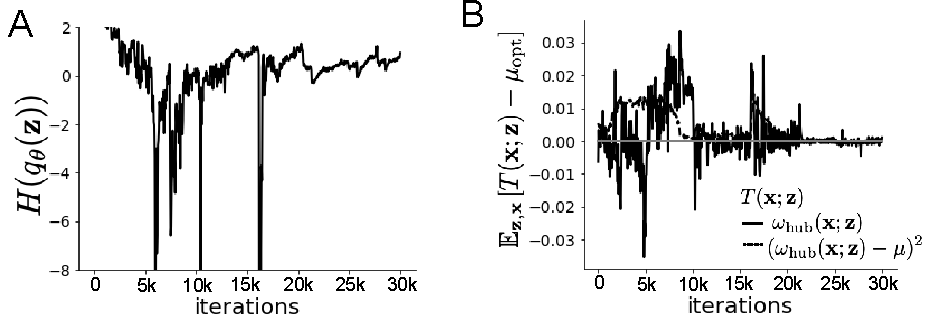
\includegraphics[scale=0.8]{figures/figSTG1/figSTG1.pdf}
\end{center}
\begin{flushleft}
\caption{\small (STG1): EPI optimization of the STG model producing network syncing. 
A. Entropy throughout optimization. 
B. The emergent property statistic means and variances converge to their constraints at 25,000 iterations following the fifth augmented Lagrangian epoch.}
\end{flushleft}
\label{fig:STG1}
\end{figure}

For EPI in Fig \ref{fig:STG}E, we used a real NVP architecture with three Real NVP coupling layers and two-layer neural networks of 25 units per layer.
The normalizing flow architecture mapped $z_0 \sim \mathcal{N}(\mathbf{0}, I)$ to a support of $\mathbf{z} = [g_{\text{el}}, g_{\text{synA}}] \in [4,8] \times [0.01,4]$, initialized to a gaussian approximation of samples returned by a preliminary ABC search.
We did not include $g_{\text{synA}} < 0.01$, for numerical stability.
EPI optimization was run using 5 different random seeds for architecture initialization $\bm{\theta}$ with an augmented Lagrangian coefficient of $c_0 = 10^{5}$, a batch size $n=400$, and $\beta = 2$.
The distribution shown is that of the architecture converging with criteria $N_{\text{test}} = 100$ at greatest entropy across random seeds.

We calculated the Hessian at the mode of the inferred EPI distribution.  
The Hessian of a probability model is the second order gradient of the log probability density $\log q_{\bm{\theta}}(\mathbf{z})$ with respect to the parameters $\mathbf{z}$:  $\frac{\partial^2 \log q_{\bm{\theta}}(\mathbf{z})}{\partial \mathbf{z} \partial \mathbf{z}^\top}$.  
With EPI, we can examine the Hessian, which is analytically available throughout distribution, to indicate the dimensions of parameter space that are sensitive (strongly negative eigenvalue), and which are degenerate (low magnitude eigenvalue) with respect to the emergent property produced. 
In Figure \ref{fig:STG}D, the eigenvectors of the Hessian $v_1$ (solid) and $v_2$ (dashed) are shown evaluated at the mode of the distribution.  
The length of the arrows is inversely proportional to the square root of absolute value of their eigenvalues $\lambda_1 = -10.7$ and $\lambda_2 = -3.22$.
Since the Hessian eigenvectors have sign degeneracy, the visualized directions in 2-D parameter space are chosen arbitrarily.
%We quantitatively measured the sensitivity of the model with respect to network syncing along the eigenvectors of the Hessian (Fig. \ref{fig:STG}B, inset).
%Sensitivity was measured as the slope coefficient of linear regression fit to network syncing error (the sum of squared differences of each neuron's frequency from 0.53Hz) as a function of parametric perturbation magnitude (maximum 0.25) away from the mode along both orientations indicated by the eigenvector with 100 equally spaced samples.
%The sensitivity slope coefficient of eigenvector $v_1$ with respect to network syncing was significant ($\beta = 4.82 \times 10^{-2}$, $p<10^{-4}$).
%In contrast, eigenvector $v_2$ did not identify a dimension of parameter space significantly sensitive to network syncing ($\beta = 8.65 \times 10^{-4}$ with $p=.67$).
%These sensitivities were compared to all other dimensions of parameter space (100 equally spaced angles from 0 to $\pi$), revealing that the Hessian eigenvectors indeed identified the directions of greatest sensitivity and degeneracy (Fig. \ref{fig:STG}B, inset).
%The contours of Figure \ref{fig:STG} were calculated as error in $T(\mathbf{x})$ from $\mu$ in both the first and second moment emergent property statistics.


\subsubsection{Primary visual cortex}\label{methods_V1}
In the stochastic stabilized supralinear network, population rate responses $\mathbf{x}$ to input $\mathbf{h}$, recurrent input $W\mathbf{x}$ and slow noise $\bm{\epsilon}$ are governed by
\begin{equation}
    \tau \frac{d\mathbf{x}}{dt} = -\mathbf{x} +\phi(W\mathbf{x} + \mathbf{h} + \bm{\epsilon}),
\end{equation}
where the noise is an Ornstein-Uhlenbeck process
\begin{equation}
\tau_{\text{noise}} d\epsilon_\alpha = -\epsilon_\alpha dt + \sqrt{2\tau_{\text{noise}}}\sigma_\alpha dB
\end{equation}
with $\tau_{\text{noise}} = 5\text{ms} > \tau = 1\text{ms}$.
As contrast increases, input to the E- and P-populations increases  relative to a baseline input $\mathbf{h} = \mathbf{h}_b + c\mathbf{h}_c$.
Connectivity ($W_{\text{fit}}$) and input ($\mathbf{h}_{b,\text{fit}}$ and $\mathbf{h}_{c,\text{fit}}$) parameters were fit using the deterministic V1 circuit model \cite{palmigiano2020structure} 

\begin{figure}
\begin{center}
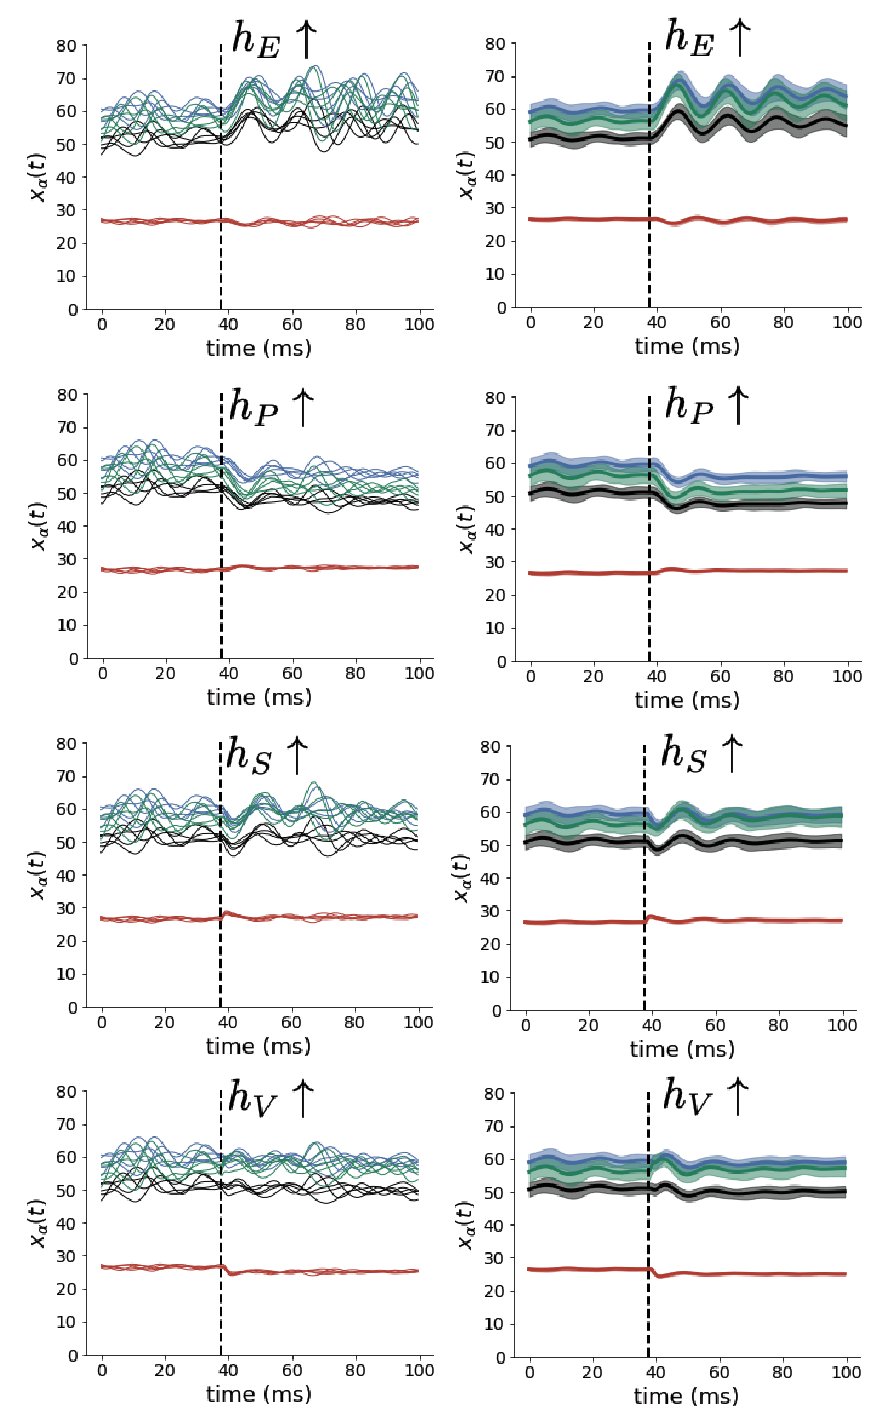
\includegraphics[scale=.8]{figures/figV1_1/figV1_1.pdf}
\end{center}
\caption{\small (V1 1)
(Left) Simulations for small increases in neuron-type population input.
Input magnitudes are chosen so that effect is salient ($0.002$ for E and P, but $0.02$ for S and V).
(Right) Average (solid) and standard deviation (shaded) of stochastic fluctuations of responses.
 }
 \label{fig:V1_1}
\end{figure}

\begin{figure}
\caption{\small (V1 2)
Posterior predictive distributions of the sum of squares of each pair of noise parameters.
 }
 \label{fig:V1_2}
\begin{center}
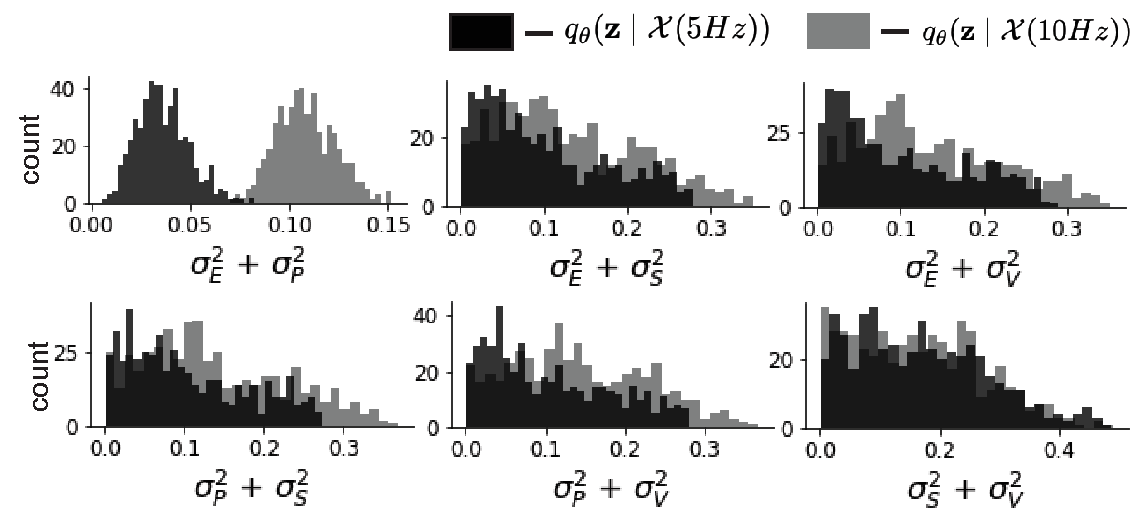
\includegraphics[scale=.8]{figures/figV1_2/figV1_2.pdf}
\end{center}
\end{figure}

\begin{equation}
W_{\text{fit}} =  \begin{bmatrix} W_{EE} & W_{EP} & W_{ES} & W_{EV} \\
W_{PE} & W_{PP} & W_{PS} & W_{PV} \\
W_{SE} & W_{SP} & W_{SS} & W_{SV} \\
W_{VE} & W_{VP} & W_{VS} & W_{VV}  \end{bmatrix} = 
 \begin{bmatrix} 2.18 & -1.19 & -.594 & -.229 \\
 1.66 & -.651 & -.680 & -.242 \\
 .895 & -5.22 \times 10^{-3} & -1.51 \times 10^{-4}   & -.761 \\
 3.34 &  -2.31 & -.254  & -2.52 \times 10^{-4} \\
 \end{bmatrix},
\end{equation} 

\begin{equation}
\mathbf{h}_{b,\text{fit}} =
 \begin{bmatrix} .416 \\ .429 \\ .491 \\ .486 \end{bmatrix} ,
\end{equation} 
and
\begin{equation} 
\mathbf{h}_{c,\text{fit}} = 
\begin{bmatrix} .359 \\ .403 \\ 0 \\ 0 \end{bmatrix}.
\end{equation} 

To obtain rates on a realistic scale (100-fold greater), we map these fitted parameters to an equivalence class

\begin{figure}[h]
\caption{\small (V1 3)
EPI posterior for $\mathcal{X}(10\text{ Hz})$.
 }
 \label{fig:V1_3}
\begin{center}
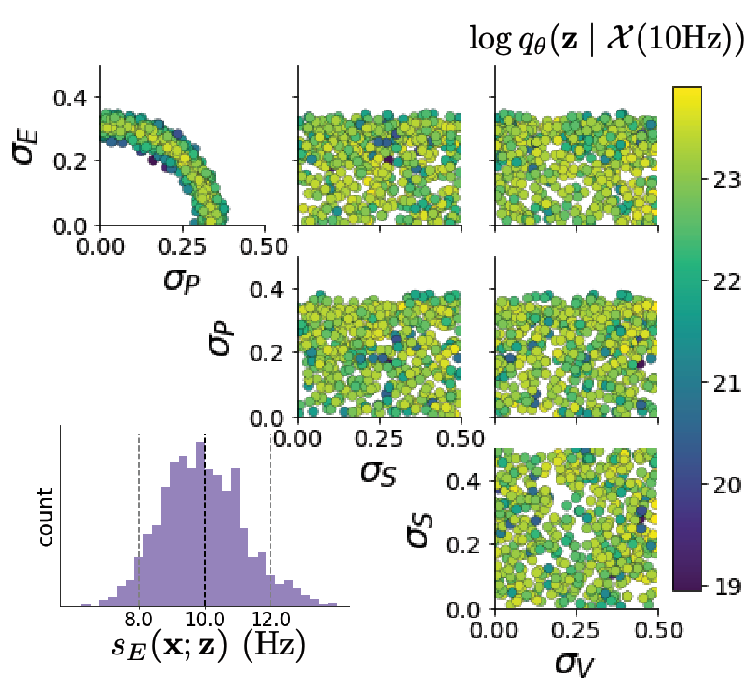
\includegraphics[scale=.8]{figures/figV1_3/figV1_3.pdf}
\end{center}
\end{figure}

\begin{equation}
W =  \begin{bmatrix} W_{EE} & W_{EP} & W_{ES} & W_{EV} \\
W_{PE} & W_{PP} & W_{PS} & W_{PV} \\
W_{SE} & W_{SP} & W_{SS} & W_{SV} \\
W_{VE} & W_{VP} & W_{VS} & W_{VV}  \end{bmatrix} = 
 \begin{bmatrix} .218 & -.119 & -.0594 & -.0229 \\
 .166 & -.0651 & -.068 & -.0242 \\
 .0895 & -5.22 \times 10^{-4} & -1.51 \times 10^{-5}   & -.0761 \\
 .334 &  -.231 & -.0254  & -2.52 \times 10^{-5} \\
 \end{bmatrix},
\end{equation} 

\begin{equation}
\mathbf{h}_b =  \begin{bmatrix} h_{b,E} \\ h_{b,P} \\ h_{b,S} \\ h_{b,V} \end{bmatrix} =
 \begin{bmatrix} 4.16 \\ 4.29 \\ 4.91 \\ 4.86 \end{bmatrix} ,
\end{equation} 
and
\begin{equation} 
\mathbf{h}_c = \begin{bmatrix} h_{c,E} \\ h_{c,P} \\ h_{c,S} \\ h_{c,V} \end{bmatrix} = 
\begin{bmatrix} 3.59 \\ 4.03 \\ 0 \\ 0 \end{bmatrix}.
\end{equation} 

Circuit responses are simulated using $T = 200$ time steps at $dt = 0.5\text{ms}$ from an initial condition drawn from $\mathbf{x}(0) \sim U\left[10\text{ Hz}, 25\text{ Hz}\right]$.
Standard deviation of the E-population $s_E(\mathbf{x}; \mathbf{z})$ is calculated as the square root of the temporal variance from $t_{ss} = 75\text{ms}$ to $Tdt = 100\text{ms}$ averaged over 100 independent trials.
\begin{equation}
s_E(\mathbf{x}; \mathbf{z}) =\mathbb{E}_{x}\left[\sqrt{\mathbb{E}_{t > t_{ss}}\left[\left(x_E(t) -\mathbb{E}_{t > t_{ss}}\left[ x_E(t) \right]\right)^2 \right]}\right]
\end{equation}

For EPI in Fig \ref{fig:V1}D-E, we used a real NVP architecture with three Real NVP coupling layers and two-layer neural networks of 50 units per layer.
The normalizing flow architecture mapped $z_0 \sim \mathcal{N}(\mathbf{0}, I)$ to a support of $\mathbf{z} = [g_{\text{el}}, g_{\text{synA}}] \in [4,8] \times [0.0, 0.5]$.
EPI optimization was run using 3 different random seeds for architecture initialization $\bm{\theta}$ with an augmented Lagrangian coefficient of $c_0 = 10^{-1}$, a batch size $n=100$, and $\beta = 2$.
The distributions shown are those of the architectures converging with criteria $N_{\text{test}} = 100$ at greatest entropy across random seeds.

In Fig. \ref{fig:V1}E, we visualize the modes of $q_{\bm{\theta}}(\mathbf{z} \mid \mathcal{X})$ throughout the $\sigma_E$-$\sigma_P$ marginal.
Specifically, we calculated
\begin{equation}
\begin{split}
\mathbf{z}^*(\sigma_{P,\text{fixed}}) = &\argmax_{\mathbf{z}} \log q_{\bm{\theta}}(\mathbf{z} \mid \mathcal{X}) \\
&\text{s.t. } \sigma_P = \sigma_{P,\text{fixed}}\
\end{split}
\end{equation}
At each mode $\mathbf{z}^*$, we calculated the Hessian and visualized the sensitivity dimension in the direction of positive $\sigma_E$.



\subsubsection{Primary visual cortex: challenges to analysis}\label{methods_V1_complexity}
TODO Agostina and I are putting this together now.

\subsubsection{Superior colliculus}\label{methods_SC}
%In the model of Duan et al \cite{duan2018collicular}, there are four total units: two in each hemisphere corresponding to the Pro/Contra and Anti/Ipsi populations.  
%They are denoted as left Pro (LP), left Anti (LA), right Pro (RP) and right Anti (RA).  
%Each unit has an activity ($x_\alpha$) and internal variable ($u_\alpha$) related by
%\begin{equation}
%x_\alpha =\left(\frac{1}{2}\tanh\left(\frac{u_\alpha - \epsilon}{\zeta}\right)+ \frac{1}{2} \right)
%\end{equation}
%where $\alpha \in \{LP, LA, RA, RP\}$ $\epsilon = 0.05$ and $\zeta = 0.5$ control the position and shape of the nonlinearity, respectively.
%
%We order the elements of $x$ and $u$ in the following manner
%\begin{equation}
%x = \begin{bmatrix} x_{LP} \\ x_{LA} \\ x_{RP} \\ x_{RA} \end{bmatrix} \hspace{2cm} u = \begin{bmatrix} u_{LP} \\ u_{LA} \\ u_{RP} \\ u_{RA} \end{bmatrix}.
%\end{equation}
%
% The internal variables follow dynamics:
%\begin{equation}
%\tau \frac{du}{dt} = -u + Wx + h + \sigma dB
%\end{equation}
%with time constant $\tau = 0.09s$ and Gaussian noise $\sigma dB$ controlled by the magnitude of $\sigma=1.0$.  The weight matrix has 8 parameters $sW_P$, $sW_A$, $vW_{PA}$, $vW_{AP}$, $hW_P$, $hW_A$, $dW_{PA}$, and $dW_{AP}$ (Fig. 4B):
%\begin{equation}
%W = \begin{bmatrix} sW_P & vW_{PA} & hW_P & dW_{PA}  \\ vW_{AP}  & sW_A & dW_{AP}  & hW_A \\ hW_P & dW_{PA}  & sW_P & vW_{PA}  \\ dW_{AP}  & hW_A & vW_{AP}  & sW_A \end{bmatrix}.
%\end{equation}
%
%The system receives five inputs throughout each trial, which has a total length of 1.8s.
%\begin{equation}
%h = h_{\text{rule}} + h_{\text{choice-period}} + h_{\text{light}}.
%\end{equation}
%
%There are rule-based inputs depending on the condition,
%\begin{equation}h_{\text{P,rule}}(t) = \begin{cases}
%                           I_{\text{P,rule}} [1, 0, 1, 0]^\top,& \text{if } t\leq 1.2s \\
%                            0,              & \text{otherwise}
%                         \end{cases}
%\end{equation}
%\begin{equation} h_{\text{A,rule}}(t) = \begin{cases}
%                           I_{\text{A,rule}} [0, 1, 0, 1]^\top,& \text{if } t\leq 1.2s \\
%                            0,              & \text{otherwise}
%                         \end{cases}
%\end{equation}
%a choice-period input,
%\begin{equation} h_{\text{choice}}(t) = \begin{cases}
%                           I_{\text{choice}} [1, 1, 1, 1]^\top,& \text{if } t > 1.2s \\
%                            0,              & \text{otherwise}
%                         \end{cases}
%\end{equation}
%and an input to the right or left-side depending on where the light stimulus is delivered.     
%\begin{equation}  h_{\text{light}}(t) = \begin{cases}
%                           I_{\text{light}} [1, 1, 0, 0]^\top,& \text{if } t > 1.2s \text{ and Left} \\
%                           I_{\text{light}} [0, 0, 1, 1]^\top,& \text{if } t > 1.2s \text{ and Right} \\
%                            0,              & t \leq 1.2s
%                         \end{cases} .
%\end{equation}
%The input parameterization was fixed to $I_{\text{P,rule}} = 10 $,  $I_{\text{A,rule}} = 10$,  $I_{\text{choice}} = 2$,  and $I_{\text{light}} = 1$.
%
%To produce an accuracy rate of $p_{LP}$ in the Left, Pro condition, let $\hat{p}_i$ be the empirical average steady state response (final $x_{LP}$ at end of task) over M=500 Gaussian noise draws for a given SC model parameterization $z_i$:
%\begin{equation}
% \hat{p}_i = \mathbb{E}_{\sigma dB} \left[ x_{LP} \mid s=L, c=P, z=z_i \right] = \frac{1}{M}\sum_{j=1}^M x_{LP}(s=L, c=P, z=z_i, \sigma dB_j)
% \end{equation}
% where stimulus $s \in \{L, R\}$, cue $c \in \{P, A\}$, and $\sigma dB_j$ is the Gaussian noise on trial $j$.
%As with the V1 model, we only consider steady state responses of $x$, so $x_\alpha$ is used from here on to denote the steady state activity at the end of the trial.
%For the first emergent property statistic, the average over EPI samples (from $q_{\bm{\theta}}(z)$) is set to the desired value $p_{LP}$:
%\begin{equation}
%\mathbb{E}_{z_i \sim q_\phi} \left[ \mathbb{E}_{\sigma dB} \left[ x_{LP,\text{ss}} \mid s=L, c=P, z=z_i \right] \right] = \mathbb{E}_{z_i \sim q_\phi} \left[ \hat{p}_i \right] = p_{LP}.
%\end{equation}
%
%For the next emergent property statistic, we ask that the variance of the steady state responses across Gaussian draws, is the Bernoulli variance for the empirical rate $\hat{p}_i$:
%\begin{equation}
%\mathbb{E}_{z \sim q\phi} \left[ \sigma^2_{err} \right] = 0
%\end{equation}
%where the Bernoulli variance error $\sigma^2_{err}$ for the Pro task, left condition is
%\begin{equation}
%\sigma^2_{err} = Var_{\sigma dB} \left[ x_{LP} \mid s=L, c=P, z=z_i \right] - \hat{p}_i(1 - \hat{p}_i).
%\end{equation}
%
%We have an additional constraint that the Pro neuron on the opposite hemisphere should have the opposite value (0 and 1).  We can enforce this with another constraint:
%\begin{equation}
%\mathbb{E}_{z \sim q\phi} \left[ d_P \right] = 1,
%\end{equation}
%where the distance between Pro neuron steady states $d_P$ in the Pro condition is
%\begin{equation}
%d_P =  \mathbb{E}_{\sigma dB} \left[ (x_{LP} - x_{RP})^2  \mid s=L, c=P, z=z_i \right]
%\end{equation}
%The emergent property statistics only need to be measured during the Left stimulus condition of the Pro and Anti tasks, since the network is symmetrically parameterized.
%In total, the emergent property of rapid task switching at accuracy level $p$ was defined as
%\begin{equation}
%\mathcal{B}(p) ~~\triangleq~~ \mathbb{E}\begin{bmatrix} \hat{p}_P \\ \hat{p}_A \\ (\hat{p}_P-p)^2 \\ (\hat{p}_A - p)^2 \\ \sigma^2_{P,err} \\ \sigma^2_{A,err} \\ d_P \\ d_A \end{bmatrix} = \begin{bmatrix} p \\ p \\ 0.15^2 \\ 0.15^2 \\ 0 \\ 0 \\ 1 \\ 1 \end{bmatrix}.
%\end{equation}
%
%Since the maximum variance of a random variable bounded from 0 to 1 is the Bernoulli variance $\hat{p}(1-\hat{p})$, and the maximum squared difference between to variables bounded from 0 to 1 is 1, we do not need to control the second moment of these test statistics. 
%These variables are dynamical system states and can only exponentially decay (or saturate) to 0 (or 1), so the Bernoulli variance error and squared difference constraints cannot be satisfied exactly in simulation.  
%This is important to be mindful of when evaluating the convergence criteria.  
%Instead of using our usual hypothesis testing criteria for convergence to the emergent property, we set a slack variable threshold only for these technically infeasible emergent property values to 0.05.
%
%Using EPI to learn distributions of dynamical systems producing Bernoulli responses at a given rate (with small variance around that rate) was more challenging than expected.  
%There is a pathology in this optimization setup, where the learned distribution of weights is bimodal attributing a fraction $p$ of the samples to an expansive mode (which always sends $x_{LP}$ to 1), and a fraction $1-p$ to a decaying mode (which always sends $x_{LP}$ to 0).  
%This pathology was avoided using an inequality constraint prohibiting parameter samples that resulted in low variance of responses across noise.
%
%
%\begin{table}[h]
%\begin{tabular}{l|l|l|l|l}
%$\lambda$  & $\hat{p}$ & $q_{\bm{\theta}}(z)$ & $r$ & p-value \\ \hline
%$\lambda_{\text{task}}$ & $\hat{p}_P$ & $q(z \mid \mathcal{B}(60\%))$ & $1.24 \times 10^{-01}$ & $p<10^{-4}$  \\ \hline
%$\lambda_{\text{task}}$ & $\hat{p}_P$ & $q(z \mid \mathcal{B}(70\%))$ & $7.56 \times 10^{-01}$ & $p<10^{-4}$ \\ \hline
%$\lambda_{\text{task}}$ & $\hat{p}_P$ & $q(z \mid \mathcal{B}(80\%))$ & $4.59 \times 10^{-01}$ & $p<10^{-4}$  \\ \hline
%$\lambda_{\text{task}}$ & $\hat{p}_P$ & $q(z \mid \mathcal{B}(90\%))$ & $3.76 \times 10^{-01}$ & $p<10^{-4}$  \\ \hline
%
%$\lambda_{\text{task}}$ & $\hat{p}_A$ & $q(z \mid \mathcal{B}(60\%))$ & $4.80 \times 10^{-02}$ & $p<.01$ \\ \hline
%$\lambda_{\text{task}}$ & $\hat{p}_A$ & $q(z \mid \mathcal{B}(70\%))$ & $2.08 \times 10^{-01}$ & $p<10^{-4}$  \\ \hline
%$\lambda_{\text{task}}$ & $\hat{p}_A$ & $q(z \mid \mathcal{B}(80\%))$ & $4.84 \times 10^{-01}$ & $p<10^{-4}$  \\ \hline
%$\lambda_{\text{task}}$ & $\hat{p}_A$ & $q(z \mid \mathcal{B}(90\%))$ & $4.25 \times 10^{-01}$ & $p<10^{-4}$  \\ \hline
%
%$\lambda_{\text{side}}$ & $\hat{p}_P$ & $q(z \mid \mathcal{B}(50\%))$ & $-7.57 \times 10^{-02}$ & $p<10^{-4}$  \\ \hline
%$\lambda_{\text{side}}$ & $\hat{p}_P$ & $q(z \mid \mathcal{B}(60\%))$ & $-6.73 \times 10^{-02}$ & $p<10^{-4}$  \\ \hline
%$\lambda_{\text{side}}$ & $\hat{p}_P$ & $q(z \mid \mathcal{B}(70\%))$ & $-4.86 \times 10^{-01}$ & $p<10^{-4}$  \\ \hline
%$\lambda_{\text{side}}$ & $\hat{p}_P$ & $q(z \mid \mathcal{B}(80\%))$ & $-1.43 \times 10^{-01}$ & $p<10^{-4}$  \\ \hline
%$\lambda_{\text{side}}$ & $\hat{p}_P$ & $q(z \mid \mathcal{B}(90\%))$ & $-1.93 \times 10^{-01}$ & $p<10^{-4}$  \\ \hline
%
%$\lambda_{\text{side}}$ & $\hat{p}_A$ & $q(z \mid \mathcal{B}(60\%))$ & $-7.60 \times 10^{-02}$ & $p<10^{-4}$  \\ \hline
%$\lambda_{\text{side}}$ & $\hat{p}_A$ & $q(z \mid \mathcal{B}(70\%))$ & $-2.73 \times 10^{-01}$ & $p<10^{-4}$  \\ \hline
%$\lambda_{\text{side}}$ & $\hat{p}_A$ & $q(z \mid \mathcal{B}(80\%))$ & $-2.74 \times 10^{-01}$ & $p<10^{-4}$  \\ \hline
%\end{tabular}
%\caption{\small Table of significant correlation values from Fig. \ref{fig:SC}E.}
%\end{table}
%
%For each accuracy level $p$, we ran EPI for 10 different random seeds  using an architecture of 10 planar flows with a  support of $z \in \mathbb{R}^8$.   
%We used an augmented Lagrangian coefficient of $c_0 = 10^2$, a batch size $n=300$, and set $\nu = 0.5$, and initialized $q_{\bm{\theta}}(z)$ to produce an isotropic Gaussian of zero mean with standard deviation $\sigma_{\text{init}} = 1$.
%The EPI distributions shown in Fig. \ref{fig:SC} are the converged distributions with maximum entropy across random seeds.
%
%We report significant correlations $r$ and their p-values from Figure \ref{fig:SC}E in Table 1.  
%Correlations were measured from 5,000 samples of $q_{\bm{\theta}}(z \mid \mathcal{B}(p))$ and p-values are reported for one-tailed tests, since we hypothesized a positive correlation between task accuracies $p_P$ or $p_A$ and $\lambda_{\text{task}}$, and a negative correlation between task accuracies $p_P$ and $p_A$ and $\lambda_{\text{side}}$.

In the model of Duan et al \cite{duan2018collicular}, there are four total units: two in each hemisphere corresponding to the Pro/Contra and Anti/Ipsi populations.  
They are denoted as left Pro (LP), left Anti (LA), right Pro (RP) and right Anti (RA).  
Each unit has an activity ($x_\alpha$) and internal variable ($u_\alpha$) related by
\begin{equation}
x_\alpha = \phi(u_\alpha) = \left(\frac{1}{2}\tanh\left(\frac{u_\alpha - a}{b}\right)+ \frac{1}{2} \right)
\end{equation}
where $\alpha \in \{LP, LA, RA, RP\}$, $a = 0.05$ and $b = 0.5$ control the position and shape of the nonlinearity, respectively.
During periods of optogenetic inactivation, activity was decreased proportional to the optogenetic strength $\gamma$
\begin{equation}
x_\alpha = (1-\gamma)\phi(u_\alpha).
\end{equation}


\begin{figure}
\begin{center}
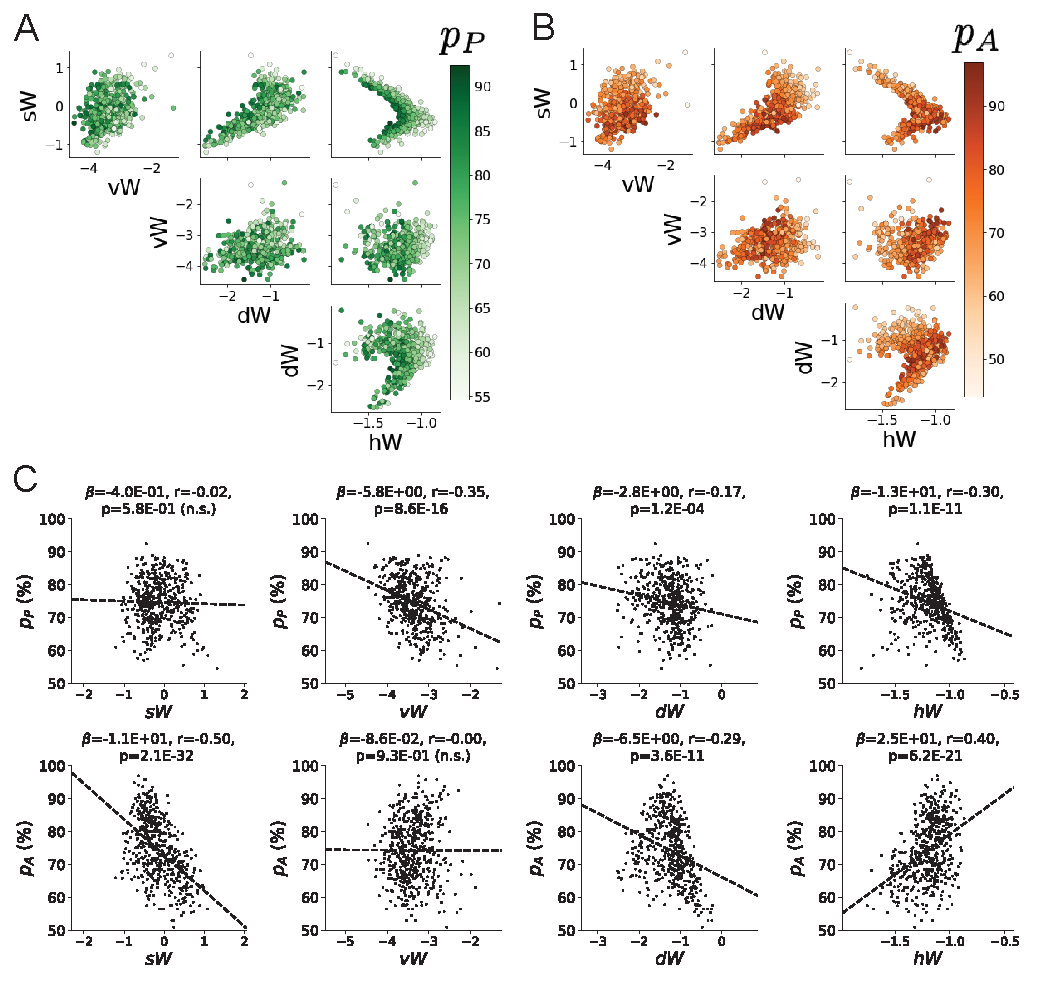
\includegraphics[scale=0.9]{figures/figSC1/figSC1.pdf}
\end{center}
\caption{\small (SC1): \textbf{A}. Same pairplot as Fig. \ref{fig:SC}C colored by Pro task accuracy.  
\textbf{B}. Same as A colored by Anti task accuracy.  
\textbf{C}. Connectivity parameters of EPI distributions versus task accuracies.  $\beta$ is slope coefficient of linear regression, $r$ is correlation, and $p$ is the two-tailed p-value.
}
\label{fig:SC1}
\end{figure}

\begin{figure}
\begin{center}
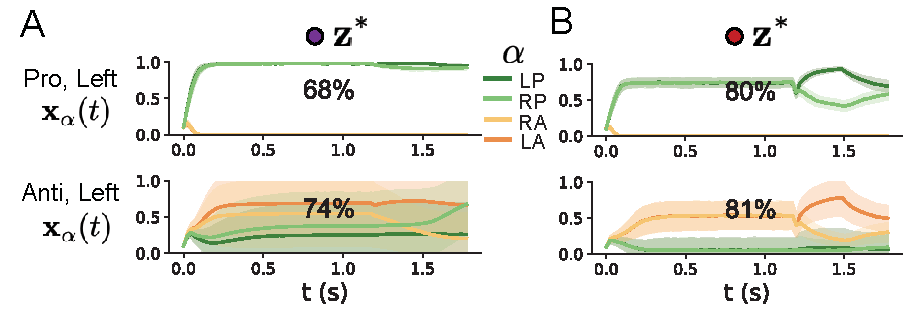
\includegraphics[scale=0.8]{figures/figSC2/figSC2.pdf}
\end{center}
\caption{\small (SC2):  
\textbf{A}. Simulations in network regime $\mathbf{z}_1$ (center) with simulations given connectivity perturbations in the negative direction of the sensitivity vector $\mathbf{v}_1$ (left) and positive direction (right).
\textbf{B}. Same as A for network regime $\mathbf{z}_2$.
}
\label{fig:SC2}
\end{figure}

We order the neural populations of $x$ and $u$ in the following manner
\begin{equation}
\mathbf{x} = \begin{bmatrix} x_{LP} \\ x_{LA} \\ x_{RP} \\ x_{RA} \end{bmatrix} \hspace{2cm} \mathbf{u} = \begin{bmatrix} u_{LP} \\ u_{LA} \\ u_{RP} \\ u_{RA} \end{bmatrix},
\end{equation}

which evolve according to
\begin{equation}
\tau \frac{d\mathbf{u}}{dt} = -\mathbf{u} + W\mathbf{x} + \mathbf{h} + d\mathbf{B}.
\end{equation}
with time constant $\tau = 0.09s$, step size 24ms and Gaussian noise $d\mathbf{B}$ of variance $0.2^2$.  
The weight matrix has 4 parameters $sW$, $vW$, $hW$, and $dW$:
\begin{equation}
W = \begin{bmatrix} sW & vW & hW & dW \\ vW & sW & dW  & hW \\ hW & dW & sW & vW \\ dW  & hW & vW  & sW \end{bmatrix}.
\end{equation}

The circuit receives four different inputs throughout each trial, which has a total length of 1.8s.
\begin{equation}
\mathbf{h} = \mathbf{h}_{\text{constant}}  + \mathbf{h}_{\text{P,bias}} + \mathbf{h}_{\text{rule}} +  \mathbf{h}_{\text{choice-period}} + \mathbf{h}_{\text{light}}.
\end{equation}

There is a constant input to every population,
\begin{equation}\mathbf{h}_{\text{constant}} = I_{\text{constant}} [1, 1, 1, 1]\top,
\end{equation}
 a bias to the Pro populations
\begin{equation}\mathbf{h}_{\text{P,bias}} = I_{\text{P,bias}} [1, 0, 1, 0]\top,
\end{equation}
rule-based input depending on the condition
\begin{equation}\mathbf{h}_{\text{P,rule}}(t) = \begin{cases}
                           I_{\text{P,rule}} [1, 0, 1, 0]^\top,& \text{if } t\leq 1.2s \\
                            0,              & \text{otherwise}
                         \end{cases}
\end{equation}
\begin{equation} \mathbf{h}_{\text{A,rule}}(t) = \begin{cases}
                           I_{\text{A,rule}} [0, 1, 0, 1]^\top,& \text{if } t\leq 1.2s \\
                            0,              & \text{otherwise}
                         \end{cases},
\end{equation}
a choice-period input
\begin{equation} \mathbf{h}_{\text{choice}}(t) = \begin{cases}
                           I_{\text{choice}} [1, 1, 1, 1]^\top,& \text{if } t > 1.2s \\
                            0,              & \text{otherwise}
                         \end{cases},
\end{equation}
and an input to the right or left-side depending on where the light stimulus is delivered    
\begin{equation}  \mathbf{h}_{\text{light}}(t) = \begin{cases}
                           I_{\text{light}} [1, 1, 0, 0]^\top,& \text{if } 1.2s < t < 1.5s \text{ and Left} \\
                           I_{\text{light}} [0, 0, 1, 1]^\top,& \text{if } 1.2s < t < 1.5s \text{ and Right} \\
                            0,              & \text{otherwise}
                         \end{cases}.
\end{equation}
The input parameterization was fixed to $I_{\text{constant}} = 0.75$, $I_{\text{P,bias}} = 0.5 $, $I_{\text{P,rule}} = 0.6$,  $I_{\text{A,rule}} = 0.6$,  $I_{\text{choice}} = 0.25$,  and $I_{\text{light}} = 0.5$.


\begin{figure}
\begin{center}
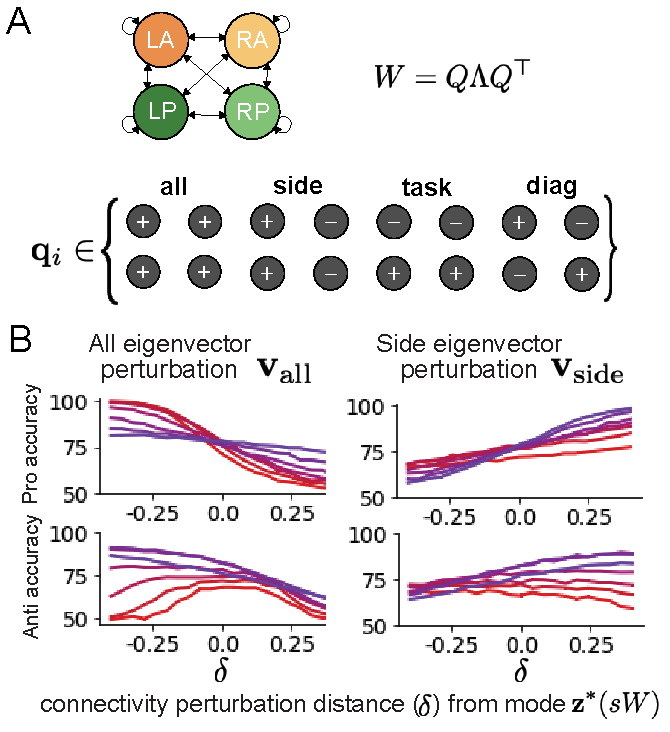
\includegraphics[scale=0.9]{figures/figSC3/figSC3.pdf}
\end{center}
\caption{\small (SC3):  
\textbf{A}. Invariant eigenvectors of connectivity matrix $W$.
\textbf{B}. Eigenvalues of connectivities of EPI distribution versus task accuracies.
}
\label{fig:SC3}
\end{figure}

The accuracies of $p_P$ and $p_A$ are calculated as
\begin{equation}
p_P(\mathbf{x}; \mathbf{z}) = \mathbb{E}_{\mathbf{x} \sim p(\mathbf{x} \mid \mathbf{z})}\left[\Theta[x_{LP}(t=1.8s) - x_{RP}(t=1.8s)]\right]
\end{equation}
and 
\begin{equation}
p_A(\mathbf{x}; \mathbf{z}) = \mathbb{E}_{\mathbf{x} \sim p(\mathbf{x} \mid \mathbf{z})}\left[\Theta[x_{RP}(t=1.8s) - x_{LP}(t=1.8s)]\right]
\end{equation}
given that the stimulus is on the left side, where $\Theta$ is the Heaviside step function, and the accuracy is averaged over 200 independent trials.  The Heaviside step function is approximated as
\begin{equation}
\Theta(\mathbf{x}) = \text{sigmoid}(\beta \mathbf{x}),
\end{equation}
where $\beta = 100$.

\begin{figure}
\begin{center}
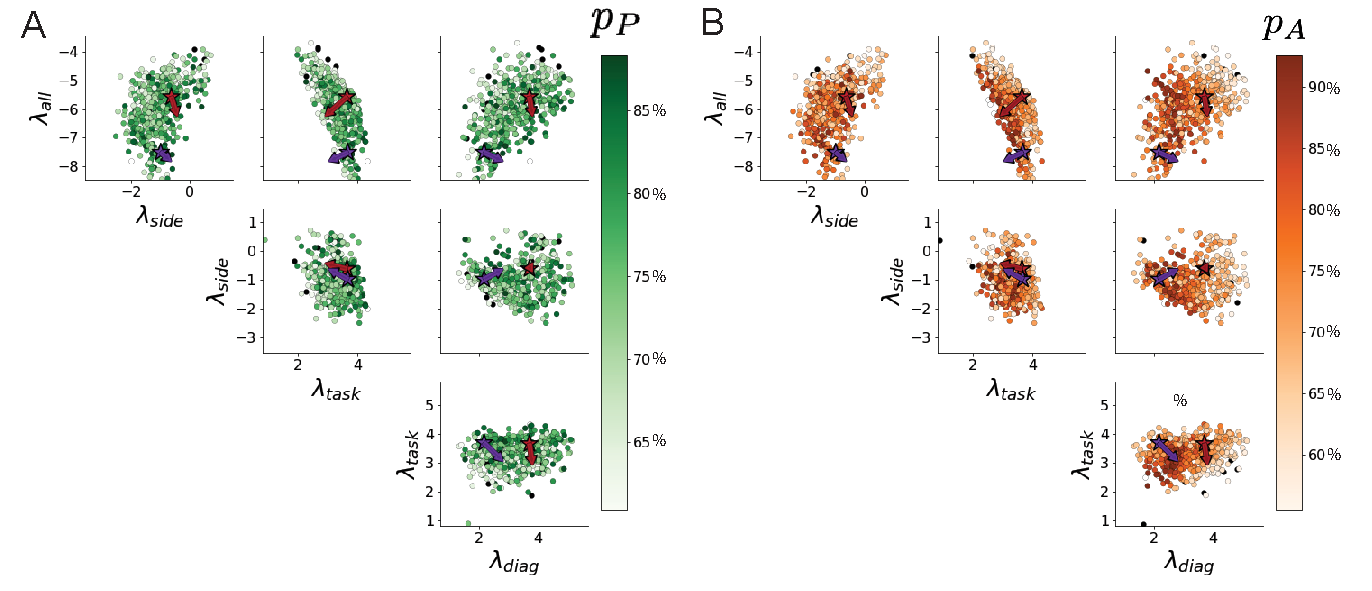
\includegraphics[scale=0.8]{figures/figSC4/figSC4.pdf}
\end{center}
\caption{\small (SC4):  \textbf{A}. Pairplots of eigenvalues of connectivity matrices in EPI distribution colored by Pro task accuracy.  Red and purple stars and arrows correspond to eigenvalues and sensitivity directions $\mathbf{z}_1$, $\mathbf{z}_2$, $\mathbf{v}_1$, and $\mathbf{v}_2$. \textbf{B}. Same colored by Anti task accuracy.
}
\label{fig:SC4}
\end{figure}

\begin{figure}
\begin{center}
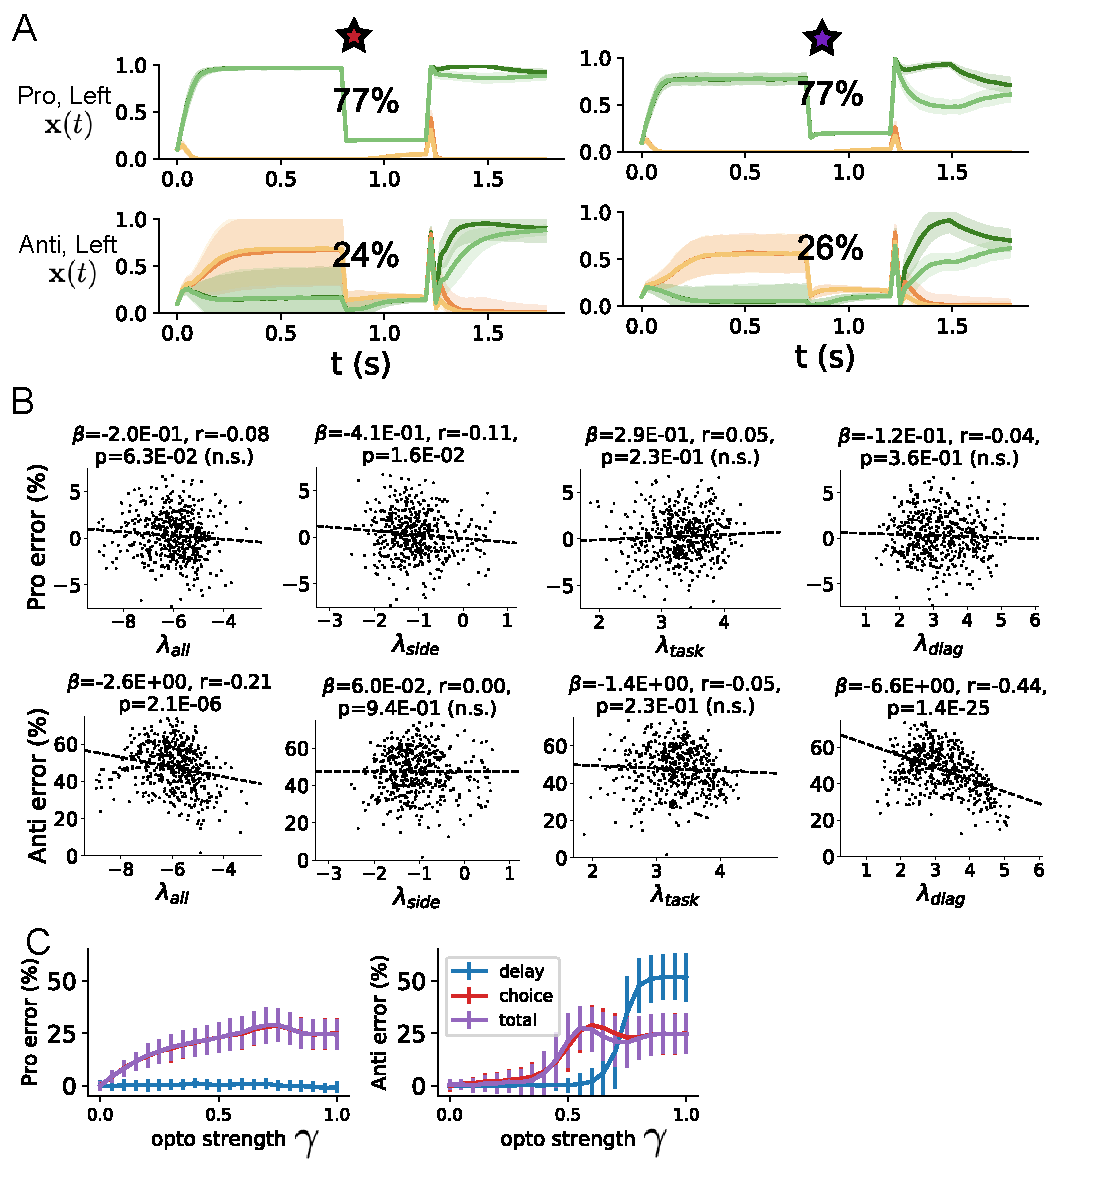
\includegraphics[scale=0.8]{figures/figSC5/figSC5.pdf}
\end{center}
\caption{\small (SC5): 
\textbf{A}. Response of each parameter regime to optogenetic silencing during the delay period.
\textbf{B}. Connectivity eigenvalues versus the task error induced by delay period inactivation.
\textbf{C}. Error induced by delay period inactivation with increasing optogenetic strength.  Means and standard deviations are calculated across the entire EPI posterior.
}
\label{fig:SC5}
\end{figure}

Writing the EPI posterior as a maximum entropy distribution, $T(\mathbf{x}, \mathbf{z})$ is comprised of both these first and second moments of the accuracy in each task (as in Equations \ref{eq:moments} and \ref{eq:mu_opt})
\begin{equation} 
T(\mathbf{x}; \mathbf{z}) = \begin{bmatrix} p(\mathbf{x}; \mathbf{z})_P \\ p(\mathbf{x}; \mathbf{z})_A \\ \left(p(\mathbf{x}; \mathbf{z})_P - 75\% \right)^2 \\ \left(p(\mathbf{x}; \mathbf{z})_A - 75\% \right)^2 \end{bmatrix},
\end{equation}
\begin{equation} 
\bm{\mu}_{\text{opt}} = \begin{bmatrix} 75\% \\ 75\% \\ 7.5\%^2 \\ 7.5\%^2 \end{bmatrix}.
\end{equation}
Throughout optimization, the augmented Lagrangian parameters $\eta$ and $c$, were updated after each epoch of 2,000 iterations(see Section \ref{methods_AL_opt}).  
The optimization converged after six epochs (Fig. \ref{fig:SC5}).


\begin{figure}
\begin{center}
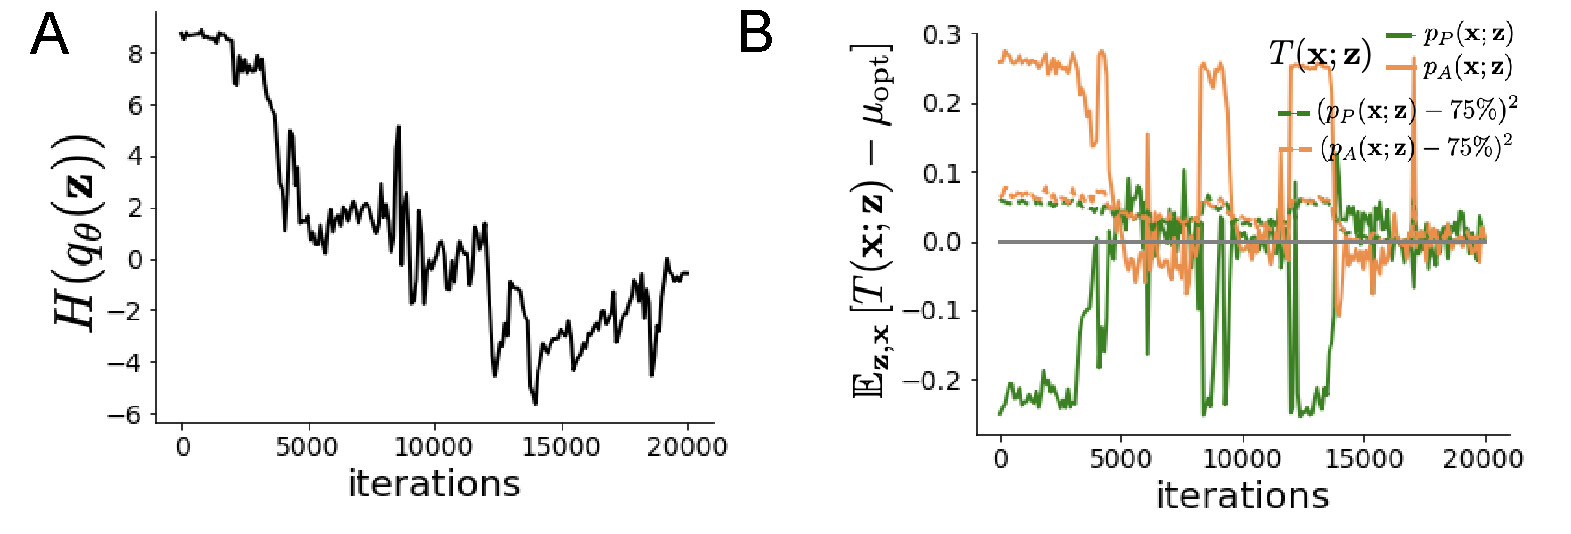
\includegraphics[scale=0.5]{figures/figSC6/figSC6.pdf}
\end{center}
\caption{\small (SC6): 
A. Entropy throughout optimization. 
B. The emergent property statistic means and variances converge to their constraints at 20,000 iterations following the tenth augmented Lagrangian epoch.
}
\label{fig:SC5}
\end{figure}

For EPI in Fig. \ref{fig:SC}C, we used a real NVP architecture with three coupling layers of affine transformations parameterized by two-layer neural networks of 50 units per layer.
The initial distribution was a standard isotropic gaussian $z_0 \sim \mathcal{N}(\mathbf{0}, I)$ mapped to a support of $\mathbf{z}_i \in [-5, 5]$. 
We used an augmented Lagrangian coefficient of $c_0 = 10^{2}$, a batch size $n=100$, and $\beta=2$.
The distribution shown is that of the architecture converging with criteria $N_{\text{test}} = 25$ at greatest entropy across random seeds.

To make sense of this inferred distribution, we identified two modes used to represent the two regimes of connectivity in this posterior:
\begin{equation}
\begin{split}
\mathbf{z}_1 = &\argmax_{\mathbf{z}} \log q_{\bm{\theta}}(\mathbf{z} \mid \mathcal{X}) \\
&\text{s.t. }  hw = -1.25\text{, }  sW > 0
\end{split}
\end{equation}
and 
\begin{equation}
\begin{split}
\mathbf{z}_2 = &\argmax_{\mathbf{z}} \log q_{\bm{\theta}}(\mathbf{z} \mid \mathcal{X}) \\
&\text{s.t. } hw = -1.25\text{, } sW < 0
\end{split}
\end{equation}

To understand the connectivity mechanisms governing task accuracy, we took the eigendecomposition of the symmetric connectivity matrices $W = V\Lambda V^{-1}$, which results in the same basis vectors $\mathbf{v}_i$ for all $W$ parameterized by $\mathbf{z}$ (Fig. \ref{fig:SC3}A). 
These basis vectors have intuitive roles in processing for this task, and are accordingly named the \textit{all} mode - all neurons co-fluctuate, \textit{side} mode - one side dominates the other, \textit{task} mode - the Pro or Anti populations dominate the other, and \textit{diag} mode - Pro- and Anti-populations of opposite hemispheres dominate the opposite pair. 
We found significant trends across the EPI posterior connectivities: the eigenvalues $\lambda_{\text{task}}$ and $\lambda_{\text{diag}}$ were correlated with $p_P$, while $\lambda_{\text{all}}$ was anticorrelated with $p_P$.
$\lambda_{\text{all}}$, $\lambda_{\text{side}}$, and $\lambda_{\text{diag}}$ were all significantly anticorrelated with $p_A$.

Under this decomposition, we can re-visualize the posterior in eigenvalue space (Fig. \ref{fig:SC4}).
Furthermore, we can project the dimensions of sensitivity into eigenvalue space as well, giving us a more intuitive sense of how connectivity affects computation in each regime.
We see that sensitivity dimensions $\mathbf{v}_1$ and $\mathbf{v}_2$, which cause $p_P$ to increase and a regime dependent change in $p_A$, both point in the direction of increasing $\lambda_{\text{side}}$ and decreasing $\lambda_{\text{task}}$.
These eigenvalue changes are evident in the simulations of connectivity perturbations away from the modes (Fig. \ref{fig:SC2}).
As the component of connectivity along $\mathbf{v}_1$ and $\mathbf{v}_2$ becomes stronger (left-to-right), there is less separation between Pro an Anti populations (lower $\lambda_{\text{task}}$) and greater separation between Left and Right populations following stimulus presentation (greater $\lambda_{\text{side}}$).
A key differentiating factor is that $\mathbf{v}_1$ substantially increases $\lambda_{\text{diag}}$, while $\mathbf{v}_2$ does not.

During optogenetic silencing simulations, activations $x_\alpha(t)$ were set to a fraction of their values ($1 - \gamma$), where $\gamma$ is the optogenetic perturbation strength.
We found that $\lambda_{\text{all}}$ and $\lambda_{\text{diag}}$ were significantly anticorrelated with Anti error during delay period inactivation.
Delay period inactivation was from $0.8 < t < 1.2$, choice period inactivation was for $t > 1.2$ and total inactivation was for the entire trial.

\subsubsection{Rank-2 RNN}\label{methods_RNN}
Traditional approaches to likelihood-free inference -- approximate Bayesian computation (ABC) methods -- randomly sample parameters $\mathbf{z}$ until a suitable set is obtained.
State-of-the-art ABC methods leverage sequential Monte Carlo (SMC) sampling techniques to obtain parameter sets more efficiently.
To obtain more parameter samples, SMC-ABC must be run from scratch again.
ABC methods do not confer log probabilities of samples.
 Like EPI, sequential neural posterior estimation (SNPE) uses deep learning to produce flexible posterior approximations.
Like traditional Bayesian inference methods, SNPE conditions directly on the statistics of data.
This differs from EPI, where posteriors are conditioned on emergent properties (moment constraints on the posterior predictive distribution).
Peculiarities of SNPE (density estimation approach, two deep networks) make scaling in $\mathbf{z}$ prohibitive.

SMC-ABC has many hyperparameters, of which pyABC selects automatically by running some initial diagnostics upon initialization.
In concurrence with the literature, SMC-ABC fails to converge around 25-30 dimensions, since it's proposal samples never get close enough to the target statistics.
We searched over many SNPE hyperparameter choices: $n_{\text{train}} \in [2,000, 10,000, 100,000]$ is the number of simulations run per training epoch, and $n_{\text{mades}} \in [2, 3]$ is the number of masked autoregressive density estimators in the deep parameter distribution architecture.  
The greater $n_{\text{train}}$, the longer each epoch will take, but the more likely SNPE may converge during that epoch.
Greater $n_{\text{mades}}$ increases the flexibility of the deep parameter distribution of SNPE, but slows optimization.
For the timing plot, we show the fastest among all of these choices, and for the convergence plot, we show the best convergence among all of these choices.
During optimization, we used $n_{\text{atom}}$=100 atomic proposals as is recommended.

%\subsubsection{Rank-1 RNN}\label{methods_LRRNN}
%Extensive research on random fully-connected recurrent neural networks has resulted in foundational theories of their activity \cite{sompolinsky1988chaos, brunel2000dynamics}.
%Furthermore, independent research on training these models to perform computations suggests that learning occurs through low-rank perturbations to the connectivity (e.g. \cite{jaeger2004harnessing, sussillo2009generating}).
%Recent theoretical work extends theory for random neural networks \cite{sompolinsky1988chaos} to those with added low-rank structure \cite{mastrogiuseppe2018linking}.
%In Section \ref{results_RNN}, we used this theory to enable EPI on RNN parameters conditioned on the emergent property of task execution.
%
%Such RNNs have the following dynamics: 
%\begin{equation}
%\frac{dx}{dt} = -x + W \phi(x) + h,
%\end{equation}
%where $x$ is network activity, $W$ is the connectivity weight matrix, $\phi(\cdot) = \tanh(\cdot)$ is the input-output function, and $h$ is the input to the system.
%In a rank-1 RNN (which was sufficiently complex for the Gaussian posterior conditioning task), $W$ is the sum of a random component with strength $g$ and a structured component determined by the outer product of vectors $m$ and $n$:
%\begin{equation}
%W = g\chi + \frac{1}{N}mn^\top,
%\end{equation}
%where  $\chi_{ij} \sim \mathcal{N}(0, \frac{1}{N})$, and the entries of $m$ and $n$ are distributed as $m_i \sim \mathcal{N}(M_m, 1)$ and $n_i \sim \mathcal{N}(M_n, 1)$. 
%For EPI, we consider $z = [g, M_m, M_n]$, which are the parameters governing the connectivity properties of the RNN.
%
%From such a parameterization $z$, the theory of Mastrogiuseppe et al. produces solutions for variables describing the low dimensional response properties of the RNN.
%These ``dynamic mean field" (DMF) variables (e.g. the activity along a vector $\kappa_v$, the total variance $\Delta_0$, structured variance $\Delta_\infty$, and the chaotic variance $\Delta_T$) are derived to be functions of one another and connectivity parameters $z$.
%The collection of these derived functions results in a system of equations, whose solution must be obtained through a nonlinear system of equations solver.
%The iterative steps of this system of equations solver are differentiable, so we take gradients through this solve process.
%The DMF variables provide task-relevant information about the RNN's response to task inputs.
%
%In the Gaussian posterior conditioning example, $\kappa_r$ and $\Delta_T$ are DMF variables used as task-relevant emergent property statistics $\mu_{\text{post}}$ and $\sigma^2_{\text{post}}$.
%Specifically, we solve for the DMF variables $\kappa_r$, $\kappa_n$, $\Delta_0$ and $\Delta_\infty$, where the readout is nominally chosen to point in the unit orthant $r = [1, ..., 1]^\top$.  
%The consistency equations for these variables in the presence of a constant input $h = y r - (n - M_n)$ can be derived following \cite{mastrogiuseppe2018linking}:
%{\small
%\begin{equation}
%\begin{split}
%\kappa_r = G_1(\kappa_r, \kappa_n, \Delta_0, \Delta_\infty) = M_m \kappa_n + y \\
%\kappa_n = G_2(\kappa_r, \kappa_n, \Delta_0, \Delta_\infty) = M_n \langle \left[ \phi_i \right] \rangle + \langle \left[ \phi_i' \right] \rangle \\
%\frac{\Delta_0^2-\Delta_\infty^2}{2} = G_3(\kappa_r, \kappa_n, \Delta_0, \Delta_\infty) = g^2 \left( \int \mathcal{D}z \Phi^2(\kappa_r + \sqrt{\Delta_0}z) - \int \mathcal{D}z \int \mathcal{D}x \Phi(\kappa_r + \sqrt{\Delta_0 - \Delta_\infty}x + \sqrt{\Delta_\infty}z)  \right) \\
%+ (\kappa_n^2  + 1)(\Delta_0-\Delta_\infty) \\
%\Delta_\infty = G_4(\kappa_r, \kappa_n, \Delta_0, \Delta_\infty)  = g^2 \int \mathcal{D}z \left[ \int \mathcal{D}x \phi(\kappa_r + \sqrt{\Delta_0 - \Delta_\infty}x + \sqrt{\Delta_\infty}z \right]^2 + \kappa_n^2 + 1
%\end{split} 
%\end{equation}
%}
%where here $z$ is a gaussian integration variable. 
%We can solve these equations by simulating the following Langevin dynamical system to a steady state:
%
%\begin{equation}
%\begin{split}
%l(t) = \frac{\Delta_0(t)^2-\Delta_\infty(t)^2}{2} \\
%\Delta_0(t) = \sqrt{2l(t) + \Delta_\infty(t)^2} \\
%\frac{d \kappa_r(t)}{dt}  = -\kappa_r(t) + G_1(\kappa_r(t), \kappa_n(t), \Delta_0(t), \Delta_\infty(t)) \\
%\frac{d \kappa_n(t)}{dt} = -\kappa_n + G_2(\kappa_r(t), \kappa_n(t), \Delta_0(t), \Delta_\infty(t)) \\
%\frac{d l(t)}{dt}  = -l(t) + G_3(\kappa_r(t), \kappa_n(t), \Delta_0(t), \Delta_\infty(t)) \\
%\frac{d \Delta_\infty(t)}{dt}  = -\Delta_\infty(t) + G_4(\kappa_r(t), \kappa_n(t), \Delta_0(t), \Delta_\infty(t))
%\end{split}.
%\end{equation}
%Then, the chaotic variance, which is necessary for the Gaussian posterior conditioning example, is simply calculated via $\Delta_T = \Delta_0 - \Delta_\infty$.
%
%We ran EPI using a real NVP architecture of two masks and two layers per mask with 10 units mapped to a support of $z = [g, M_m, M_n] \in [0,5] \times [-5,5] \times[-5,5]$ with no batch normalization. 
%We used an augmented Lagrangian coefficient of $c_0 = 1$, a batch size $n=300$, set $\nu = 0.15$, and initialized $q_{\bm{\theta}}(z)$ to produce an isotropic Gaussian with mean $\mu_{\text{init}} = [2.5, 0, 0]$ with standard deviation $\sigma_{\text{init}} = 2.0$.
%The EPI distribution shown in Fig. \ref{fig:RNN} is the converged distributions with maximum entropy across five random seeds.
%
%To examine the effect of product $M_m M_n$ on the posterior mean, $\mu_{\text{post}}$ we took perturbations in $M_m M_n$ away from two representative parameters  $z_1$ and $z_2$ in 21 equally space increments from -1 to 1.  
%For each perturbation, we sampled 10 2,000-neuron RNNs and measure the calculated posterior means.  
%In Fig. \ref{fig:RNN}D, we plot the product of $M_m M_n$ in the perturbation versus the average posterior mean across 10 network realizations with standard error bars.  
%The correlation between perturbation product $M_m M_n$ and $\mu_{\text{post}}$ was measured over all simulations.  
%For perturbations away from $z_1$ the correlation was 0.995 with $p<10^{-4}$, and for perturbations away from $z_2$ the correlation was 0.983 with $p<10^{-4}$.
%
%In addition to the Gaussian posterior conditioning example in Section \ref{results_RNN}, we modeled two tasks from Mastrogiuseppe et al.: noisy detection and context-dependent discrimination.  
%We used the same theoretical equations and task setups described in their study.
\end{document}

